\chapter{Data Analysis I: Calibration and Corrections}

\section{S$\pi$RITROOT Software}
\label{sec:software}

The S$\pi$RITROOT software is modular code based on the FAIRROOT package written in C++ \cite{fairroot}. The code is separated into modules which can be turned on or off depending on the users needs. The base classes and frame work is provided by the FAIRROOT package, while the specifics of each detector need to be added into the base classes. In the following an outline of the main tasks in the S$\pi$RITROOT software will be briefly discussed with the details of each task discussed later. The discussion of the software is really a practical, base understanding, appropriate for this thesis. For more details about the tracking algorithm the reader is refered to \cite{spiritroot_paper}, and to actual software which is published on GitHub \cite{spiritroot_git}. 

The main tasks which make up the reconstruction algorithm are:

\begin{itemize}
  \item Decoder task
  \item Pulse Shape Algorithm (PSA Task)
  \item Helix Track Finding Algorithm
  \item Track Fitting and momentum reconstruction(GENFIT package)
  \item Vertex Reconstruction (RAVE package).
\end{itemize}


\subsection{Decoder task}
The decoder task reads in the raw data output from the GET electronics and separates the data from the headers using the GETDecoder \cite{getdecoder}. A map is stored mapping each channel in the CoBo board onto the physical pad plane, the information is stored in a pad container called the STPad class. This container stores the row, layer, and the raw ADC time bucket spectrum. All of the pads combined form the event container, STRawEvent class, which represents the raw event information. 

Three basic calibrations are performed at the raw data level within this task. The gain calibration calibrates the electronics will be described in Section\ref{sec:elecCalib} and the anode gain calibration is discussed in Section~\ref{sec:anodeCalib}. The gating grid noise subtraction and time bucket cut which is described in Section~\ref{sec:ggnoisesub}.
%gain calibration 
%ggnoise subtraction
%GG time bucket cut


\subsection{Pulse Shape Algorithm (PSA) Task}
\label{sec:psa}
%Yoffset match the TPC-Vertex_y with BDC_Y
%YPedestalOffset what is it for?
%cobo gain matching
An algorithm loops over the raw time bucket spectrum to find all the unique pules in each pad. It is very likely that there are several pulses in a pad coming from multiple tracks passing under the same pad which are separated only in arrival time. Figure~\ref{fig:psaTask} shows the PSA task working on one particular pad in experimental data. The shaded histogram in every sub-figure represents the ADC raw spectrum of the pad. In Fig.~\ref{fig:psa0} we see the PSA has identified the first pulse and fitted it with the standard pulse, the result of the fit is shown by the red line. The fitted red line is then subtracted from the ADC spectrum, which is shown in the shaded histogram in Fig.~\ref{fig:psa1}. Here, the second pulse is found and fitted again with the same procedure, the red line will be subtracted from the raw ADC spectrum. The black line represents the sum of all the fitted pules in each step. This continues until all pules are found or until the PSA reaches the last bin in the spectrum. Figure~\ref{fig:psa4} shows the final result where 4 fitted pulses were found. The agreement between the total summed line and the raw ADC spectrum exemplifies how successful the PSA is in this particular set of data. 

%Mention about the minimum distance between hits? 



The fit of each individual pulse contains the height of the pulse and the timing information of the start of the pulse, defined to be the location in time of 10\% of the rising edge. The height of the pulse, which is related to the charge induced on the pad, $Q$, and the timing information $t_o$, is saved into a new container representing a ``hit", called the STHit class. After the PSA processes each pad in the raw event, an entire hit cloud of the event is produced. The x and z-coordinates come from the center of the pad which is already stored in the map of STPad. Since the STHit class inherits from the STPad class this information is also carried over. The y-coordinate is calculated using the known drift velocity $v$ and time of the signal $t_o$ as $y = v\cdot t_0$, $t_0$. The hit class forms the fundamental structure from which all tracking is performed since it contains the x,y,z spacial coordinates, and charge information $Q$.


\begin{figure}[!htb]
     \centering
     \begin{subfigure}[b]{0.24\textwidth}
         \centering
         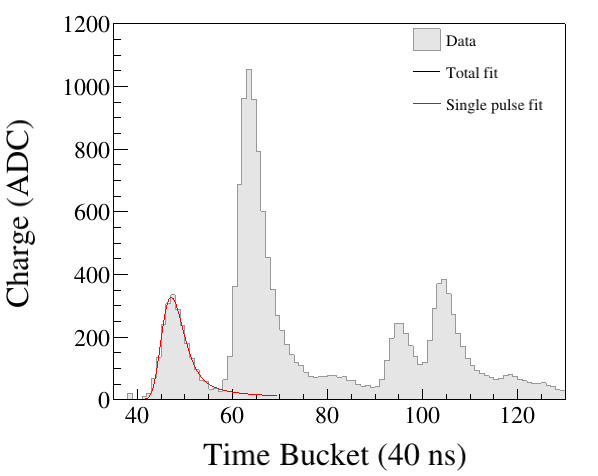
\includegraphics[width=\textwidth]{psa0.png}
         \caption{$\mathrm{1^{st}}$ step of the PSA}
         \label{fig:psa0}
     \end{subfigure}
     \hfill
     \centering
     \begin{subfigure}[b]{0.24\textwidth}
         \centering
         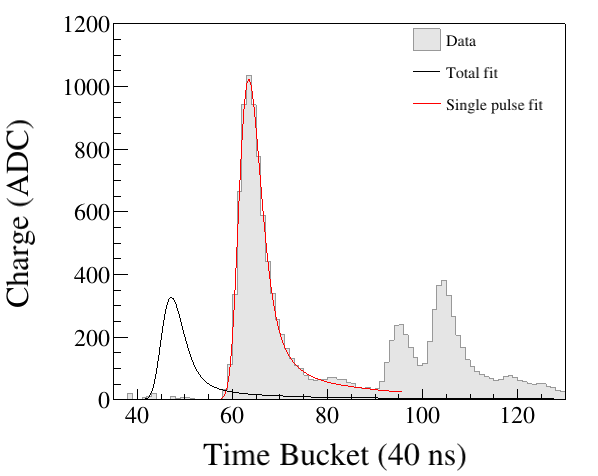
\includegraphics[width=\textwidth]{psa1.png}
         \caption{$\mathrm{2^{nd}}$ iteration}
         \label{fig:psa1}
     \end{subfigure}
     \hfill
      \centering
     \begin{subfigure}[b]{0.24\textwidth}
         \centering
         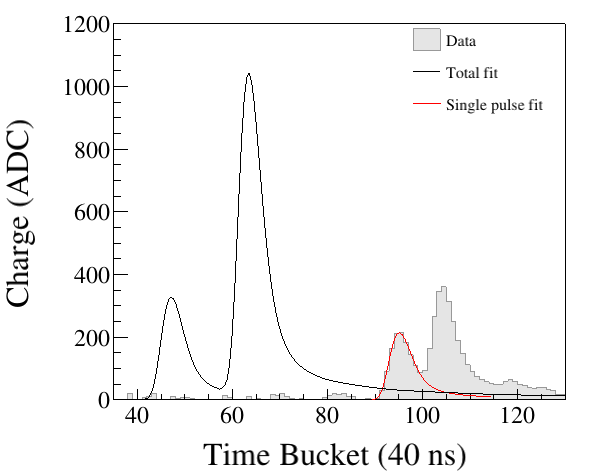
\includegraphics[width=\textwidth]{psa2.png}
         \caption{$\mathrm{3^{rd}}$ iteration}
         \label{fig:psa2}
     \end{subfigure}
     \hfill
      \centering
     \begin{subfigure}[b]{0.24\textwidth}
         \centering
         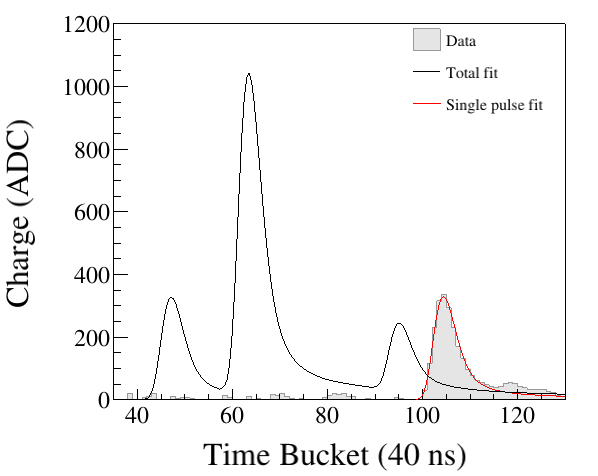
\includegraphics[width=\textwidth]{psa3.png}
         \caption{$\mathrm{4^{th}}$ iteration}
         \label{fig:psa3}
     \end{subfigure}
     \hfill
     \centering
     \begin{subfigure}[b]{.5\textwidth}
         \centering
         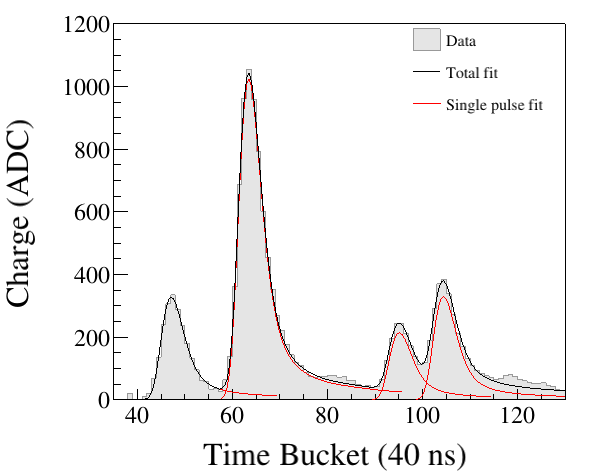
\includegraphics[width=\textwidth]{psa4.png}
         \caption{Final output of the PSA}
         \label{fig:psa4}
     \end{subfigure}
     \hfill
    
\caption{Example of the pulse shape algorithm through each step of in processing a given pad. }
\label{fig:psaTask}
\end{figure}


\subsection{Helix Tracking}
%Cluster cut
%ellipsoid cut
\label{sec:helixtrack}

 The function of the  helix track finding algorithm is to sort hit cloud into unique sets of hits representing tracks. This is performed by a Riemann track finding algorithm where the Cartesian space is mapped onto a Riemann sphere. This is a particular transformation in which unique helices in the Cartesian space form great circles on the Riemann sphere. This is particularly useful since hits which correspond to a track form a helices the Cartesian space of the TPC coordinates. It is difficult to search for tracks in the hit cloud by fitting a general helix to different combinations of hits. It is much easier to search for collection of hits by fitting a plane to the great circles which are formed on the Riemann sphere. From here the set of hits which form a unique track are stored into a new helix track container called the STHelixTrack class. 
 

\paragraph{Definition of clustering}
The hits within a helix track are dense and the position resolution of an individual hit is not very precise. As mentioned in Section~\ref{sec:prf}, the TPC can achieve sub-millimeter position resolution by utilizing the PRF. In the helix track finding task, the hits are further reduced into more precise clusters. A brief description of the method of clustering is illustrated in Figure \ref{fig:topview}. As will be seen, it is sufficient to simply cluster hits along one direction, either along the x or z-direction, which ever is most perpendicular to the local track region. For example, the three clusters at the bottom of Figure \ref{fig:topview} are clustered along the x-axis, and the upper three are along the z-axis. The bold pads highlight the hits belonging to an example cluster from each set. Since we decide to cluster only in one direction, there is a natural inflection point in a track at which the direction of clustering must switch. This depends on the crossing angle of the track $\theta$, which is defined as the angle between the tangent of the track  at that cluster and the x-axis. In this definition $\theta = \ang{90}$ when the track is going along the z-axis and $\theta = \ang{0}$ for a track going along the x-axis.  The clustering direction in the case $\ang{45} < \theta \leq \ang{90} $ is along the x-direction. For $\ang{0} < \theta \leq \ang{45}$ we cluster along the z-axis. 

 

\begin{figure}[!htb]
\centering
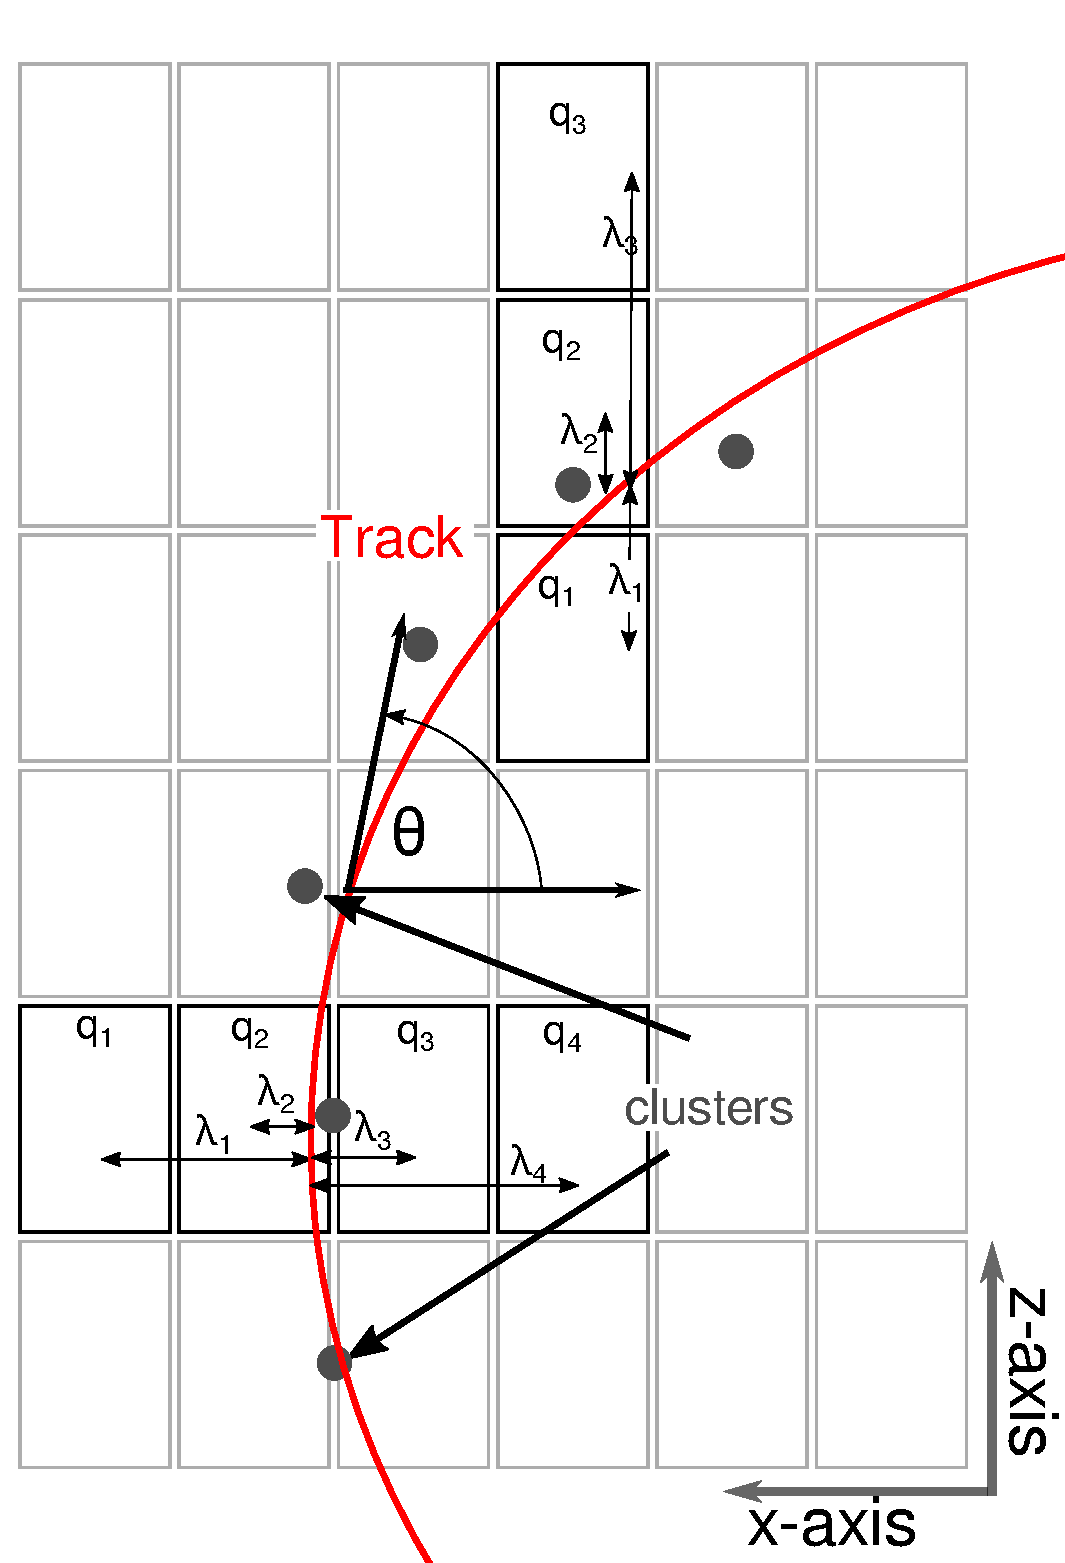
\includegraphics[scale=.5]{top_view_helix_ext.pdf}
\caption{Cartoon graphic of a top down view of a fit to a track passing through several pads. The bolded pads and the charges $q_i$ represent the hits belonging to that pad and the clusters of the track representing the average position of the track. The three clusters at the bottom are clustered in the x-direction and for the upper three clustered in the z-direction. The estimate of the position of the avalanche is given by the track fit and the position from the center to each pad to the $\bar{x}$ position is given as $\lambda_i$.}
\label{fig:topview}
\end{figure}

 The position along the clustering direction, $\overline{X}$, is calculated as the charge-weighted average, $\overline{X} = \sum_i q_ix_i$, where $q_i$ and $x_i$ are the charge and position of the i-th hit in the cluster. The other direction is set to the center of the pad. For example, if we are clustering hits along the x-axis, the z-position is set to the center of the pad in the z-direction and vice versa. Switching the clustering direction gives better position resolution than if we clustered only along one direction. You can imagine if we calculated the clusters only along the x-axis for tracks with $\theta \approx 0^{\circ}$ the x-position is not well defined. The cluster position and charge is stored into a new container represented the cluster called the STHitCluster class. All the clusters which belong to a particular helix track is also stored in the corresponding STHelixTrack class. 

\subsection{Correction Task}
%extend dynamic range
%PRF cut
%space charge correciton
In this task the hit distribution, within a given cluster, is checked against the measured PRF discussed in Section~\ref{sec:prf}. Figure~\ref{fig:prfpimData} shows black lines around the measured PRF in the data, which form gates defining the acceptable PRF region. If less than 50\% of the hits within a cluster lie within this gate, the cluster is thrown out from the track. A majority of the clusters contains either 2 or 3 hits in total; in the case of 2 total hits, at least one of them needs to lie in the gate, in the case of 3 total hits, at least 2 hits need to lie within the gate. Clusters which do not follow this PRF gate usually have been corrupted. Typically charges from other nearby tracks is the typical way clusters become corrupt.  

%CONSIDER SHOWING SOME PROOF OF IT IN ACTION 

This correction task also handles several other important corrections. The first is a novel algorithm which extends the dynamic range of the electronics and is discussed in detail in Section~\ref{sec:extendDynamicRange}. The other correction task that is handled here is the space charge correction which will be discussed in more detail in Section~\ref{sec:spacecharge}. 

\subsection{Momentum and track reconstruction (GENFIT)}
After all of the corrections are applied to the clusters, the cluster's position and charge values are passed to a software package which reconstructs the momentum of the track, called GENFIT \cite{genfit}. The details of Kalman fitting algorithm used in the GENFIT reconstruction are left for the reader here \cite{genfit}. GENFIT returns a momentum and charge value for the track which is stored into a new track container called the STRecoTrack class. 

The task is repeated a second time, storing a second copy of the track class but this time with the BDC vertex point added as a constraining cluster. The momentum resolution is greatly improved by adding the vertex as a constraining point; since the BDC detectors, described in Section~\ref{sec:bdc}, give such an accurate vertex location. The energy loss of the track is calculated by the truncated mean method described in Eq.~\ref{eq:truncmean}. This is the final part of the analysis which pertains to tracks, and the PID can be constructed using the energy loss, momentum, and charge information. 

\subsection{Vertex tracking (RAVE)}
\label{sec:vertex}
After all tracks are reconstructed by GENFIT, the tracks are then passed to the RAVE software package which reconstructs the event vertex from a collection of tracks \cite{rave}. Only tracks which are THIS CONDITION are used in making the event vertex. The vertex location along the beam axis determines whether or not the beam collided with the target. 


\section{Calibrations and Corrections}
In the following subsections we will discuss in detail the calibrations and corrections happening within the software framework that was outlined above.  

\subsection{Gating grid noise subtraction}
\label{sec:ggnoisesub}
The opening of the gating grid is essentially shorting adjacent wires in the grid together, allowing them to reach equilibrium as fast as possible. Since the impedance of both sides was not entirely matched properly this caused an imbalance of charge which bounce back and forth in the grid in an under-dampened manner. This oscillating charged induced  residual induced signals early in the time bucket spectrum creating extra source of noise in the data. Figure~\ref{fig:ggNoiseSub} shows in the upper panel the gating grid noise ADC time bucket spectrum for 2000 events in a given pad. The gating grid noise is stable for a given pad and the mean value --shown as the red line-- can be calculated after averaging over several thousands events. The raw gating grid noise lasts for 100 Tbs extending into the real data with a exponentially decreasing ampli 

 %The ground grid shielded some of the noise, but the path to ground was on two ends and was not sufficiency for this frequency.
 
\begin{figure}[!htb]
\centering
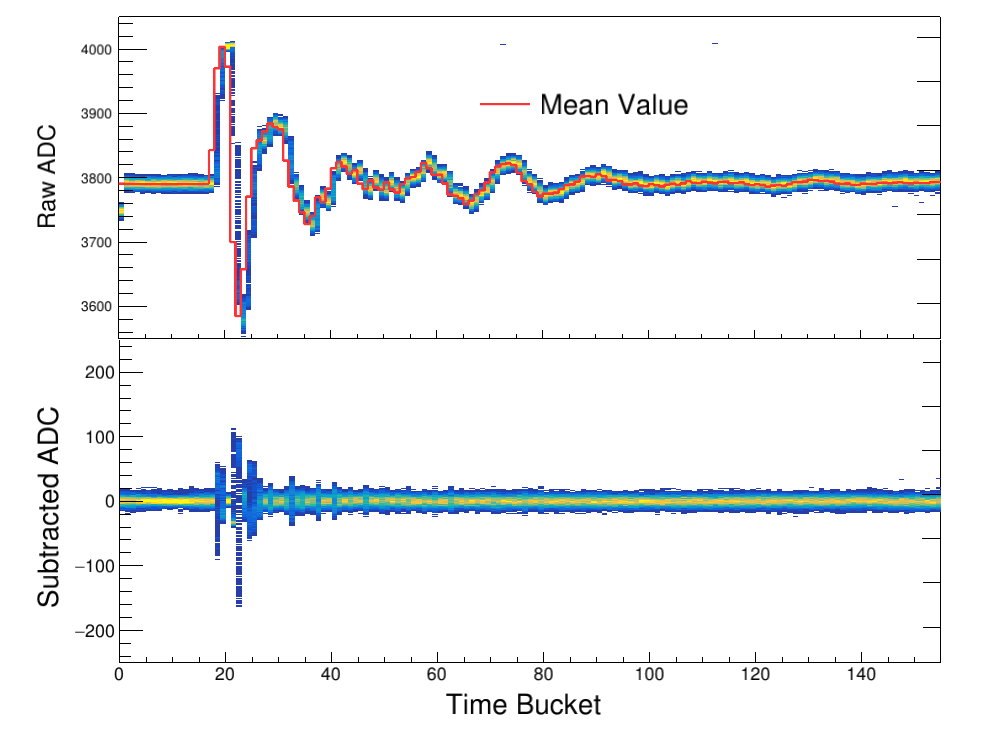
\includegraphics[width=\textwidth]{ggNoise.png}
\caption{Gating grid noise profile and subtraction for a particular pad.}
\label{fig:ggNoiseSub}
\end{figure}

The gating grid noise profile is measured by recording experimental data, only turning off the anode wires. By doing so there are no signals originating from tracks in the TPC and there is only the gating grid noise, since the grid is still being triggered.  The mean value of each pad is calculated from several thousand events of the gating grid noise profile. Once the mean value response in each pad is calculated, we can subtract the mean profile from the real data and remove the noise of the gating grid.

The bottom panel of Fig.~\ref{fig:ggNoiseSub} shows the gating grid noise self correcting itself; a best case scenario. We can see the pedestal, which is around 3800 ADC in the upper pannel,  is automatically taken into account when subtracting the mean profile, and the subtracted ADC spectra is centered around 0. The residual gating grid noise that was not canceled by the subtraction remains, but is significantly reduced to a much smaller time bucket region. Most of the residual noise happens in regions where the derivative of the gating grid noise is large. In these areas the ADC value is dependent upon small jitters in the timing of the signal and as a result varies wildly. The residual noise in the subtracted spectra is removed by cutting away all the bins below 30 tb. 

In the experiment the gating grid itself was quite stable in the  ${}^{132}$Sn and ${}^{124}$Sn systems and was not very stable in the ${}^{108}$Sn and ${}^{112}$Sn beams, where the gating grid broke several times. The gating grid noise was monitored and we regularly took gating grid noise profiles, especially after a gating grid board was replaced. 


%The average noise profile was constructed by averaging all the events in the gating grid runs, pad-by-pad; each pad had a slightly different noise profile since the impedance to each pad was slightly different. It is worth noting that the small electronics noise would be effectively canceled out by averaging over thousands of events. During the first stages of the software, the gating grid noise profile closest to that run would be subtracted from the raw data canceling the gating grid noise in that run. 

\subsection{Cocktail calibration}
\label{sec:cocktail}

\begin{table*}\centering
\ra{1.3}
\begin{tabular}{@{}rrrrrrr@{}}\toprule
& \multicolumn{3}{c}{$100 MeV Target$}\\
\cmidrule{2-4}
Particle &\phantom{abc} & Measured & Corrected & \% Difference & \% Difference\\
\midrule
p   & 882.8 & 929.5 & 877.3   &  3.7  & -1.0  \\
d   & 817.1 & 831.15 & 797.94 &  1.7  & -2.3\\
\bottomrule
\end{tabular}
\caption{Summary of expected cocktail for the calibration run taken with the Al target. }
\label{tb:cocktail100tar}
\end{table*}

\begin{table*}\centering
\ra{1.3}
\begin{tabular}{@{}rrrrrrr@{}}\toprule
& \multicolumn{3}{c}{$100 MeV$}\\
\cmidrule{2-4}
Particle & Expected & Measured & Corrected & \% Difference & \% Difference\\
\midrule
p   & 882.8 & 903.5 & 889.0 &  2.0   & -1.6  \\
d   & 817.1 & 898.5 & 874.5 &  2.1   & -2.7\\
\bottomrule
\end{tabular}
\caption{Summary of expected cocktail from the lower beam energy.}
\label{tb:cocktail100}
\end{table*}

\begin{table*}\centering
\ra{1.3}
\begin{tabular}{@{}rrrrrrr@{}}\toprule
& \multicolumn{3}{c}{$300 MeV$}\\
\cmidrule{2-4}
Particle & Expected & Measured & Corrected & \% Difference Raw & \% Difference Corrected\\
\midrule
d   & 1621 & 1704 & 1612   &  5.1 & -0.6  \\
t   & 1612 & 1691 & 1596   &  4.9  & -1.0\\
${}^{4}$He   & 1613 & 1698 &  5.3 & 1595  & -1.1\\

\bottomrule
\end{tabular}
\caption{Summary of expected cocktail from the higher beam energy.}
\label{tb:cocktail300}
\end{table*}

A cocktail of several light charged particles was produced (p,d,t,${}^{3}$He,${}^{4}$He), and measured in the TPC to provide a momentum calibration of the TPC. The magnetic and slit settings of the dipoles in the BigRIPS spectrometer was set so that the momentum resolution of the beam was $\delta p/p$ < 1\%. Two magnetic rigidity settings were studied, with an empty target. A thick Aluminum target was also inserted to provide a slightly lower energy point for part of the lower rigidity setting, effectively creating three energy calibration points over several particle species. In some cases the certain particles were not able to propagate or were strongly attenuated. 

Since the cocktail beam was a mono-energetic source of particles and the actual momentum resolution was less than 1\%, the observed momentum resolution can be interpreted as the intrinsic TPC momentum resolution. The momentum resolution in general depends on several factors such as the particle's angle, momentum, charge, track multiplicity, etc. This calibration beam represents and ideal situation where the track was parallel to the pad plane and only one particle was measured at one time. The average momentum resolution was measured to be $dp/p = 2\%$ over the full range of particle species for all settings. 

The energy loss resolution can also be directly measured since each energy setting represents a monochromatic source of each particle species, which have a well defined energy loss distribution. The energy loss resolution was measured to be 5\% for all particles over the energy setting measured and is summarized in Table~\ref{tb:momresolution}.

Since the magnetic dipole setting of the BigRIPS spectrometer is well defined, we can calculate the expected momenta of each particle species measured. The enegy losses through various materials in the beam line were propagated using LISE++ software \cite{lise++}. The measured momenta of the calibration beam differed significantly from the expected values -- up to 5\% in the high momentum calibration -- as seen in Tables~\cref{tb:cocktail100tar,tb:cocktail100,tb:cocktail300}. This effect is attributed to inhomogenatities in the magnetic field which introduces electron drift velocities in the direction of $\vec{E}\times\vec{B}$ direction as seen from Eq.\ref{eq:elecdrift}. The $\vec{E}\times\vec{B}$ drift velocity causes the electron trajectories to shift toward the +x-axis in the TPC coordinates causing particles of positive charge (going in the -x-axis) to have a higher measured momenta than in reality.  The details of the correcting for the $\vec{E}\times\vec{B}$ effect will be discussed later in Section~\ref{sec:spacecharge} in a  general way which also includes the correction for the positive space charge. The same correction technique was applied here where the cocktail beam is the special case of zero space charge, only having $\vec{E}\times\vec{B}$ components.

The values under the corrected column in Tables~\cref{tb:cocktail100tar,tb:cocktail100,tb:cocktail300}, represent the corrected data. A significant improvement is seen in the high momentum setting going from around ~5\% disagreement to within ~1\% agreement in the corrected data. For the lower momentum settings (Tables~\cref{tb:cocktail100tar,tb:cocktail100}), protons see a slight improvement of about ~1\% where as the deuterons are over corrected in both settings. The level of agreement of the all corrected values is still well within the estimated momentum resolution of the TPC. 

\begin{table*}\centering
\ra{1.3}
\begin{tabular}{@{}cc@{}}\toprule
Momentum Resolution \% & <dE/dx> Resolution \% \\
\midrule
1.6  & 4.6\\
\bottomrule
\end{tabular}
\caption{Summary of the estimated momentum and energy loss resolutions.}
\label{tb:momresolution}
\end{table*}

%Apendix of the beam line elements
%apendix of the settings of the bigrips elments
%Picture of cocktail before and after ExB effect
%Table of LISE++ expected cocktail energies ridigity setting of dipole magnets (reference big rips line)


\subsection{Electronics calibration}
\label{sec:elecCalib}

\begin{figure}[!htb]
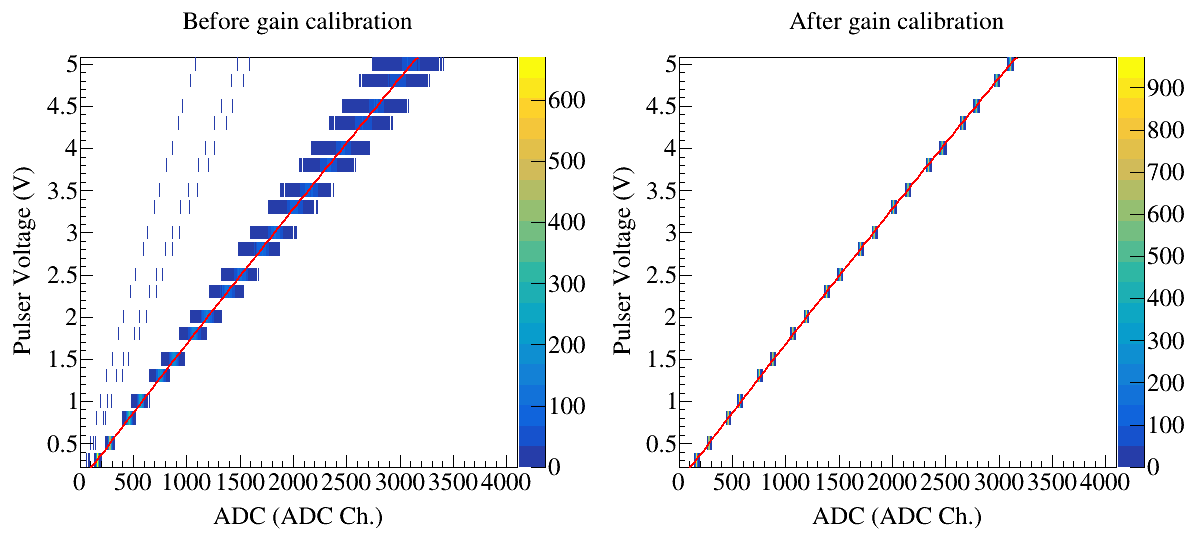
\includegraphics[width=\linewidth]{gaincalib.png}
\caption{Repose of each channel in the electronics to various input voltages of an input signal supplied by a pulse generator.}
\label{fig:gaincalib}
\end{figure}

The electronics were calibrated by measuring the response of each channel to an input signal supplied by a pulse generator. This is a relative calibration technique with the intent to calibrate the varying gains in each channel relative to one another, and not an absolute calibration. The pulse was distributed to all the electronics channels by pulsing the ground plane for a range of input voltages. This distributed the pulse evenly across the entire pad plane. The input voltage is plotted as a function of the measured height of the pulse in the electronics channel given in units of ADC in Fig.~\ref{fig:gaincalib}, for every channel. The small variation in each channel can be seen as the wide band around each measurement point. A linear fit is performed for each channel to get the calibration line for each channel. A channel is chosen which provides a reference calibration to which all other channels are calibrated too. This is done by matching the slopes of each channel to the reference calibration slope.  The right panel shows the resulting distribution of channels after calibration.



\subsection{Anode gain calibration}
\label{sec:anodeCalib}
As discussed in Section~\ref{sec:wireplanes} the voltage of the anode sections 12 and 14 were reduced during the experiment due to high currents being observed on the wires. Out of all the runs used in the analysis in this thesis \ref{tb:runList}, the anode sections 12 and 14 were lowered to \SI{1085}{\volt} for runs 2272-2371 and set to \SI{1214}{\volt} for all the other runs. By lowering the voltage on these anode wires, the gas gain is lowered as compared with all the other anode wire plane sections which operate at \SI{1460}{\volt}. To account for the drop in gain, we increase the gain of the pads which lie above these anode wires  in the software gain of the other channels. The gain factor is found by plotting the energy loss in the high gain sections to the low gain sections.


\begin{figure}[!htb]
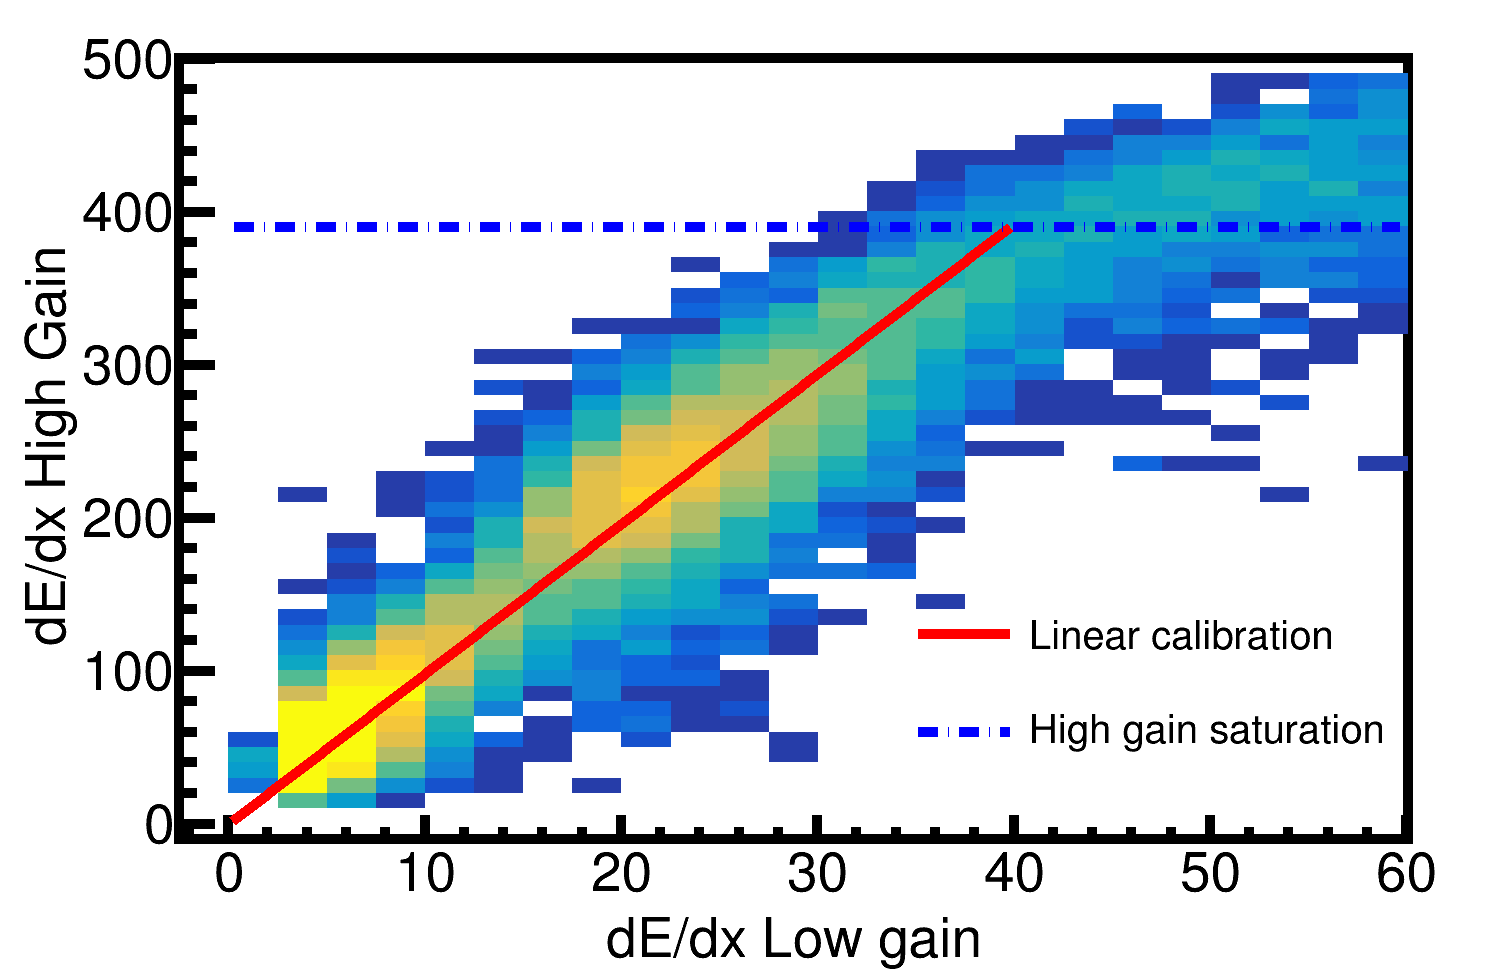
\includegraphics[width=\linewidth]{highlowcal.png}
\caption{Calibration of low and high gain sections of the anode wires.}
\label{fig:highlowcal}
\end{figure}

Figure~\ref{fig:highlowcal} shows the correlation plot of $\langle dE/dx\angle$ of the high versus the low gain sections. The effects of the high gain channel saturation can around a value of 400 ADC\si{\per\milli\metre} and plateaus, where as the low gain does not; this region is left out of the fit. A linear fit was performed for the calibration between the high gain channel $h_c = G\cdot l_c$, where $l_c$ is the value of the low gain channel and $G$ is the gain factor. In the case where the low anode voltage was \SI{1214}{\volt}, the $G=9.8$, where in the case of \SI{1085}{\volt}, the $G = $.  

 A map of the channels which are affected by the low gain and the relevant gain factor was input into the software. In the decoder task the raw ADC spectra was multiplied by the input gain for a given channel. The thresholds of those channels also were multiplied by the same gain factor since the noise levels were also artificially magnified by this method. 

\subsection{Extending the dynamic range of the Electronics}
\label{sec:extendDynamicRange}

Using a TPC for measurements of HIC in nuclear physics presents a different set of challenges as opposed to higher energy experiments. Typically in higher energy experiments fundamental particles are produced with charge $\pm e$. Also, the particles are traveling at higher energies in which the energy losses are near or close to the minimum in the energy loss curve. The dynamic range of most TPC electronics can cover a wide range of particles in these types of experiments. In nuclear HICs, we are interested in measured particles with charges $Ze$ where Z=1-3, and even higher in some applications. The energy loss in the Bethe-Bloch equation, Eq.~\ref{eq:bb}, is proportional to $Z^2$. Even more, low energy nuclear HIC of intermediate beam energies (around \SI{300}{\MeVA}) produce low velocity particles which exist in the $1/\beta^2$ region of Eq.~\ref{eq:bb}, where the energy loss grows dramatically. The dynamic range of electronics significantly limit the PID as the charge of a particle increases and the velocity decreases where the electronics will be saturated.

Several TPCs have tried to address this issue by having regions of low and high gain, either in amplification gain or in electronics gain. This mitigates the complete loss of information but introduces a new problem. Though particles which deposit large amounts of charge will now have good measurements in the low gain areas, particles which deposit minimal energy losses will lose information in the same low gain areas. The reconstruction of such tracks will suffer. There are ongoing efforts in the nuclear community to develop new electronics which hope to mitigate these issues by developing more sophisticated  pre-amplifiers and electronics CITE HERE.  Never the less it is quite useful to develop a software technique which may extend the dynamic range of TPC electronics without the use of new external hardware, especially for experiments which have already been performed with older electronics technologies. In this section we will outline a novel software technique that takes advantage of the PRF described in Section~\ref{sec:prf} and can effectively extend the dynamic range of the TPC electronics. 

In TPCs, the effective dynamic range is very different from the single channel dynamic range depending on how the TPC measurement is used. Typically TPCs are operated inside of a magnetic field for the purpose of reconstructing the momentum of a track, which requires sub-millimeter precision in the position determination of the track path. This is achieved by clustering several pads together as discussed in Section~\ref{sec:helixtrack}. To achieve this at least 2 adjacent pads must be measured, and the precision increases as the number of adjacent pads increases. 

The effective dynamic range is then not the single channel dynamic range, but the dynamic range between central pad --holding the largest charge-- and the adjacent pads --holding the smaller charges in the PRF distribution. For example, to measure minimum ionizing particles, the Signal-to-Noise-Ratio (SNR) of the pad with the smallest charge in the distribution should be some reasonable value above noise, so that the signals can be measured. From the PRF in Section~\ref{sec:prf}, we know the central pad in the cluster holds 80\% of the total charge, where as the two adjacent pads each hold the remaining 10\%. In the \spirit TPC the electronics gain was set so that the the pads have a SNR of 6:1 for minimum ionizing tracks, and therefore the central pad had a SNR of 50:1. In the case of the maximum charge is collected in the central pad, before the electronics saturate, the SNR is 800:1. Therefore the maximum SNR is roughly 16 times that  --800 over 50 -- of minimum ionizing particles. This is order to have a complete measurement, where adjacent pads are all measured and position resolution is not compromised. 

Figure~\ref{fig:intro} shows the theoretical energy loss curves for several particles as a function of the momentum over charge. Minimum ionization can be seen to take place around \SI{10}{\kilo\electronvolt\per\centi\metre}. The dashed lines and vertical blue bar in are separated by a factor of 16, representing the effective dynamic range in the \spirit TPC. This dynamic range should be regarded as approximate because the energy loss fluctuates significantly about the most probable energy loss as described in Section~\ref{sec:energyloss}. Nevertheless, the blue dashed lines and vertical blue bar illustrate that the range of energy losses sampled in a fixed gain readout system is limited. One can change the gain and shift the energy loss range that can be sampled, but the dynamic range itself cannot be increased.

  
\begin{figure}[ht!]
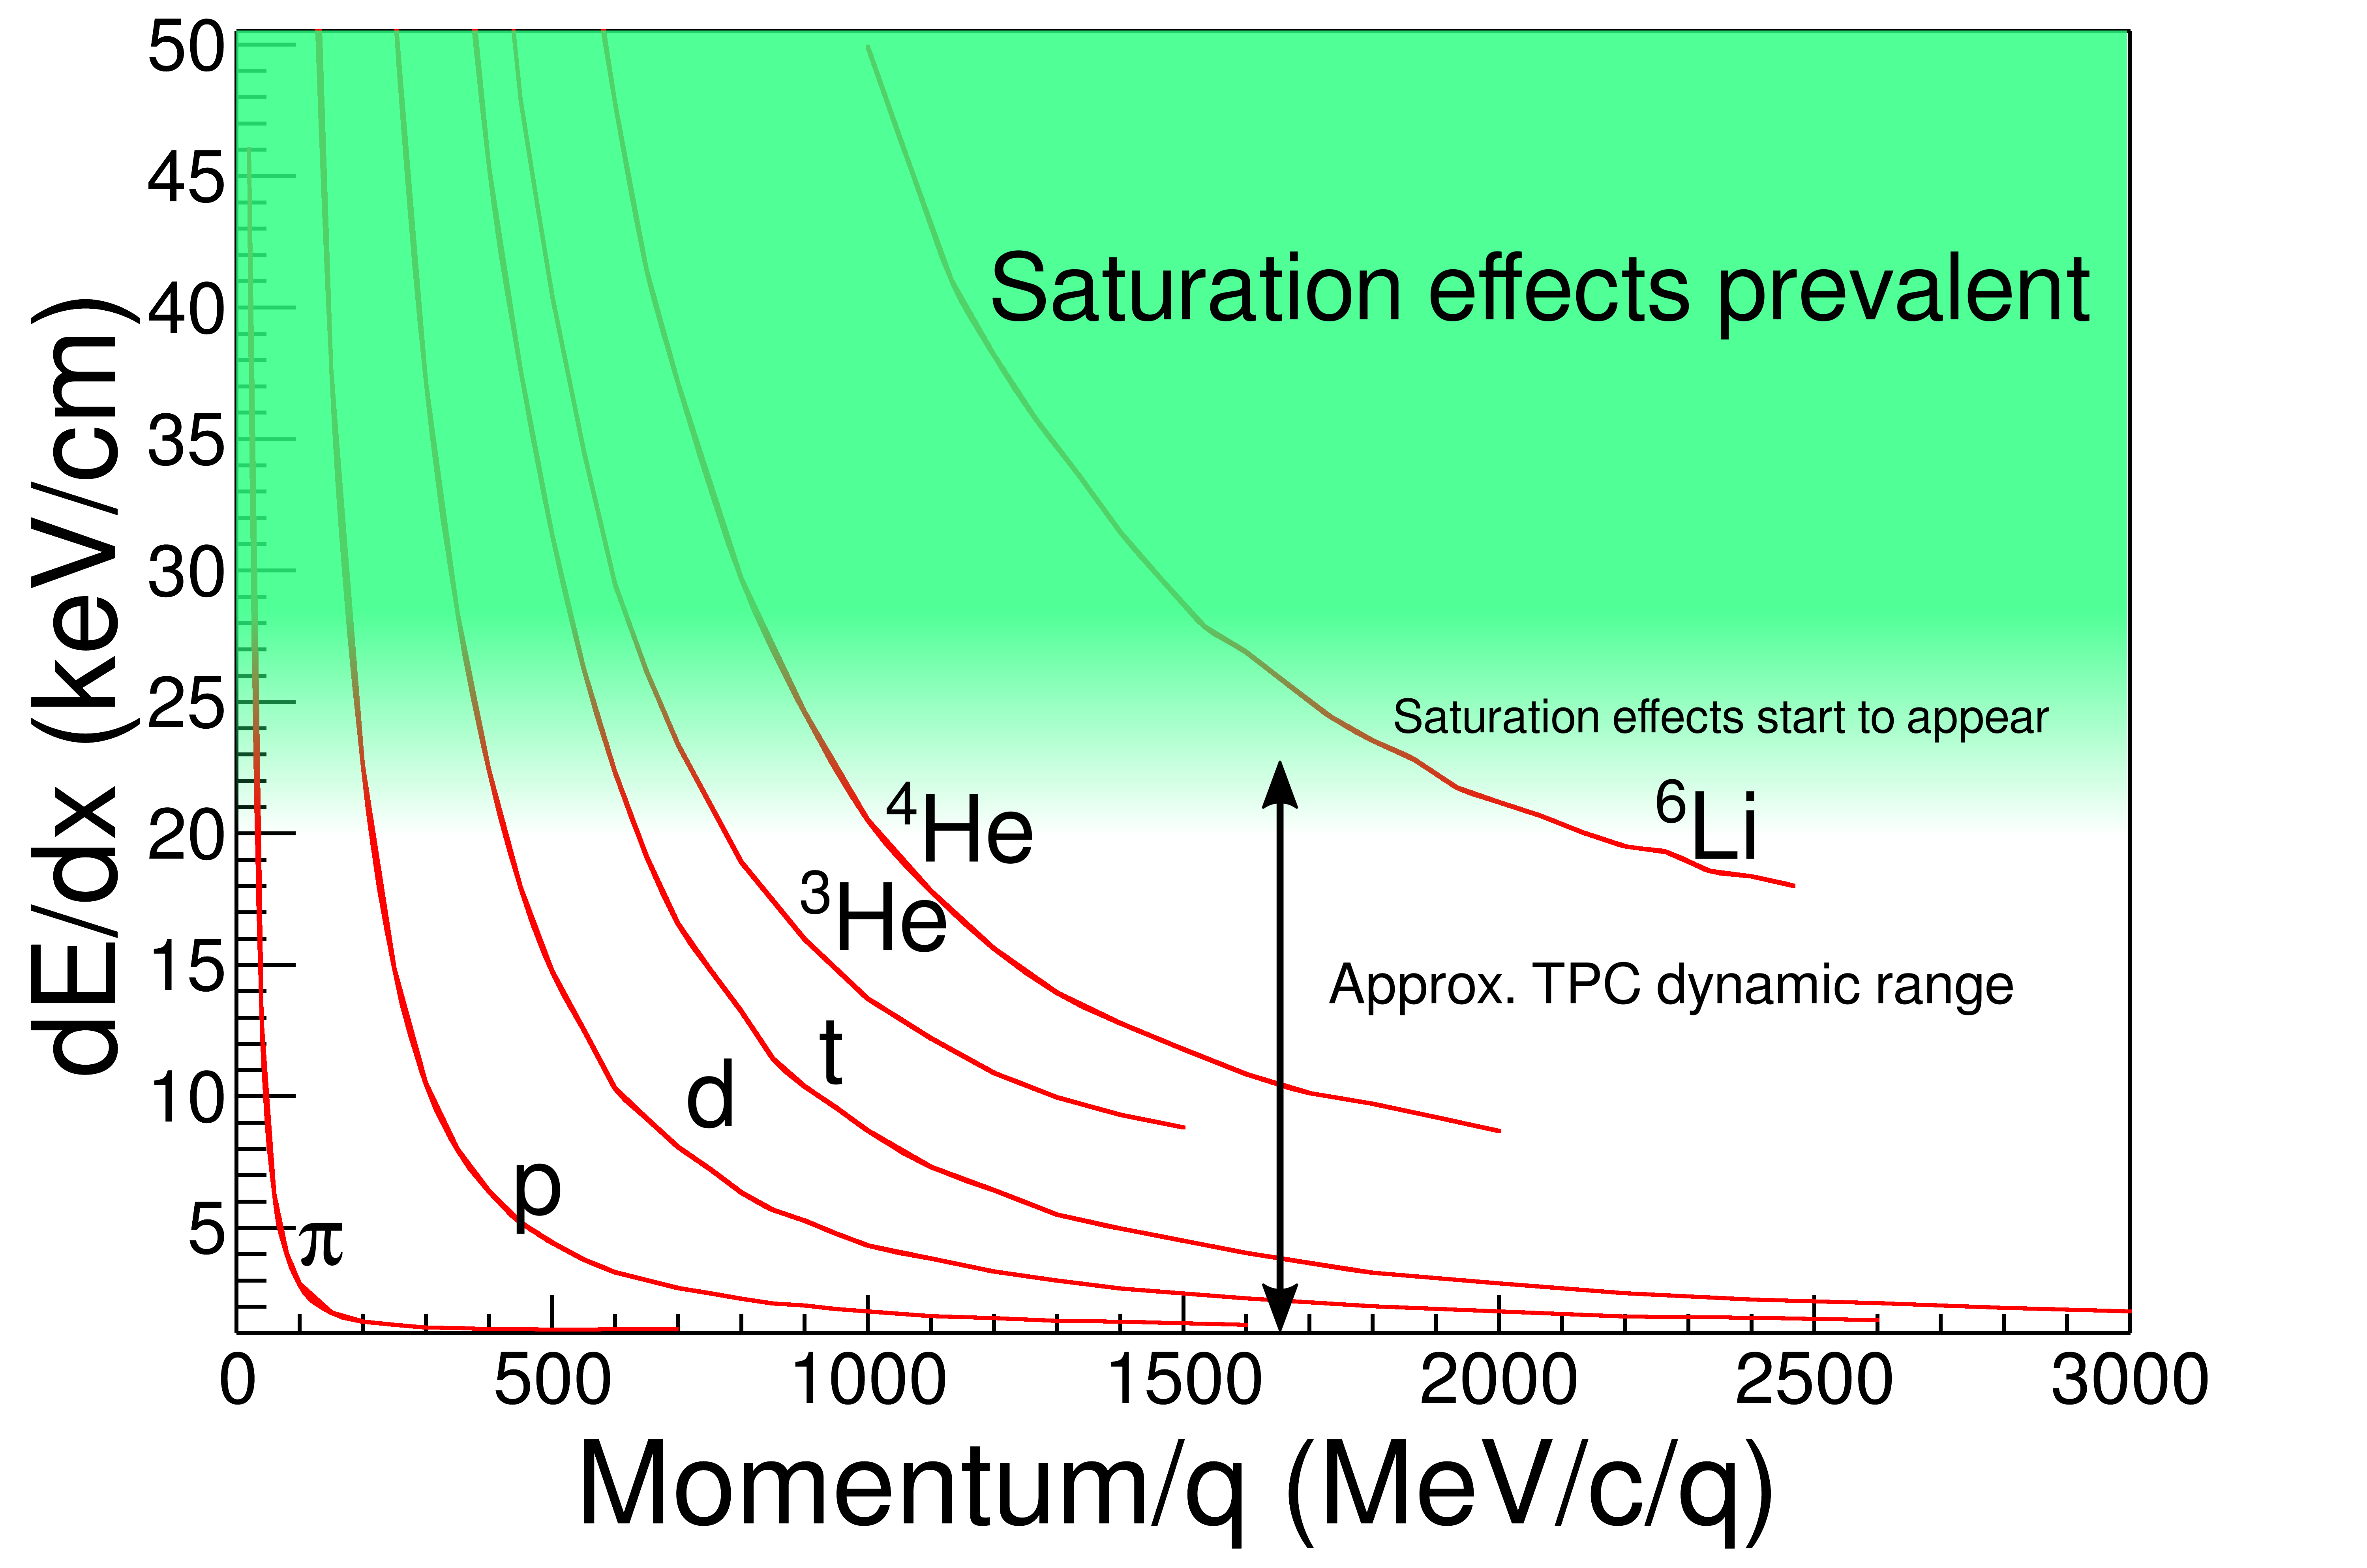
\includegraphics[width=\linewidth]{intrographic}
%\includegraphics[width=\linewidth]{intrographic_2}
\caption{The expected $dE/dx$ lines of different particles are given in red as calculated by Geant4. The approximate dynamic range of the TPC is shown by the vertical bar for the gain setting used in the experiment. Anything outside of this region would be saturated to some degree.}
\label{fig:intro}
\end{figure}


\subsection{Experimental Pad Response Function}
\label{sec:expPRF}
The pad response function of the TPC was extracted from non-saturating hits and clusters in tracks at various track crossing angles. As in Fig.~\ref{fig:topview}, we postulate that the PRF is a function of the total charge deposited in a cluster $Q = \sum_i q_i$, and the difference in position of the center of the $i^{th}$ pad, $x_i$, to the mean position $\bar{x} = \sum_i x_i q_i/Q$, defined as $\lambda_i = x_i-\bar{x}$. The PRF is simply defined as the charge fraction of each pad as a function of $\lambda$, as shown in Equation \ref{eq:prf}. 

\begin{equation}\label{eq:prf}
PRF(\lambda_i) = \frac{q_i(\lambda_i)}{Q}
\end{equation}

Averaging over many events in the experimental data, the resulting PRF for the S$\pi$RIT TPC is shown in Fig.~\ref{fig:expprf}. Here we see the deviations from the expected analytic Gatti distribution (black curve), whereas fitting with a two parameter Gaussian function (red curve) gives a better description of the data, Eq.~\ref{eq:gaus}, with the two parameters being the normalization coefficient, $N_0$, width $\sigma$.

\begin{equation}\label{eq:gaus}
PRF_{\mathrm{Gaus}}(\lambda) = N_0 e^\frac{-\lambda^2}{2\sigma^2}
\end{equation}

\begin{comment}
\begin{figure}[ht!]s
\begin{overpic}[width=\linewidth]{fig5.pdf}
\put(61,55){\contour{white}{ PRF${}_{\mathrm{Gaus}}(\lambda)$ eq. \ref{eq:gaus}  }}
\put(61,49){\contour{white}{ PRF${}_{\mathrm{Gatti}}(\lambda)$ eq. \ref{eq:gatti} }}
\end{overpic}
\caption{Experimental pad response function of many events for a crossing angle of $85^{\circ} < \theta \leq 90^{\circ}$.  }
\label{fig:expprf}
\end{figure}
\end{comment}


The shape of the PRF depends on the crossing angle of the track, which determines how wide the charge is distributed along the wire \cite{gatti}. Figure~\ref{fig:prfpimData} shows the PRF for $\pi^-$ tracks versus the crossing angle $\theta$ of the track. The PRF gets wider starting from $90^{\circ}$  and until where we switch clustering directions at $\ang{45}$. If we did not switch clustering directions the PRF would become wider until it was a uniform distribution and there was no position resolution. Switching from $x$ to the $z$ direction clustering the opposite trend is seen where the PRF becomes narrower  going from $45^{\circ}$ to $0^{\circ}$, as the position resolution gets better.

\begin{figure}[!htb]
     \centering
	 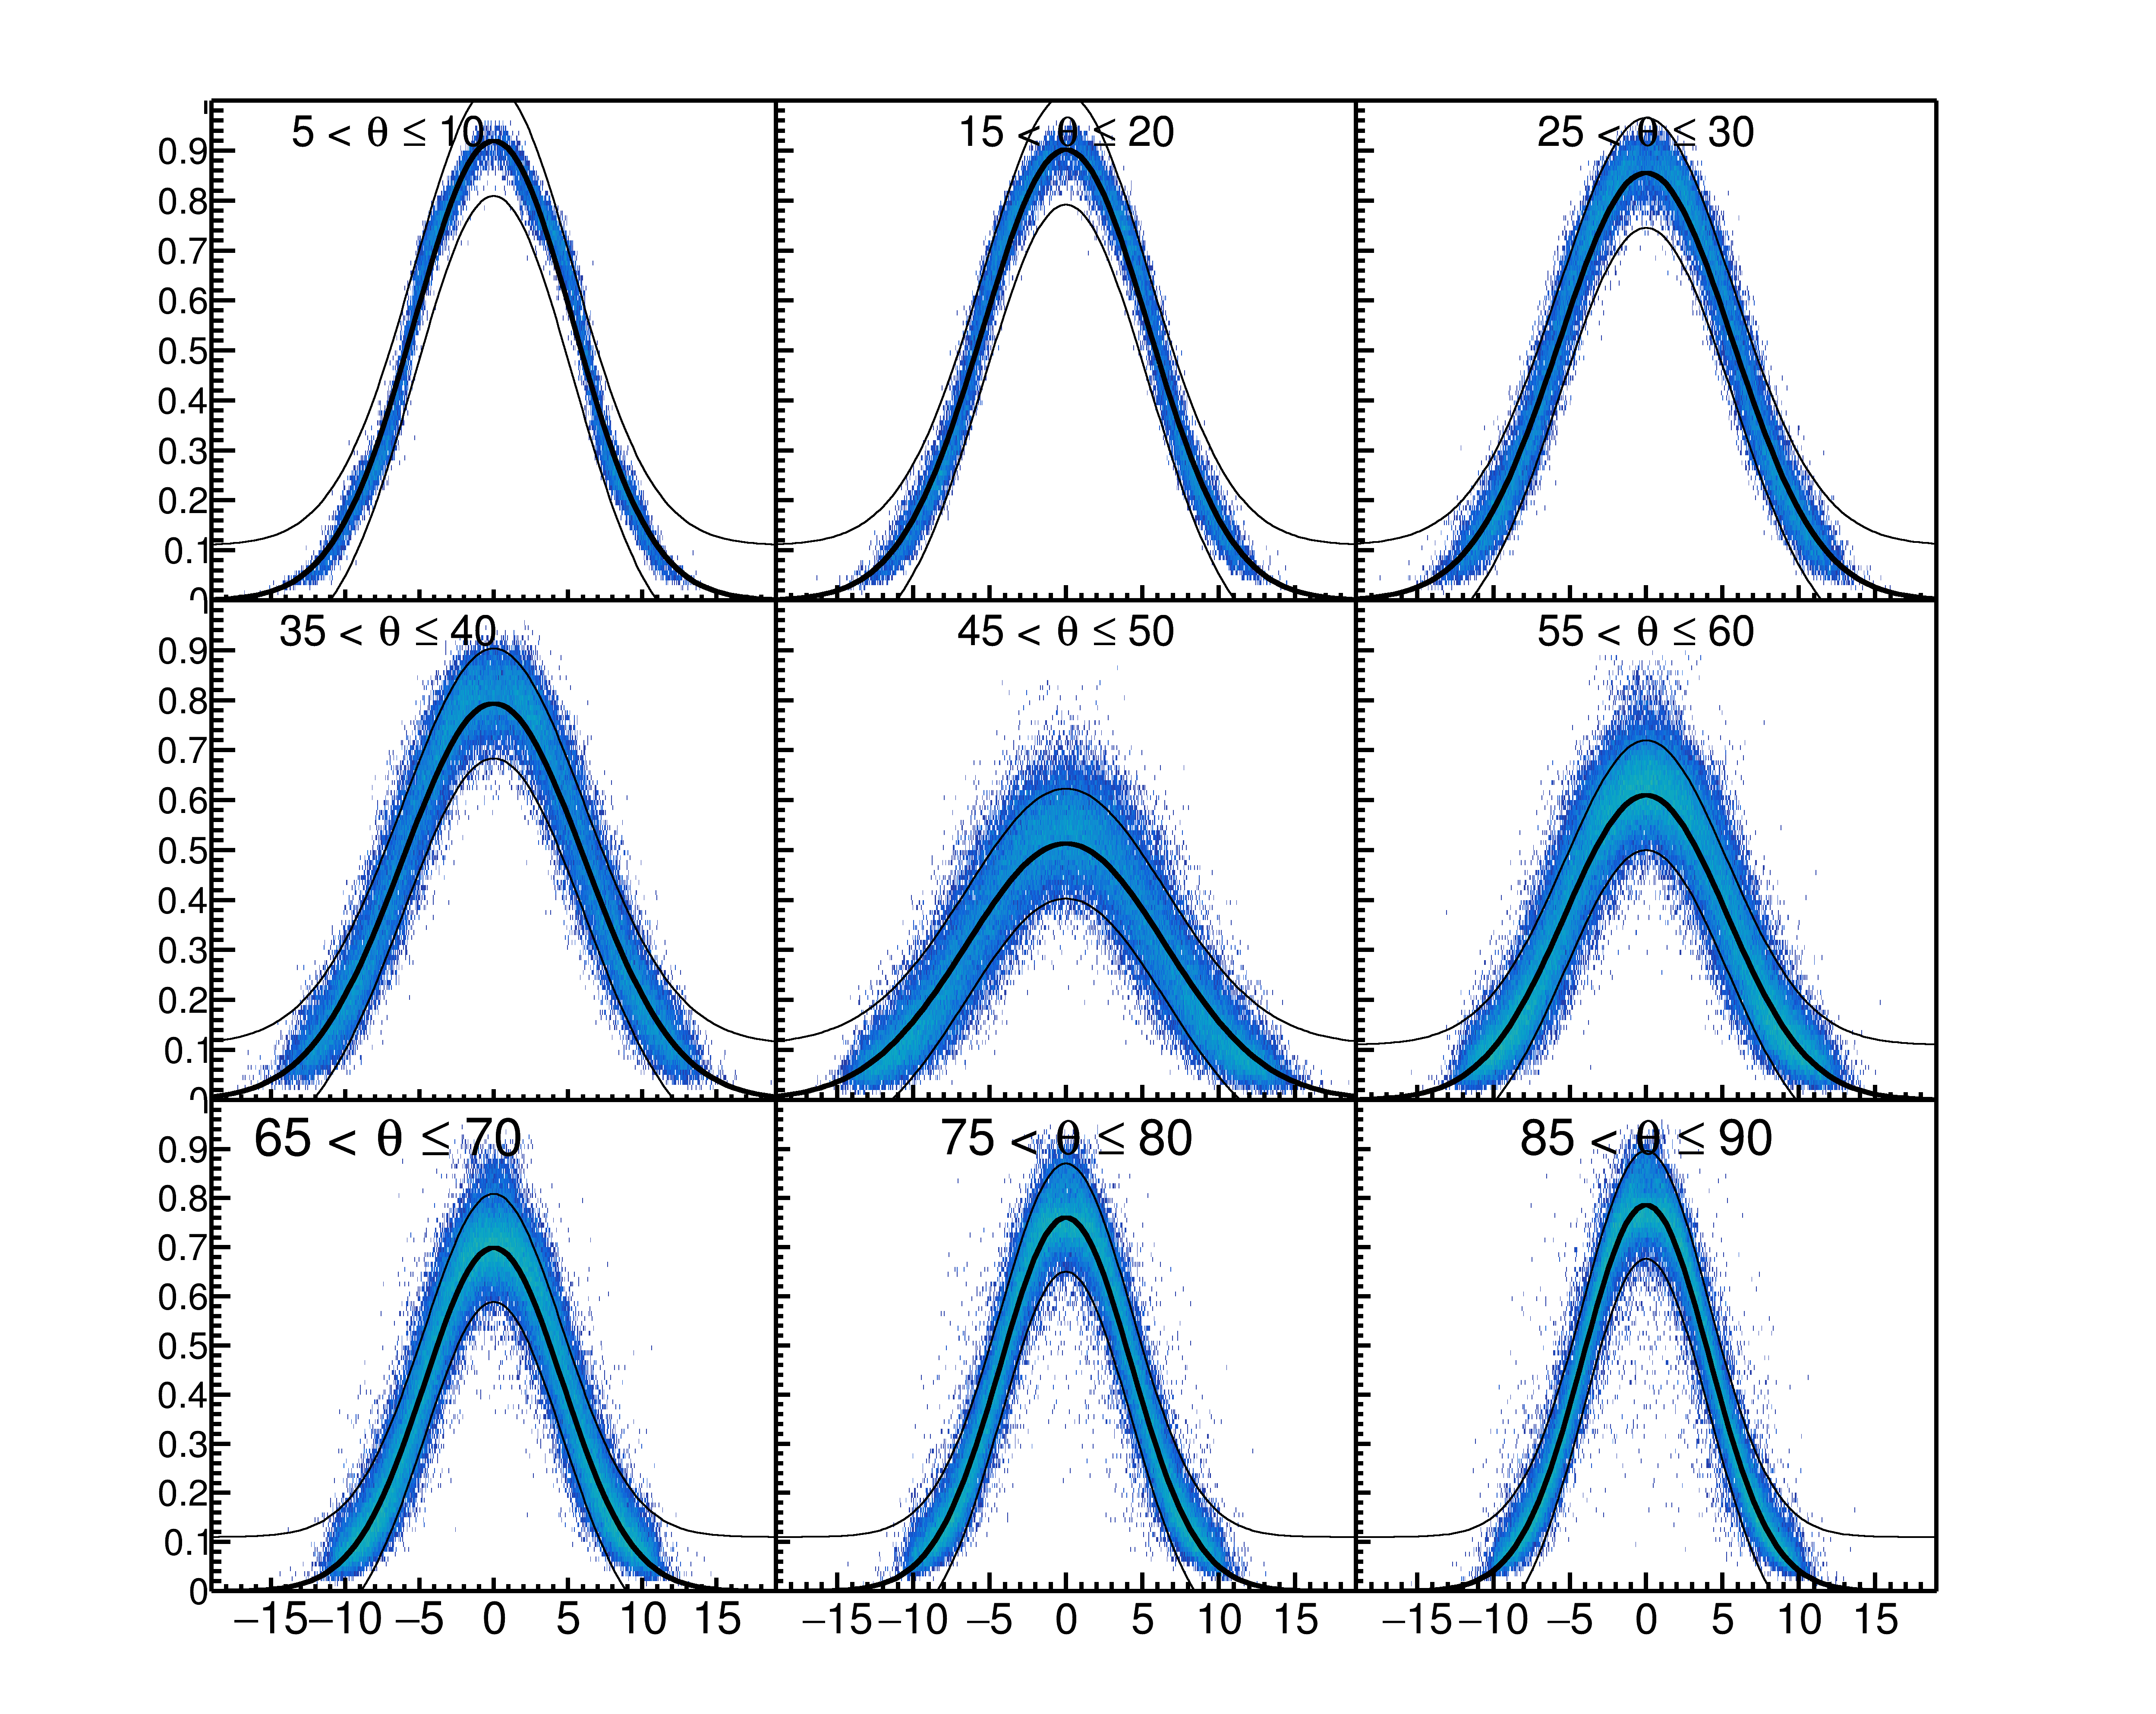
\includegraphics[width=\textwidth]{PRFs_data_wcut.png}
     \caption{PRF from $\pi^-$ tracks in experimental data. }
     \label{fig:prfpimData}
\end{figure}

\begin{figure}[ht!]
\vspace{5mm}
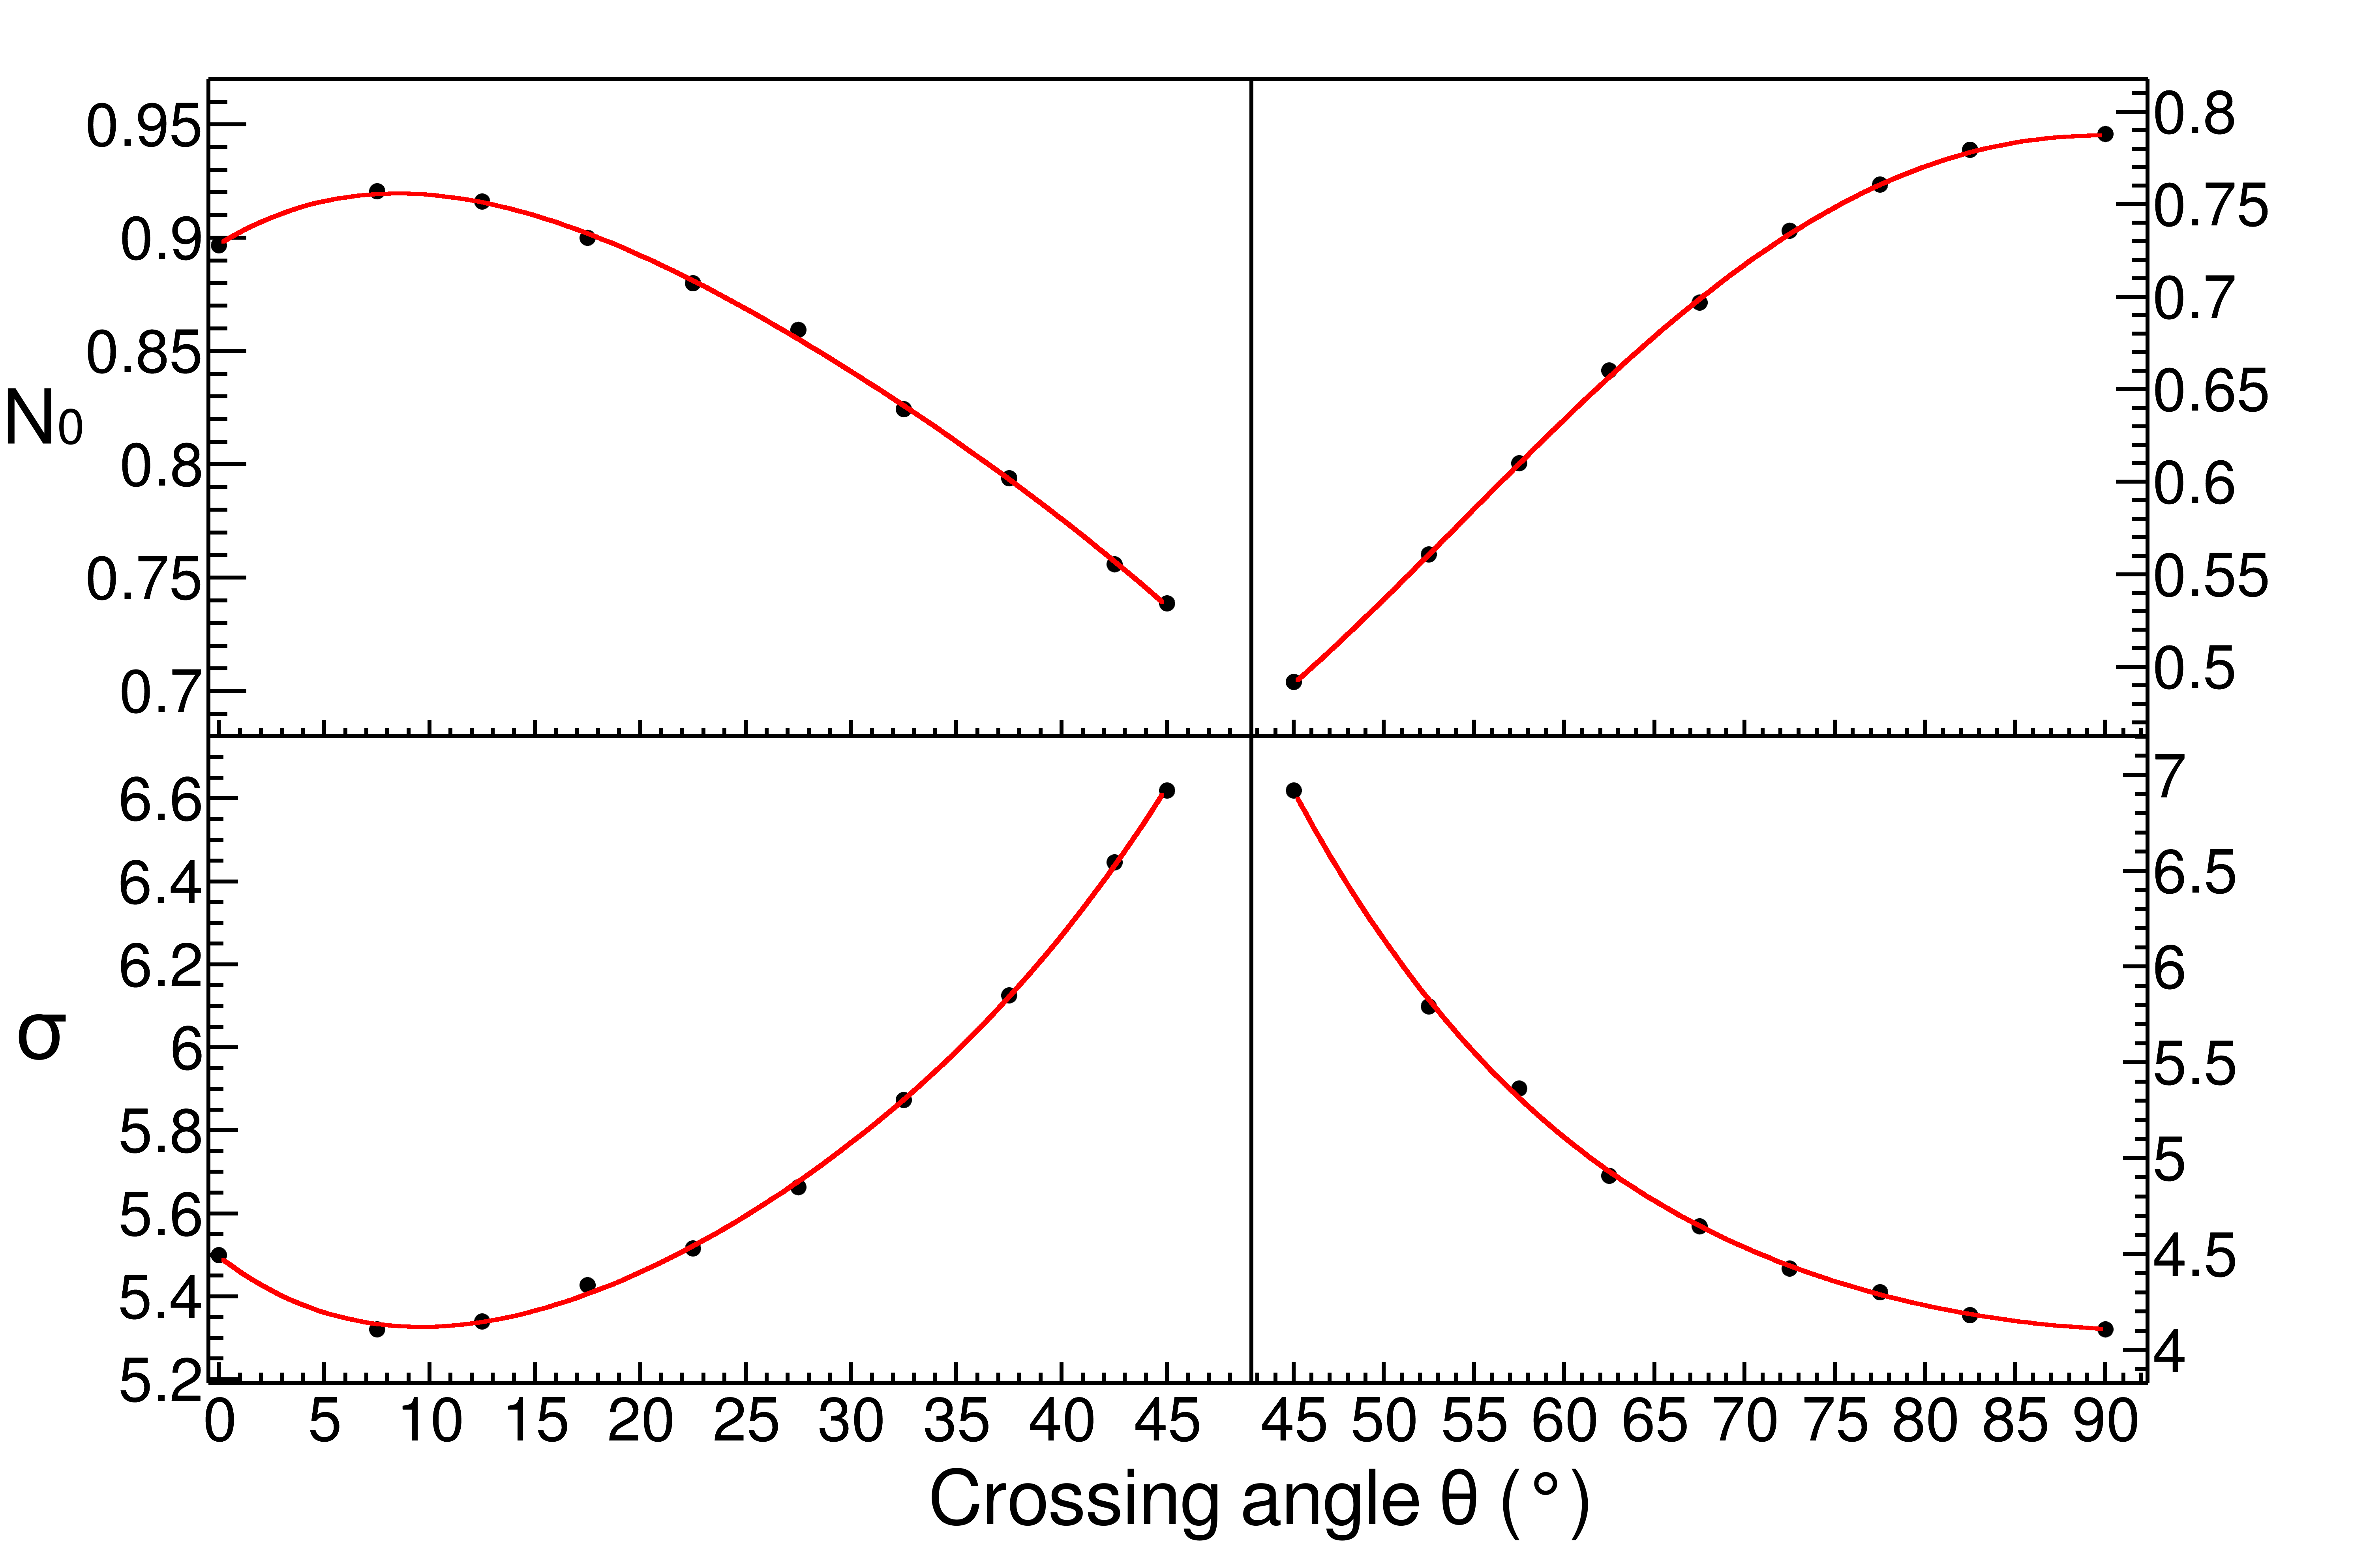
\includegraphics[width=\linewidth]{fig7}
\caption{Parameters $N_{0}$ and $\sigma$ as a function of the crossing angle $\theta$ with the $4^{th}$ order polynomial fits.}
\label{fig:normsigma}
\end{figure}

\begin{comment}
\begin{table}
\centering
 \begin{tabular}{||c c c c c c||} 
 \hline
 Coefficient & $c_0$ & $c_1$ & $c_2$ & $c_3$ & $c_4$ \\ [0.5ex] 
 \hline\hline
 $0 < \theta < 45$ & & & & &  \\ [.25ex]
 \hline
 $N_0$ & .897 & 5.766E-3 & -4.263E-4 & 7.444E-6 & 5.705E-8 \\ 
 \hline
 $\sigma$ & 5.496 & -3.920E-2 & 2.693E-3 & -5.208E-5 & 5.334E-7\\
 \hline
 $45 < \theta < 90$ & & & &  & \\ [.25ex]
 \hline	
 $N_0$ & 1.220 & -6.258E-2 & 1.608E-3 & -1.492E-5  & 4.654E-8 \\
 \hline
 $\sigma$ & 31.368 & -1.109 & 1.779E-2 & -1.336E-4 & 3.940E-7\\
 \hline
\end{tabular}
\caption{Coefficients of the $4_th$ order polynomial fit to the Gaussian parameters $N_0$ and $\sigma$. The polynomial form is given as $c_0 + c_1 x + c_2 x^2 + c_3 x^3 + c_4 x^4$}
\label{tb:coeff}
\end{table}
\end{comment}
 
A Gaussian fit was performed to the experimental PRF in $\ang{5}$ width bins ranging from $\ang{0} < \theta \leq \ang{90}$. Figure~\ref{fig:normsigma} shows the two parameters resulting from fitting the the Gaussian function given in Eq.~\ref{eq:prfgaus} which are are plotted versus $\theta$. A $4^{th}$ order polynomial fit of these parameters allowed for interpolating for any given $\theta$ value, which is shown as the black line. 


\subsection{Method of Desaturation}
\label{sec:desat}

\begin{figure}[ht!]
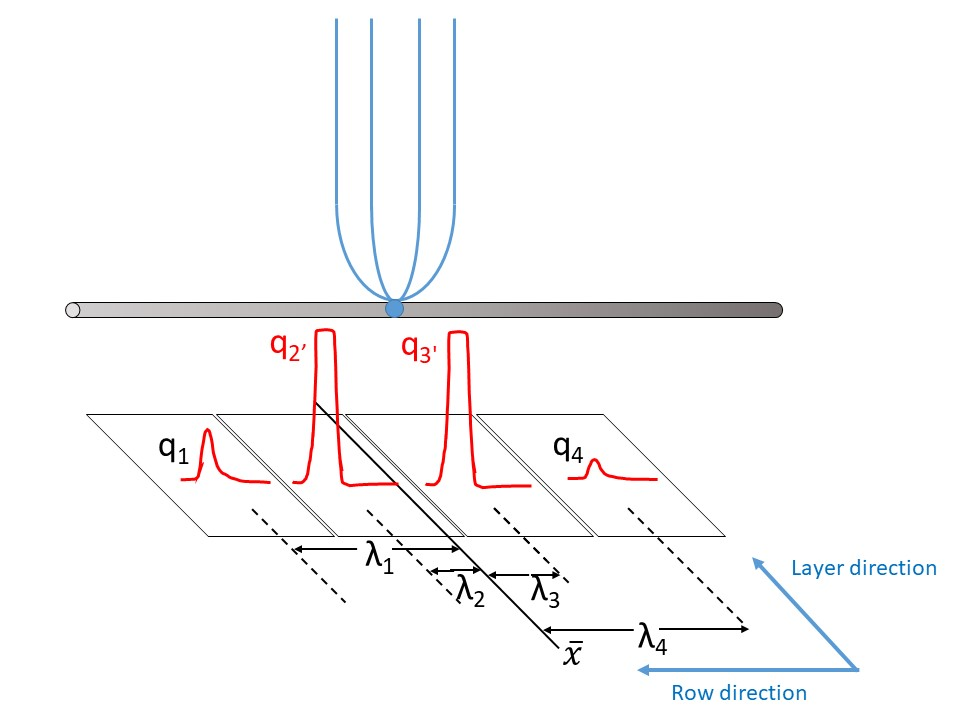
\includegraphics[width=\linewidth]{saturated_pads}
\caption{A typical case of a saturating event. The red pulses represent the time bucket signal for each collected charge. The pads directly underneath the avalanche point, $q_{2'}$ and $q_{3'}$, are saturated while pads farther away, $q_1$ and $q_4$ are not saturated.}
\label{fig:satpad}
\end{figure}

In the following, we will use the term ``desaturation'' to describe the technique described here of correcting the charge values of the saturated pads. Figure~\ref{fig:satpad} shows a typical situation of saturated hits in a cluster. When an avalanche causes a large enough induced signal, the pads directly underneath the avalanche collect the largest charge becoming saturated, denoted here as $q_{2\textprime}$ and $q_{3\textprime}$. Pads further away collect less charge and typically are not saturated, detonated here as $q_{1}$ and $q_{4}$. Though the charge values in the saturated channels are lost, we know that the distribution of all charges must follow the PRF which is a fixed function, and a fundamental operating principle of all TPCs. We have already measured the PRF as a function of crossing angle in Section~\ref{sec:expPRF}, and from the tracking information, we know the crossing angle of the track at a given cluster and therefore the PRF corresponding to that cluster. 

We assume the distance of each pad to the track, $\lambda_i$, is fixed, defining the fraction of charge each pad receives as defined by the $PRF(\lambda_i)$ function. To determine the best estimate for the charge values of each saturated pad, a chi squared function is minimized,

\begin{equation}\label{eq:chi}
\chi^2 = \sum_i \frac{(q_i^{\mathrm{obs}} - q_i^{\mathrm{expect}})^2}{q_i^{\mathrm{expect}}},
\end{equation}


where $q_i^{\mathrm{obs}}$ are the non-saturated charges and $q_i^{\mathrm{expect}}$ are the charge values expected for that pad as calculated from the PRF; $q_i^{\mathrm{expect}} = Q\cdot PRF(\lambda_i)$. The saturated charge values $q_{i}^{\textprime}$ are treated as unknown variables and are allowed to vary in the $\chi^2$ minimization, they enter the minimization routine when they are added to get the total charge $Q = \sum q_i + \sum q_i^{'}$. 


\begin{figure*}[!htb]
\centering
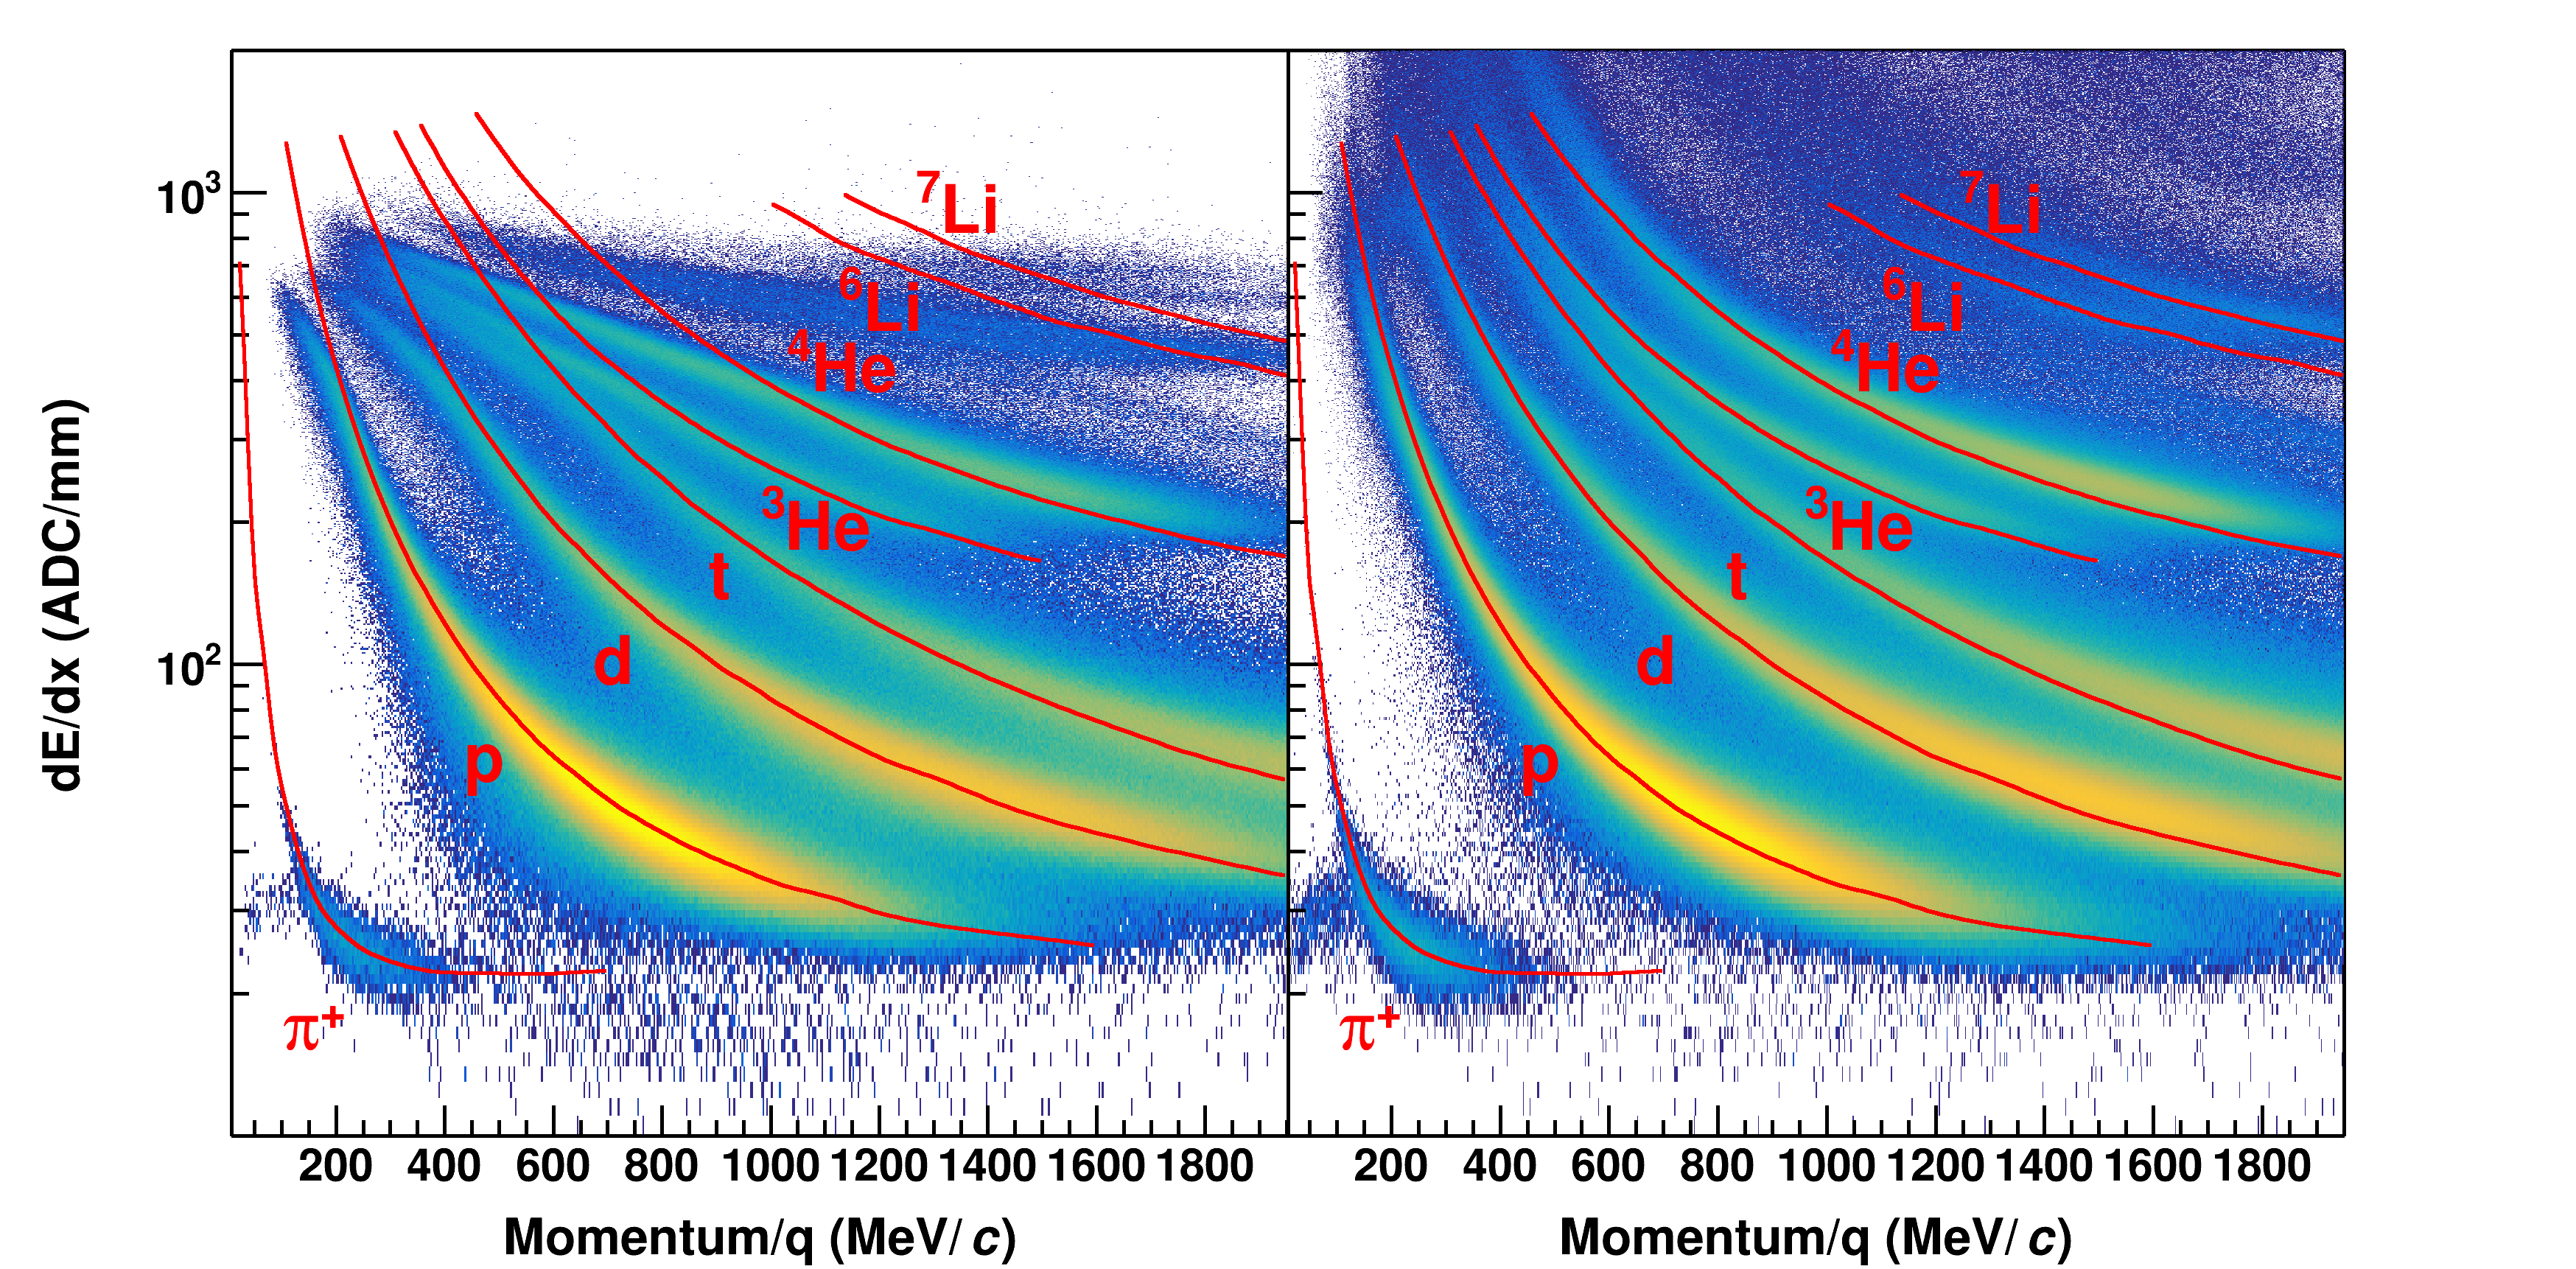
\includegraphics[width=\linewidth]{data_combine}
\caption{Uncorrected (left panel) and desaturated (right panel) collision data at polar angles of $\theta < 40^{\circ}$ and azimuthal angles between $-80^{\circ} < \phi < 80^{\circ}$}
\label{fig:data_combine}
\end{figure*}


\begin{figure*}[!htb]
\centering
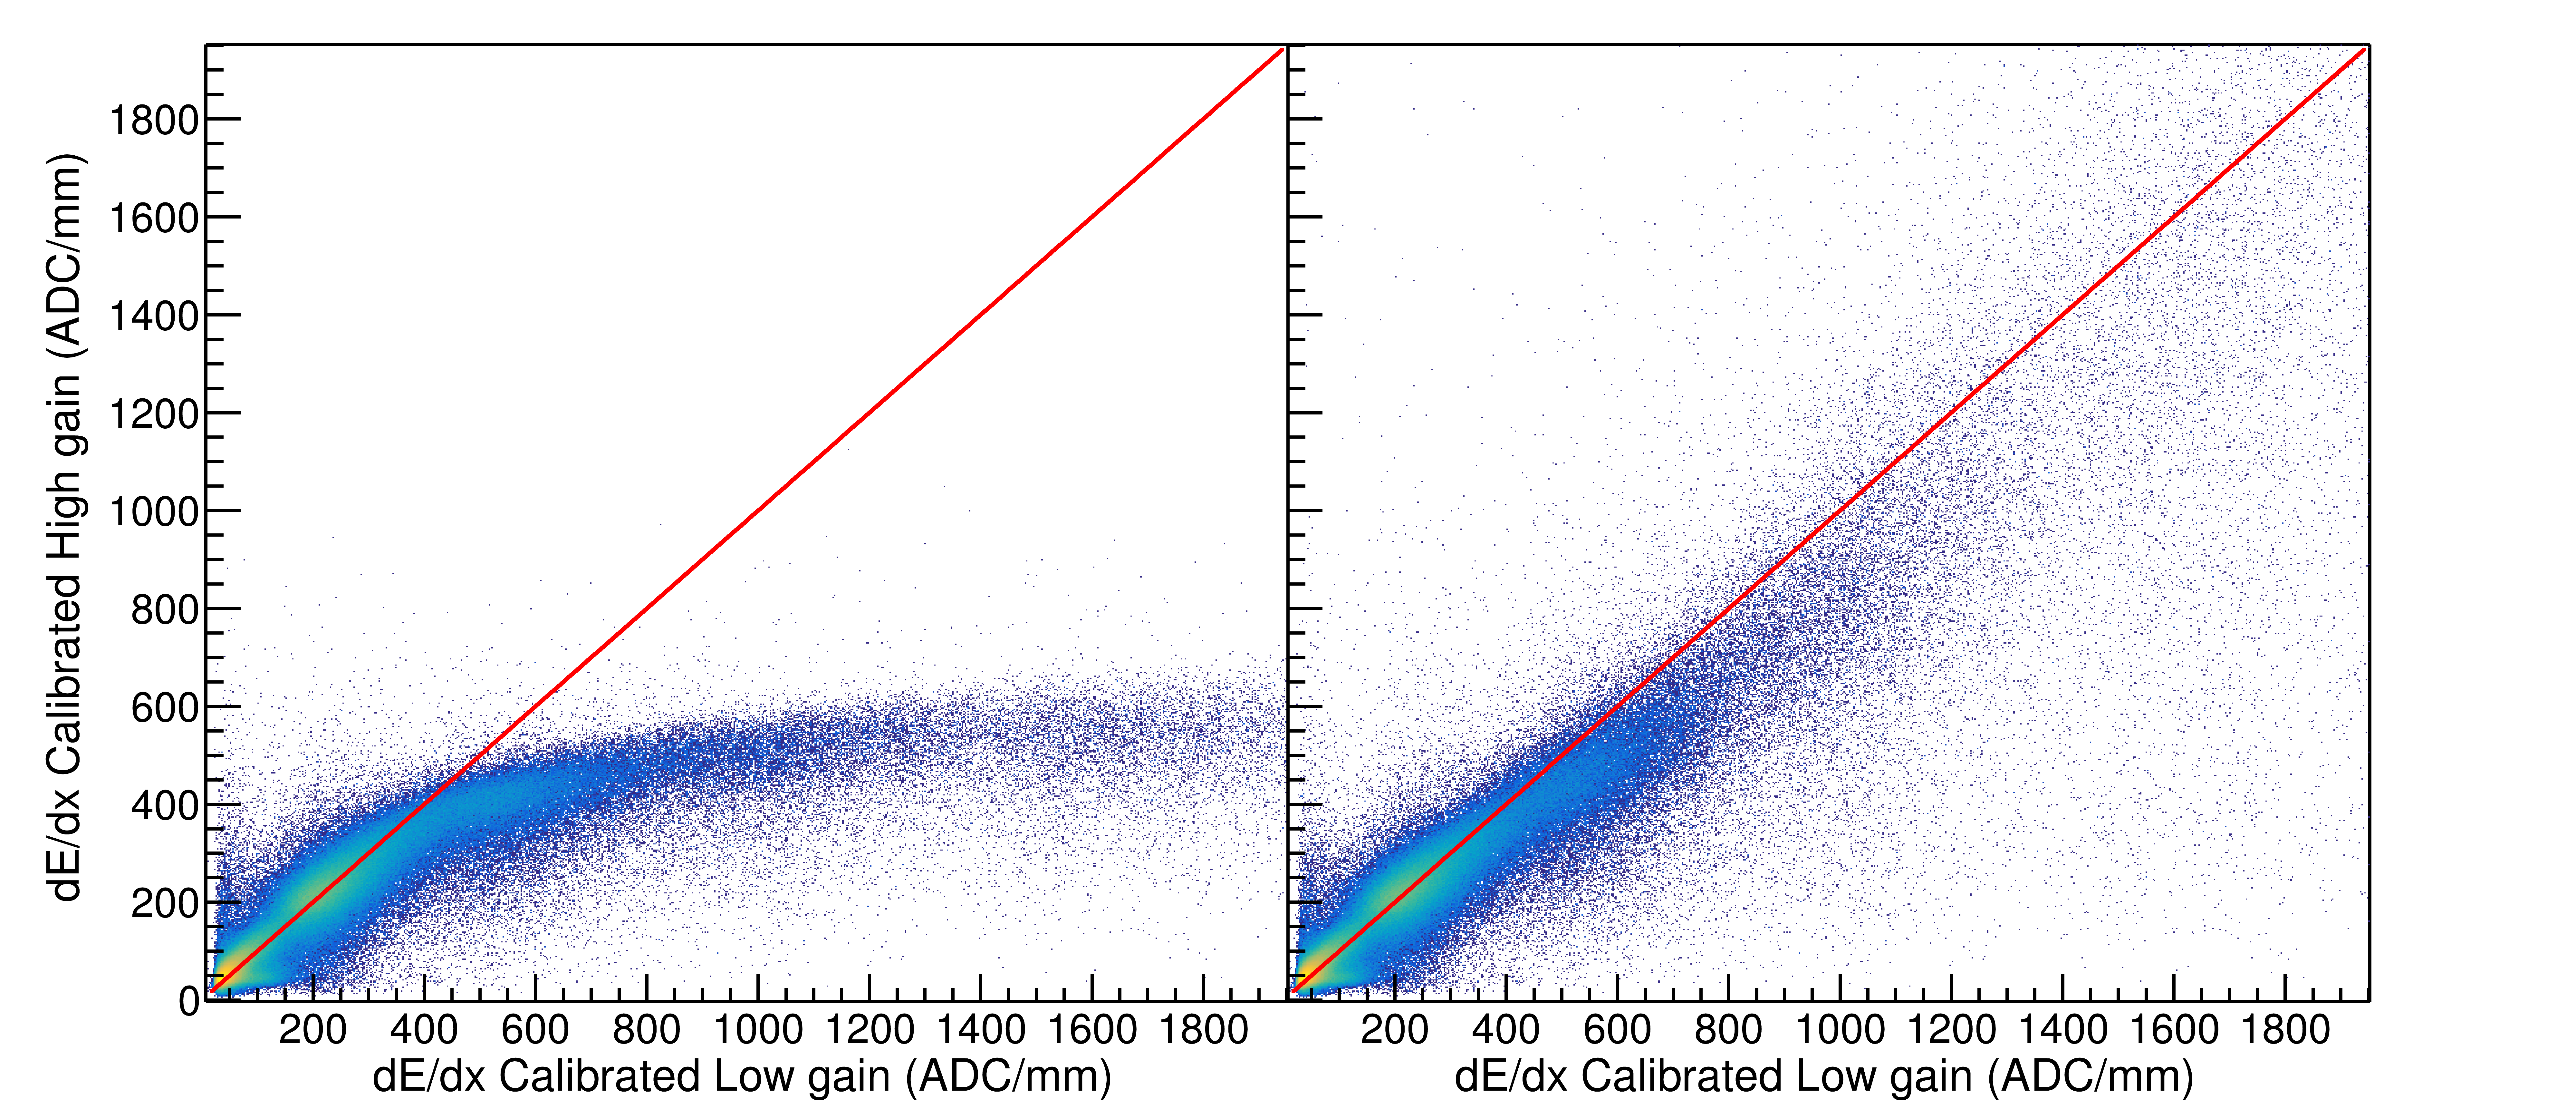
\includegraphics[width=\linewidth]{lowvshigh.png}
\caption{Uncorrected (left panel) and desaturated (right panel) collision data comparing the low gain region to the high gain anode regions of the TPC.}
\label{fig:lowvshigh}
\end{figure*}

Tracks which saturate pads in the high anode wire voltage region are not saturated in the low anode voltage region. By comparing the $\langle dE/dx\rangle$ values of these two sections. While this desaturation technique avoids the need to lower the gain of any region, the low anode voltage region proved to be a direct measurement of the success of this technique.
 
Figure~\ref{fig:lowvshigh} shows the the $\langle dE/dx\rangle$ values of the high gain region compared with the calibrated low gain region. The effect of saturation can be seen in the high gain region for the uncorrected data above values of 400 ADC/mm where the values plateau, where as the low gain region still returns accurate values. Below this value the electronics are not saturated, and therefore the high and low gain sections agree. After applying the desaturation method, the correlation between the high and low gain sections is restored, as seen in Fig.~\ref{fig:lowvshigh}. From this comparison, we can approximate that the correction has corrected the high gain sections to agree with low gain sections to values of 2000 ADC/mm, increasing the dynamic range by a factor of at least 5.

The success of the desaturation becomes more clear when looking at the particle identification (PID) lines from the experimental data in Fig.~\ref{fig:data_combine}. In the following PID plots the red lines represent the most probable energy loss as given by Geant4 straggling functions. The uncorrected data in the left panel shows the effects of saturation, where the PID lines deviate significantly from their theoretical expectations starting at around 400~ADC/mm. After applying the desaturation technique -- in the right panel-- we see a large improvement, most notably for the He and Li particles, which suffer the most from saturation. Even the ${}^{6}Li$ and ${}^{7}Li$ particles can be separated and a more subtle improvement of the lighter particles, (p, d, t), can also be seen in the PID lines at lower momenta. In these regions, there was little to no PID resolution before desaturation technique was applied.  


%Give some failures of the assumptions made

\subsection{Space Charge Corrections}
\label{sec:spacecharge}

%MAYBE ADD A LITTLE NAPKIN CALCULATION OF SPACE CHARGE TO SHOW ORDER OF EFFECT. 

As the beam passes through the field cage it ionizes the gas creating electron-ion pairs. The drift velocities of the ions are typically \SI{e4} times slower than electron drift velocities \cite{blumrol}. Any source of ions have the potential to build up in the drift volume, creating a positive space charge, distorting the drifting electrons and  biasing the track momentum measurement. There are several regions of the TPC in which ions are created. The largest source of positive ions is created in the avalanche process near the anode wires. But as discussed in Section~\ref{sec:wireplanes}, the gating grid captures all of the ions from this region. The other source of ions come from the primary ionization produced by the beam and reaction products in the detector gas. The energy loss  $\langle dE/dx\rangle \propto Z^2$, where Z is the charge of the particle type. Because the charge of the un-reacted beam is around Z~50, the ionization due to the beam is a factor of \num{2e3} times that of the light charged particles which mostly are of charge Z~1. Therefore the ions resulting from the un-reacted beam is the largest source of positive ions in the TPC. 


NEED TO PUT IN ABOUT THE GATING GRID LEAK 
 
 \begin{comment}
 
 \begin{table}[!htb] % not just 'h!'
\centering % not a center environment
\begin{tabular}{
  @{}
  l
  S[table-format=1.2]
  S[table-format=1.2]
  S[table-format=1.2]
  S[table-format=5.2]
  S[table-format=5.2]
  @{}
}
\toprule
Beam Energy Loss  &
 {${}^{132}$Sn} &
 {${}^{124}$Sn} &
 {${}^{112}$Sn} &
 {${}^{108}$Sn} &
  {Avg.}\\
  
\midrule
$\si{\kilo\eV\per\centi\meter}$ & 11.2   &.034  &5.43   &  903   &150     \\
\bottomrule
\end{tabular}

\caption{Average energy loss of each beam.}
\label{tb:beameloss}
\end{table}
\end{comment}


\begin{figure}[!htb]
\centering
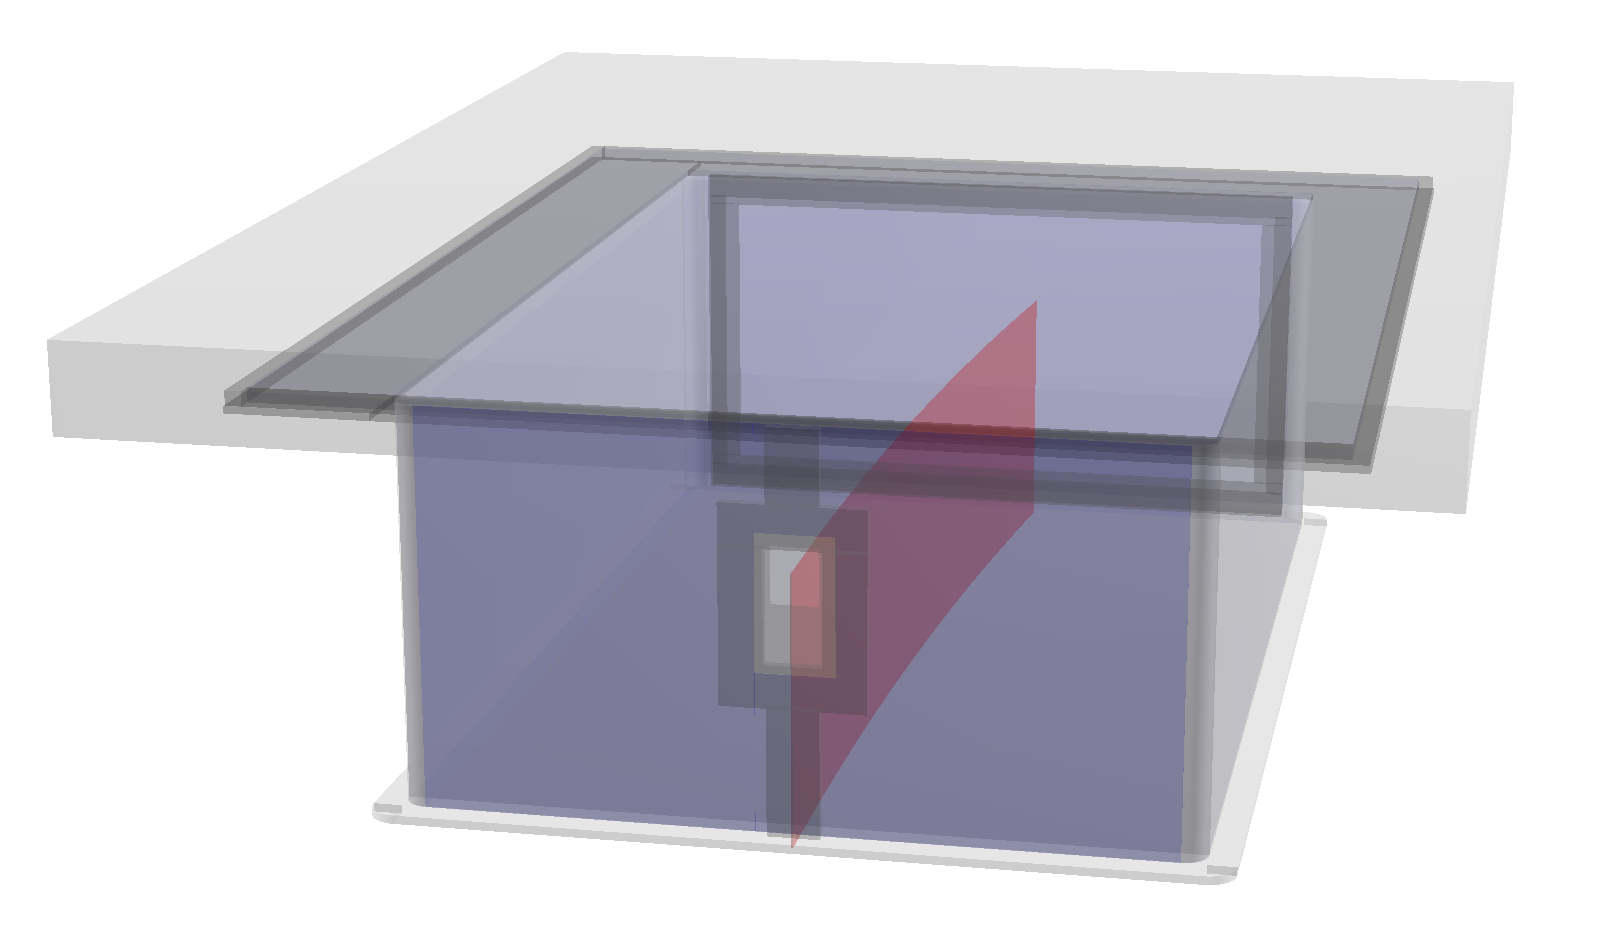
\includegraphics[width=\linewidth]{spacechg_cartoon.png}
\caption{Location of space charge in 132 Sn}
\label{fig:spacechg_cartoon}
\end{figure}


\begin{figure}[!htb]
\centering
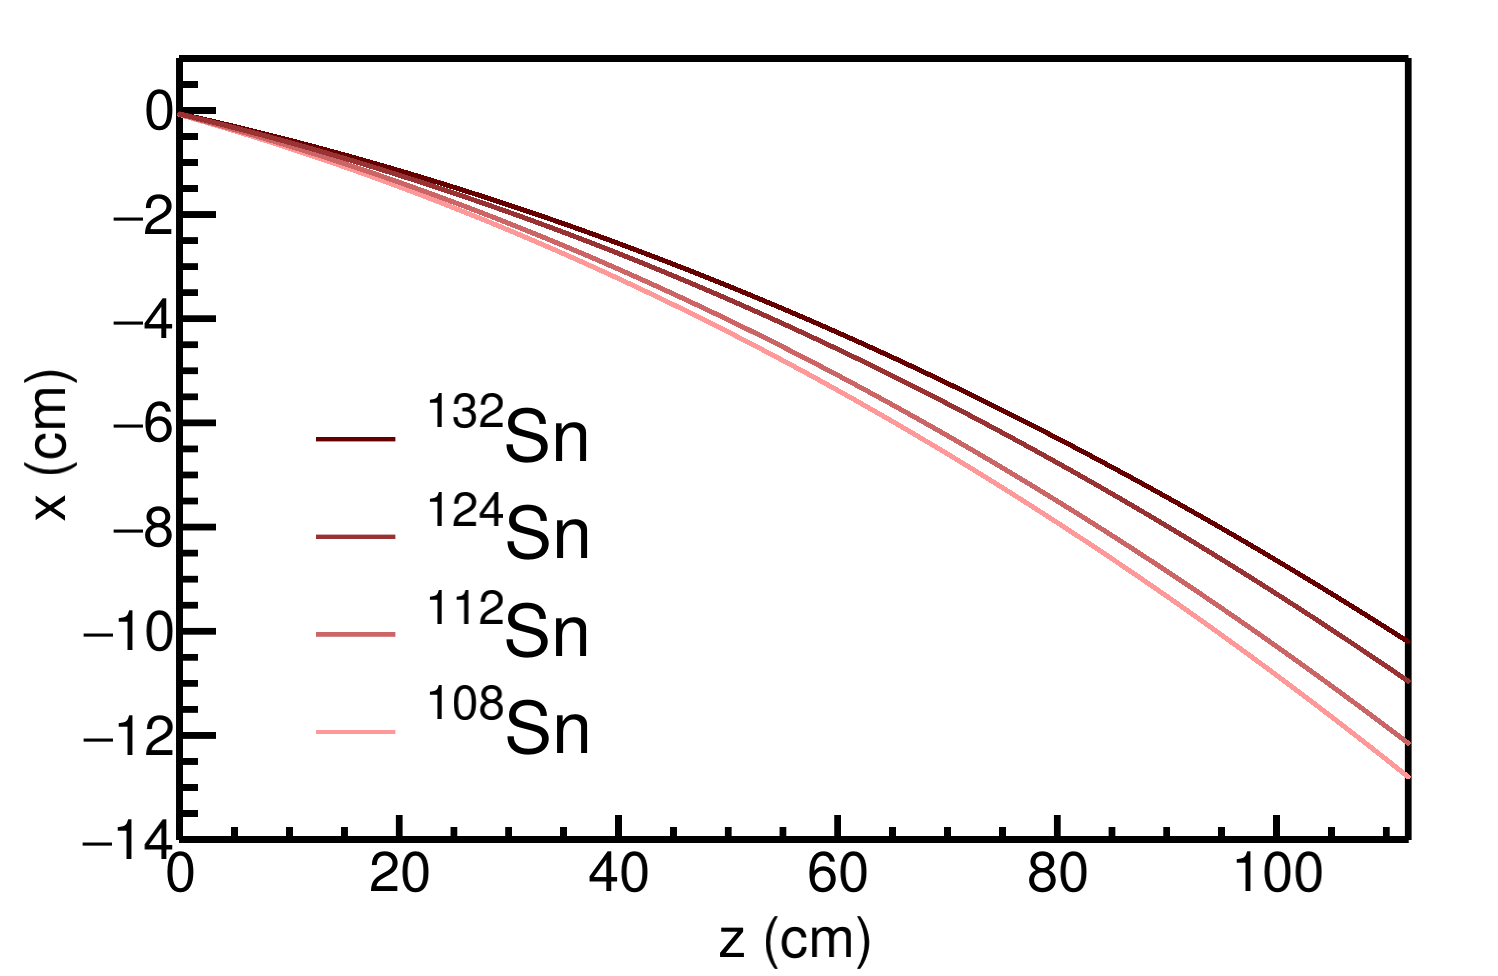
\includegraphics[width=\linewidth]{beampath.png}
\caption{Beam path of the experiments}
\label{fig:beampaths}
\end{figure}
 
 
 The beam is positioned about \SI{25}{\centi\metre} below the anode plane and \SI{29.6}{\centi\metre} above the cathode in the TPC. It takes electrons approximately 5\si{\micro\sec} to drift to the anode plane where as it takes the ions \num{5e4}\si{\micro\sec} to drift to the cathode. The beam rate in the experiment was approximately \SI{10}{\kilo\hertz}, which has an average occurrence of 1 beam every \SI{100}{\micro\sec}. This is  much shorter than the time it takes for the ions to terminate on the cathode plane, resulting in a build up of positive ions. Figure~\ref{fig:spacechg_cartoon} gives an idea of the shape of the sheet of space charge carved out by the beam path. The ions from each beam create a line charge which drifts towards the cathode with a constant velocity. The average distance between sequential ion paths is about \SI{25}{\micro\metre} apart, therefore we expect the average number of beam paths that make up the sheet charge is around \num{1440} tracks. Since the number of tracks in the sheet charge is large, and inter beam spacing is very small, this allows us to approximate the sheet charge as an uniform sheet charge density. 
 
 The secondary beams entering the TPC are also composed of many species of particles distributed in a finite range around the target beam as will be discussed in Section~\ref{sec:beam}. Let us assume a beam of ${}^{132}$Sn where the energy loss in P10 gas, at 270 AMeV, is \SI{11.2}{\kilo\electronvolt\per\centi\metre}. From the total number of beams above, and the beam path length of \SI{135}{\centi\metre}, the estimated charge density would be on the order of \SI{3e-8}{\coulomb\per\metre\squared}. 
 

The electric potential can be calculated by solving Poisson's equation, 

\begin{equation}
\nabla^2 \phi = \rho,
\end{equation}

 where $\phi$ is the electric potential and $\rho$ is the free charge. The numerical solution is provided by the Jacobi method \cite{poisson} provided all 6 sides have defined Dirchlet boundary conditions for the potentials. We neglect the wire plane region since the drift details are not important for the space charge effects we are discussing here. The pad plane and cathode are trivial, where the side walls of the field cage are given linearly varying potentials on the surface such that the electric field is the same strength as the real TPC with no space charge present. Once the electric potential is solved, the electric field is simply the gradient of the potential  $\vec{E}= -\nabla \phi$. 
 
It has been shown before that the amount of space charge present in the chamber is related to observables such as the distance-of-closest-approach (dOCA) of each track to the vertex point \cite{starSC}. In the presence of no space charge, the dOCA distribution of each track would be a centered around the true vertex location. Since the tracks are distorted by the space charge, which affects different regions of the TPC differently, a bias is introduced to the measured vertex location and widens the distribution to vertex of each track.  

An example of the distortion map in the TPC is shown in Fig.~\ref{fig:sc_shift} where left-going tracks shown in blue, and right-going tracks shown in green. The vectors show the direction of distortion, and their magnitude have been magnified by 10 times to show the detail. The dashed lines show the shifted track due to the space charge where left and right-going tracks are affected differently. Right-going tracks tend to higher momentum values and the left-going tracks going to lower momentum values, for positively charged particles.  
 

\begin{figure}[!htb]
\centering
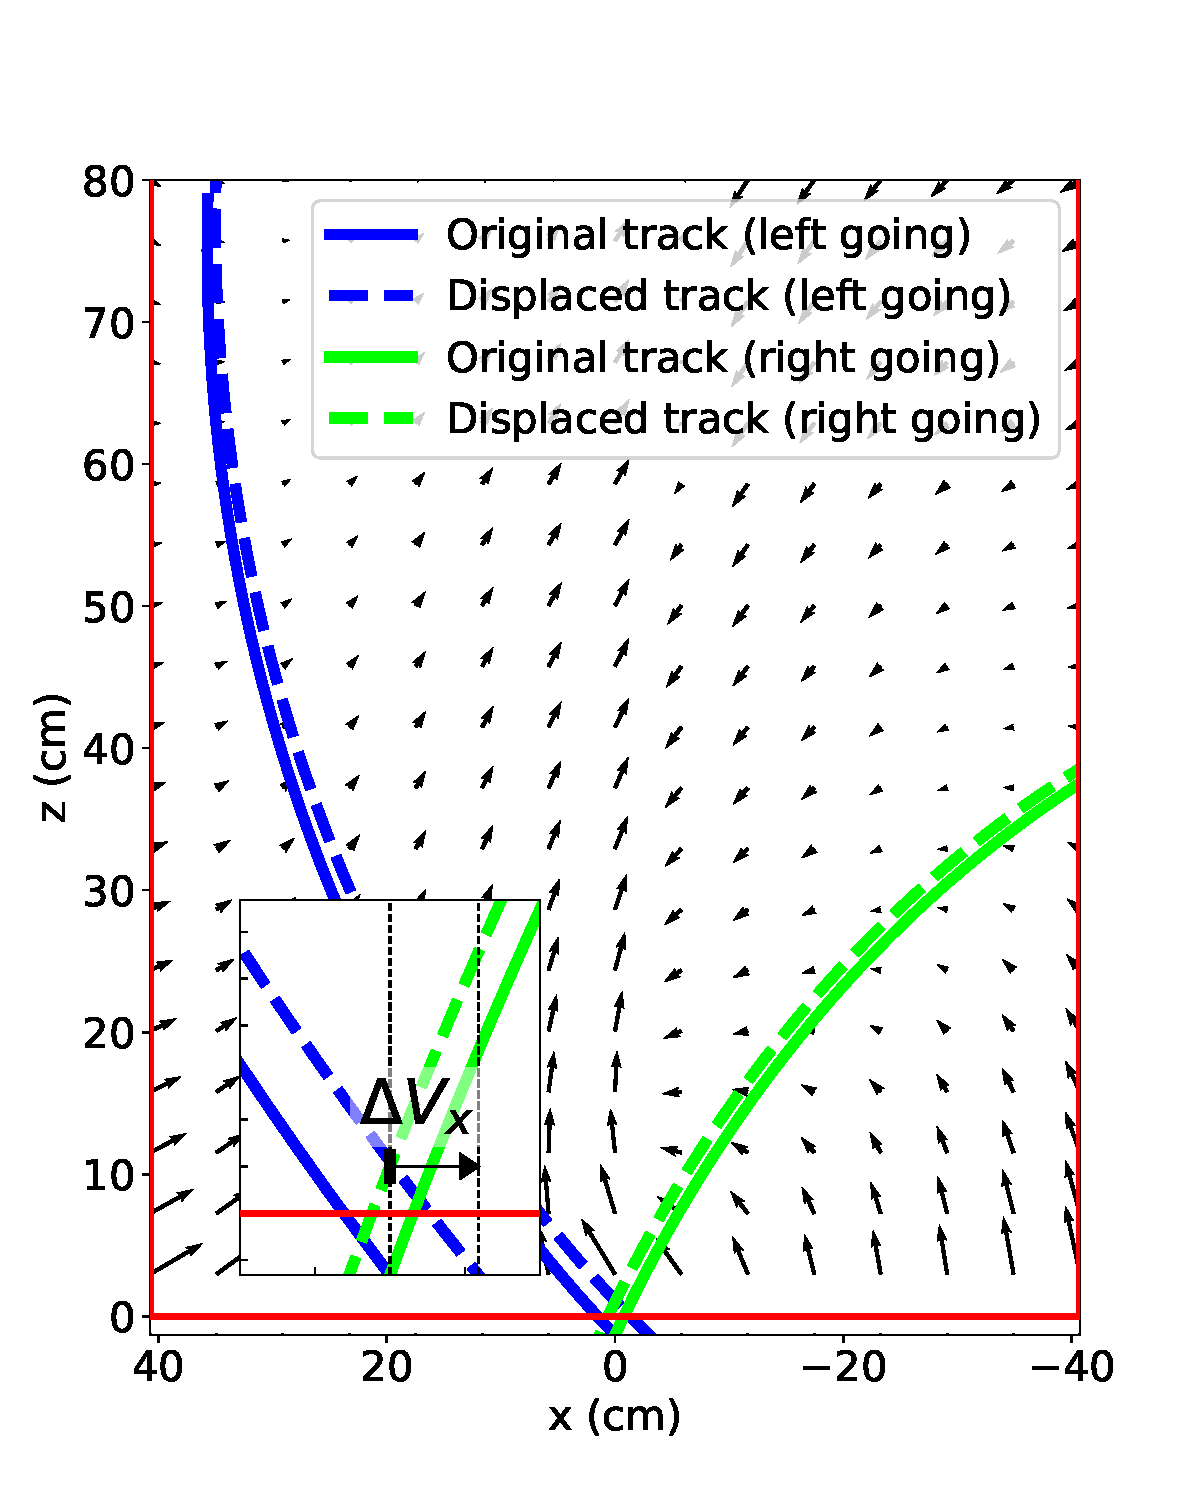
\includegraphics[scale=.5]{Effect_SC.pdf}
\caption{Example of the map of the electron shift. The effect is also shown on left-going (blue) and right-going (green) tracks. The original tracks are shown in the solid line and the shifted track in the dotted line.}
\label{fig:sc_shift}
\end{figure}

The inset figure of Fig.~\ref{fig:sc_shift} shows the effects of the space charge have on the x-component of the dOCA to the vertex for the displaced left-going track given by $\Delta\mathrm{V}_\mathrm{x}$, with the opposite direction for right-going tracks. Figure~\ref{fig:VLR} shows the amount of distortion caused by the space charge effect as a new observable $\Delta\mathrm{V}_\mathrm{LR} = \Delta\mathrm{V}_\mathrm{x}^L - \Delta\mathrm{V}_\mathrm{x}^R$ , where  $V_x^L$ and $V_x^R$ are the most probable value of the dOCA distribution for left and right-going tracks respectively. 

\begin{figure}[!htb]
\centering
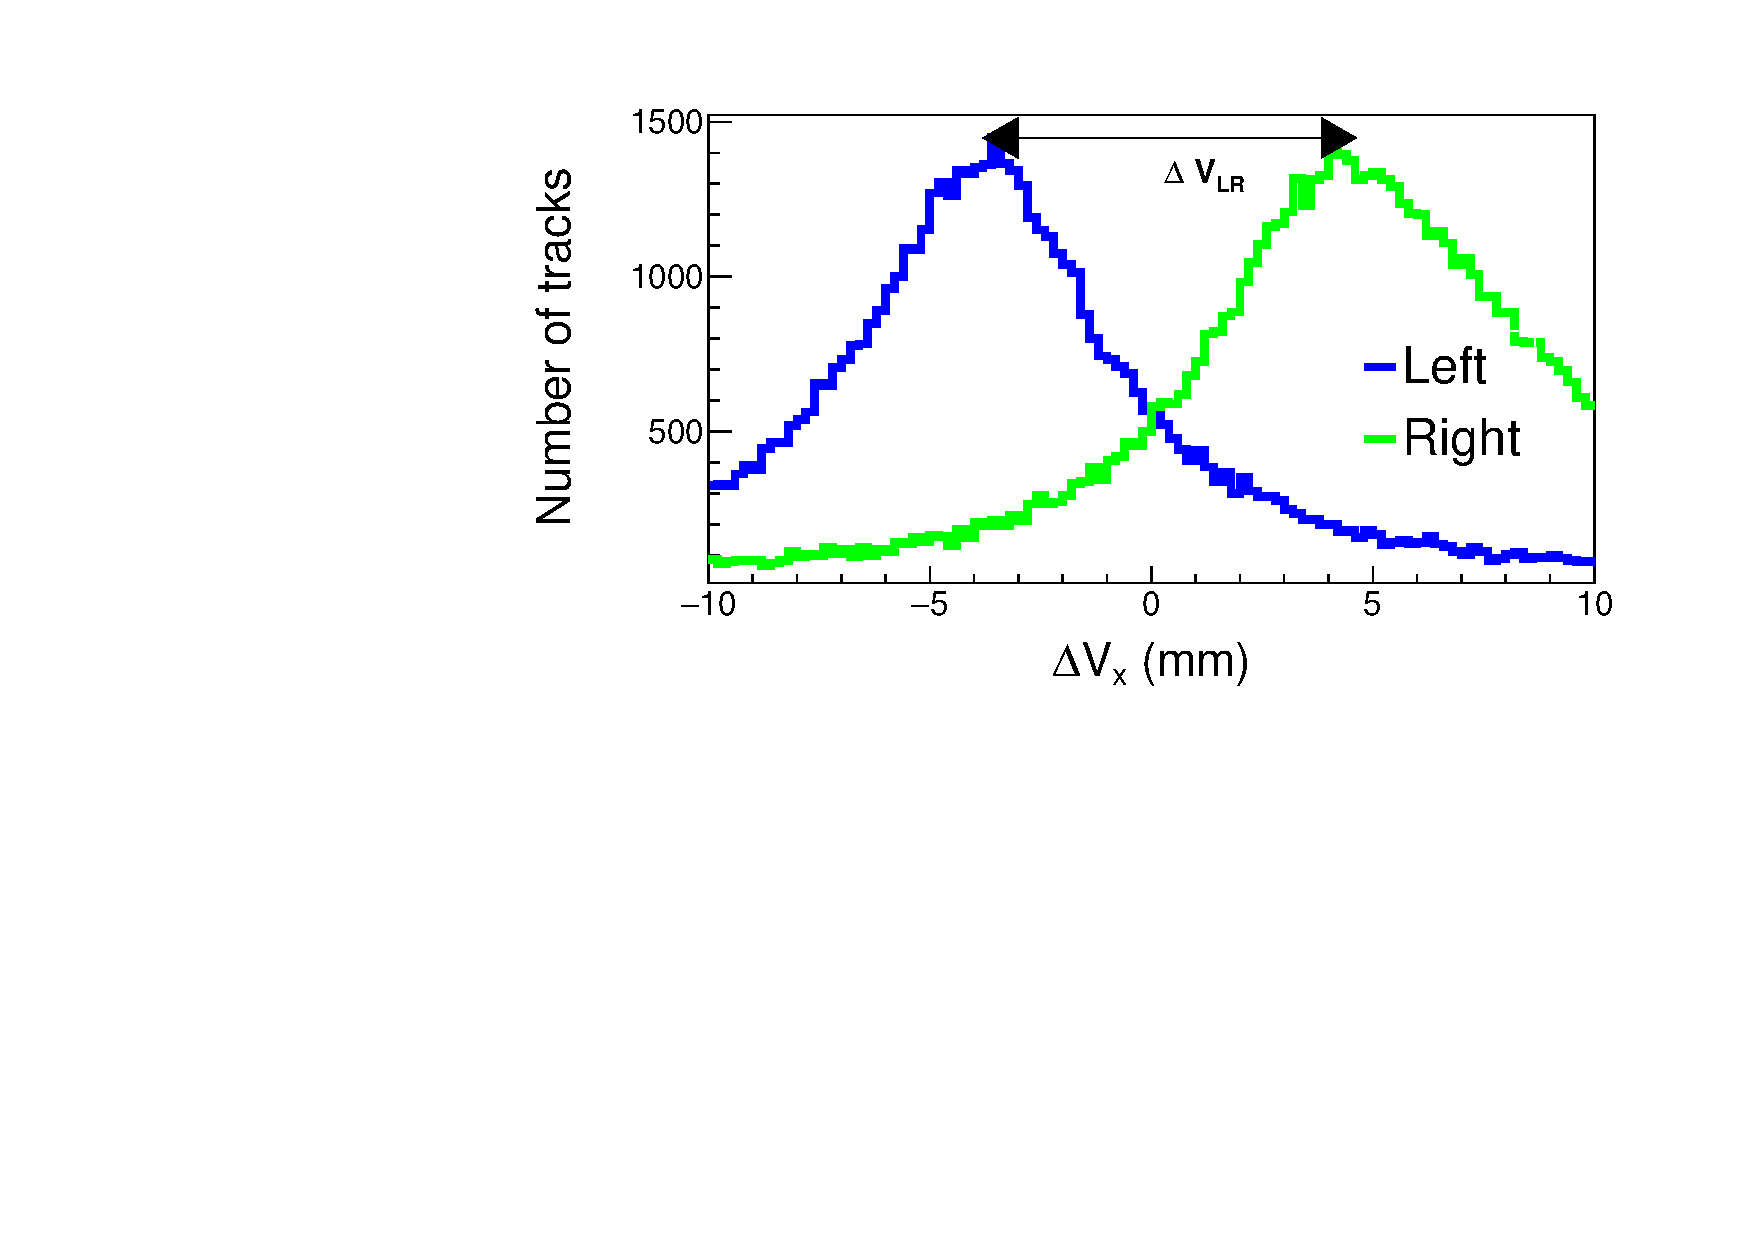
\includegraphics[scale=.5]{DVTP_raw.pdf}
\caption{$\Delta\mathrm{V}_\mathrm{x}$ distribution for left-going and right-going tracks. }
\label{fig:VLR}
\end{figure}



\begin{figure}[!htb]
\centering
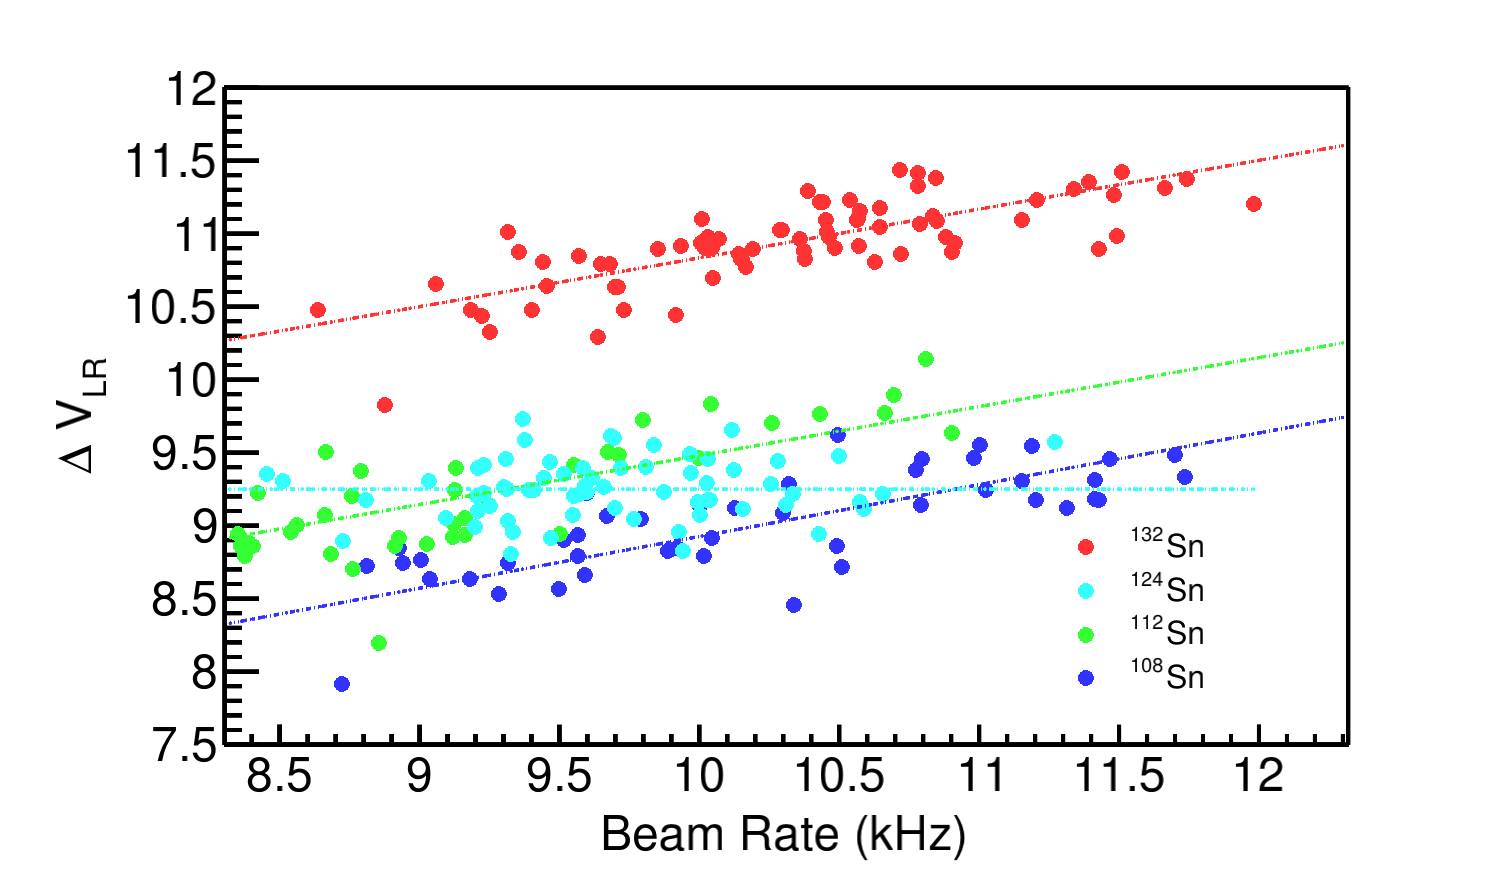
\includegraphics[width=\linewidth]{VLR_beamrate.png}
\caption{ $\Delta V_{LR}$ versus the beam rate for all systems with the fitted function.}
\label{fig:VLR_br}
\end{figure}



\begin{figure}[!htb]
\centering
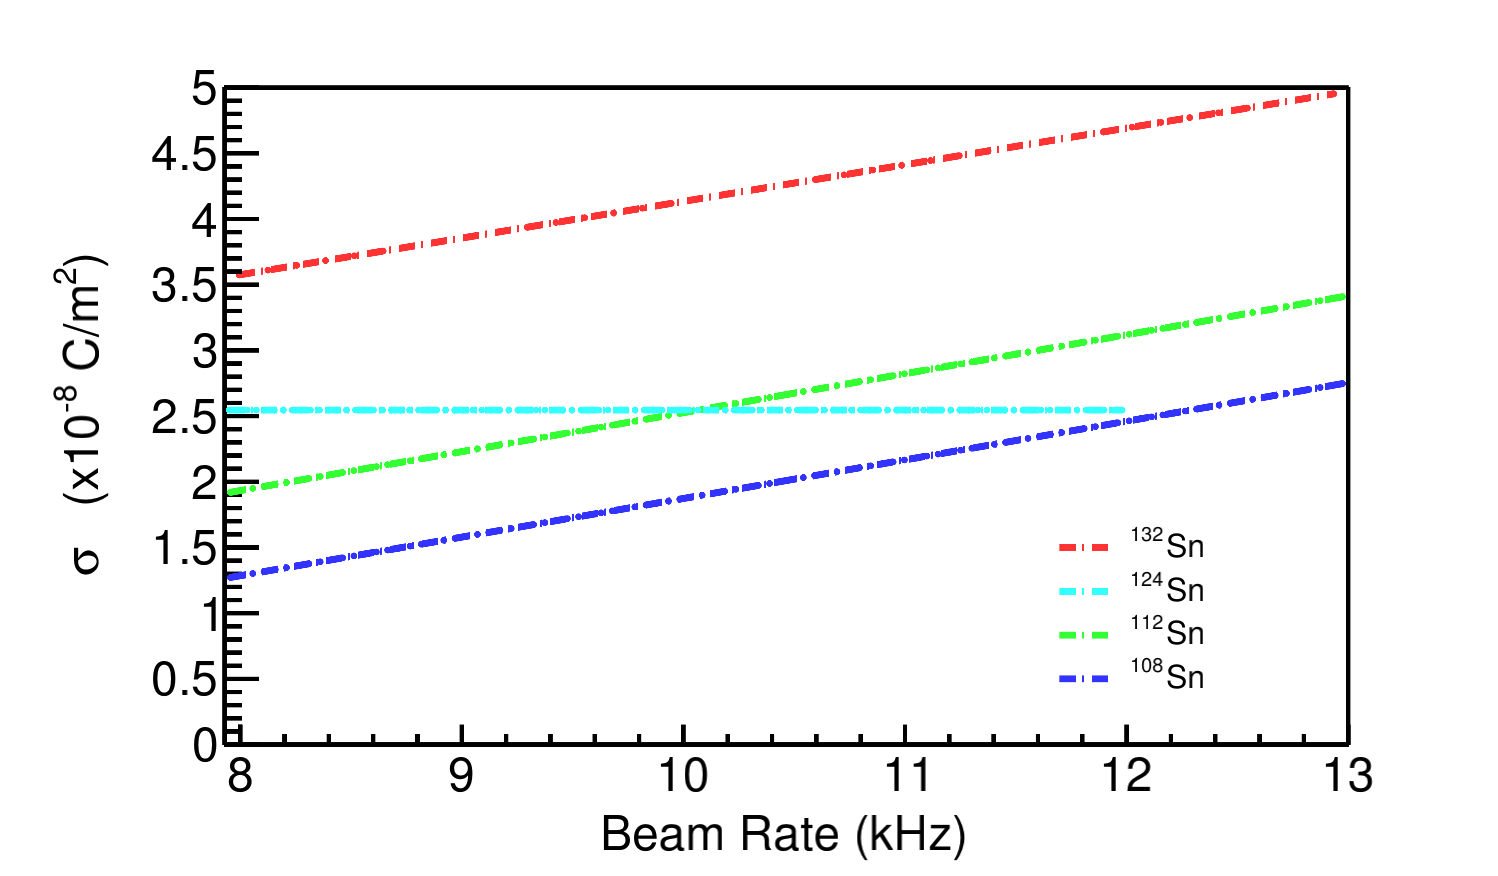
\includegraphics[width=\linewidth]{sc_beamrate.png}
\caption{Space charge fit function versus the beam rate for all systems. These are the assumed functions we use for interpolating the space charge value from the beam rate.}
\label{fig:spacechg_br_all}
\end{figure}

The average beam rate was recorded in each experimental run and slightly varied from run to run, due to beam production variations. The amount of space charge present in the field cage is directly proportional to the beam rate; therefore $\Delta\mathrm{V}_\mathrm{LR}$ is also proportional to the beam rate as shown in Fig.~\ref{fig:VLR_br}. The only parameter in the space charge correction algorithm is the surface charge density $\sigma_{\mathrm{SC}}$. Varying $\sigma_{\mathrm{SC}}$ for a wide range of values the $\Delta\mathrm{V}_\mathrm{LR}$ observable is measured and plotted in the left panel of Fig.~\ref{fig:spacechg_relation}. The surface charge density which gives $\Delta\mathrm{V}_\mathrm{LR} = 0$ is taken to be the estimate for the average amount of space charge present. 

This is done for several runs which vary in beam intensity though the solution for the estimated space charge value will be different. Since the surface charge density is proportional to the beam rate, a linear fit gives good agreement for interpolating the surface charge values as a function of beam rate. Figure~\ref{fig:spacechg_relation} shows the relation of the dependence of the space charge as a function of beam rate for the ${}^{132}$Sn system.

\begin{figure}[!htb]
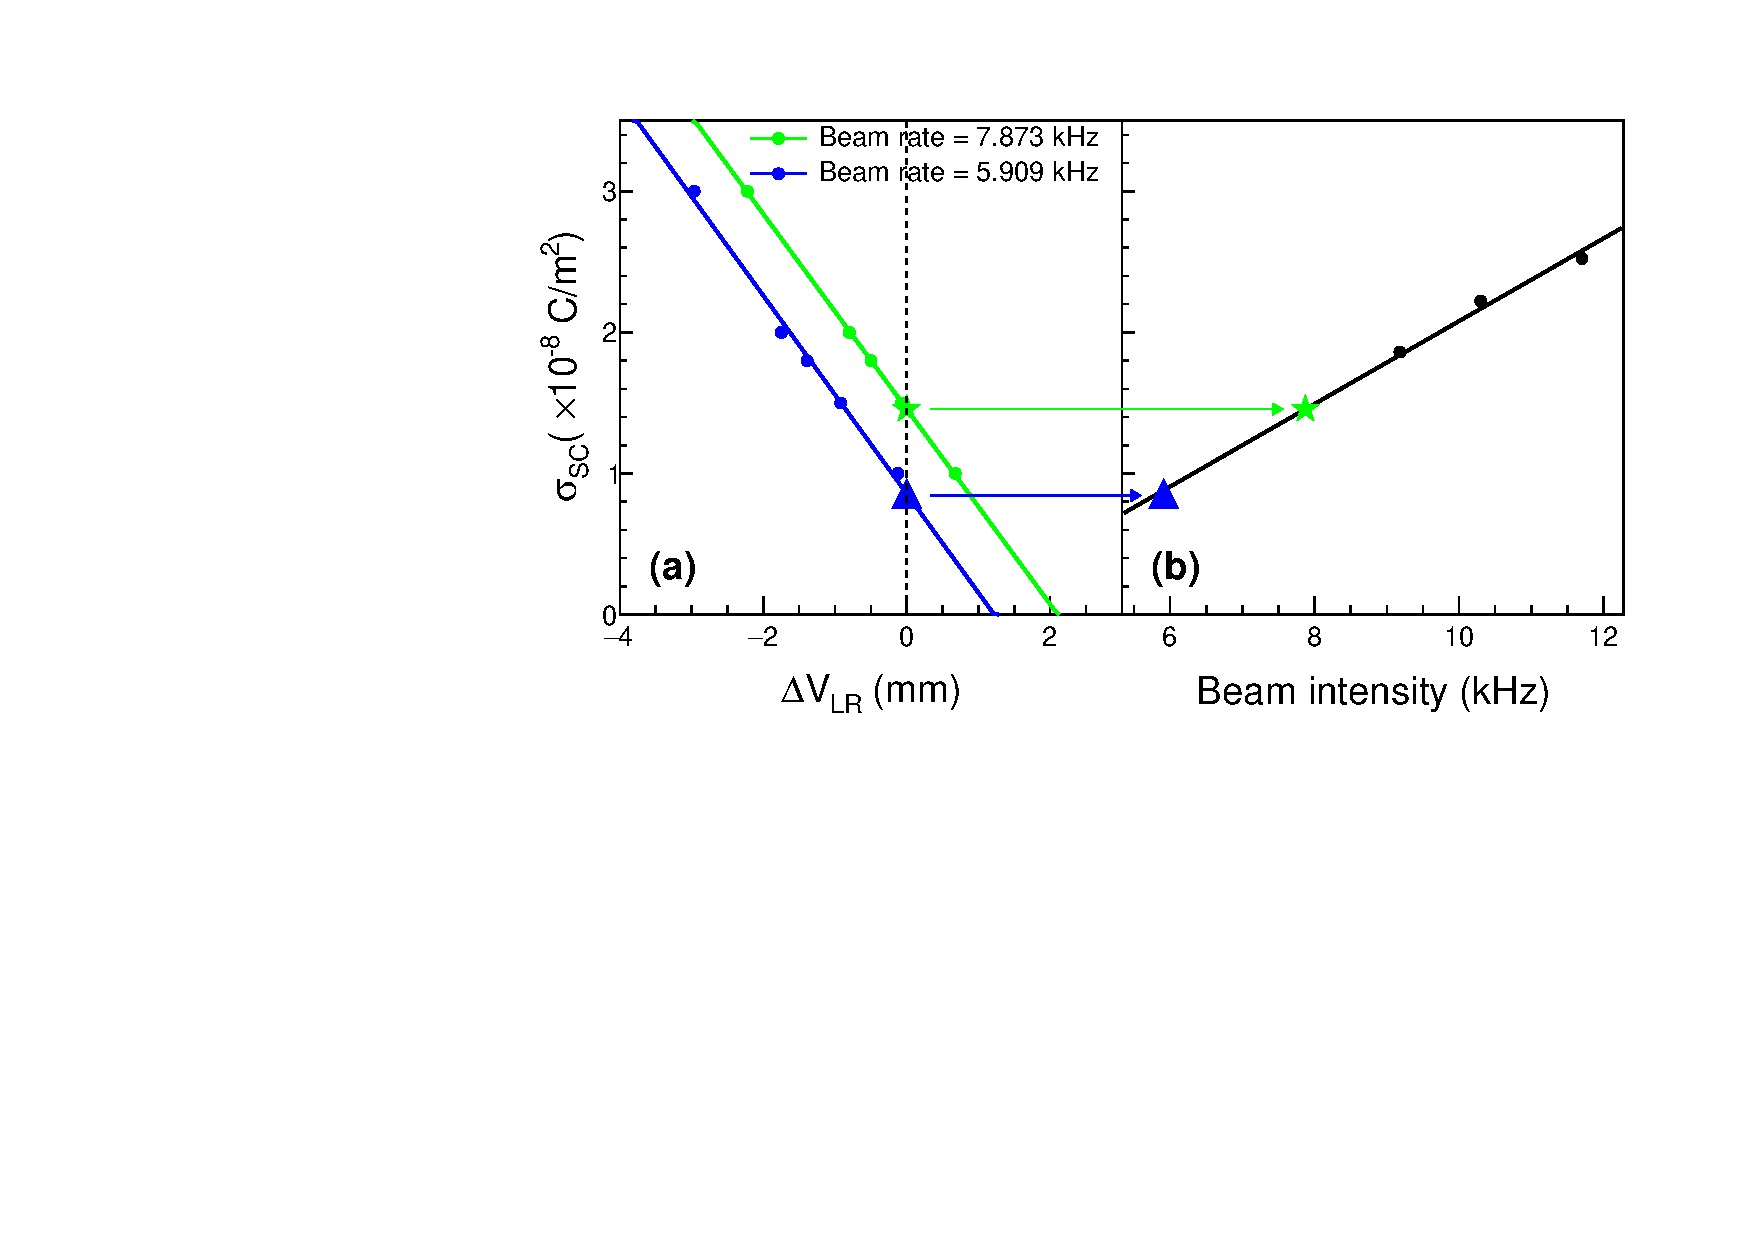
\includegraphics[width=\linewidth]{SC_Relation.pdf}
\caption{Space charge relation}
\label{fig:spacechg_relation}
\end{figure}


Following this algorithm the space charge is estimate for each run and system. Figure~\ref{fig:scDensity} shows the summary of the extracted space charge values for each secondary beam. The linear fits relating the space charge density to the beam rate for each system is shown in Fig.~\ref{fig:spacechg_br_all} where the space charge value is inferred from the measured beam rate. Notice that in the $\tin{112}{124}$ system a constant value of was assumed since the beam rate did not span a large enough range to warrant a more detailed analysis. 

To reduce the need to compute a new electric field for each space charge value, notice that $\vec{E}\propto \rho$, we can therefore solve the electric field for a certain reference charge value $\rho_o$, and scale the solution for any other free charge $\rho$ by the ratio $\rho/\rho_o$. The full magnetic field map is provided by the SAMURAI collaboration \cite{magnet}. The velocity field map is calculated following Eq.~\ref{eq:elecdrift}. The electron drift through this velocity map is propagated by using a time stepped $\mathrm{4}^{\mathrm{th}}$-Order Runge-Kutta integration from a certain starting point.
  
 The correction map is calculated by starting from the anode y-position and the measured position on the pad-plane (x,z), and stepping backward in time in the Runge-Kutta integration, through the velocity field map until the electron reaches the measured y-position. This is done over a 3-dimensional grid where points in between are interpolated by a trilinear interpolation. The measured clusters value (x,y,z) position is input into the correction map which outputs the interpolated correction values $dx$ and $dz$ which correspond to that cluster. The cluster position is then shifted to new positions $x\textprime = x + dx$ and $z\textprime = z + dz$.
 

%What is the best figure to put in? VLR vs Charge density? 
%estimate of the error of VLR and how it corresponds to charge density

\begin{figure}[!htb]
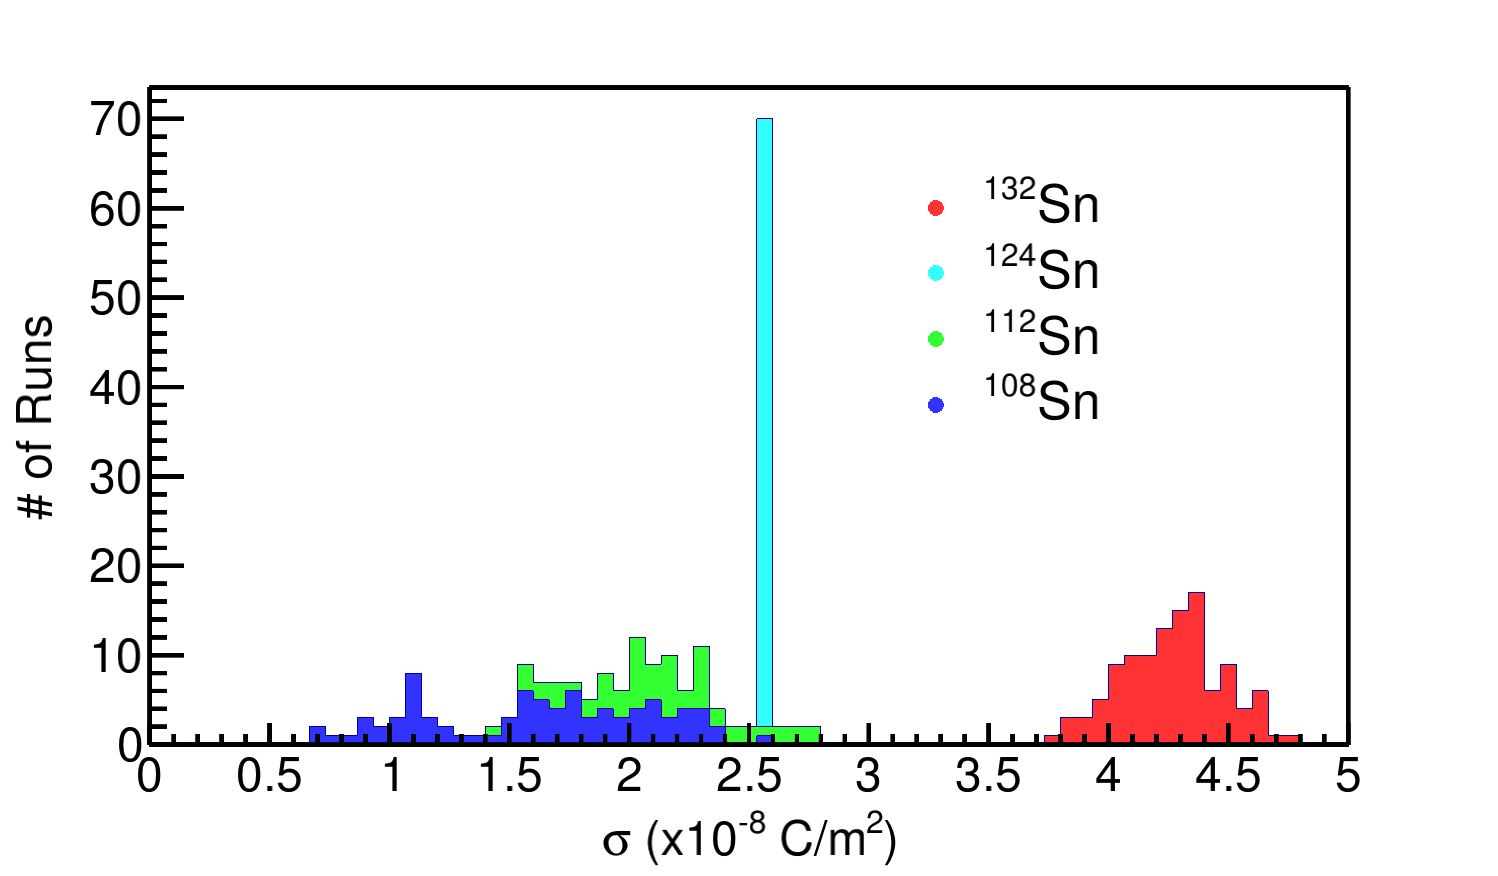
\includegraphics[width=\linewidth]{spaceChgDensity.png}
\caption{Distribution of estimated space charge densities for each beam type.}
\label{fig:scDensity}
\end{figure}



\begin{figure}[!htb]
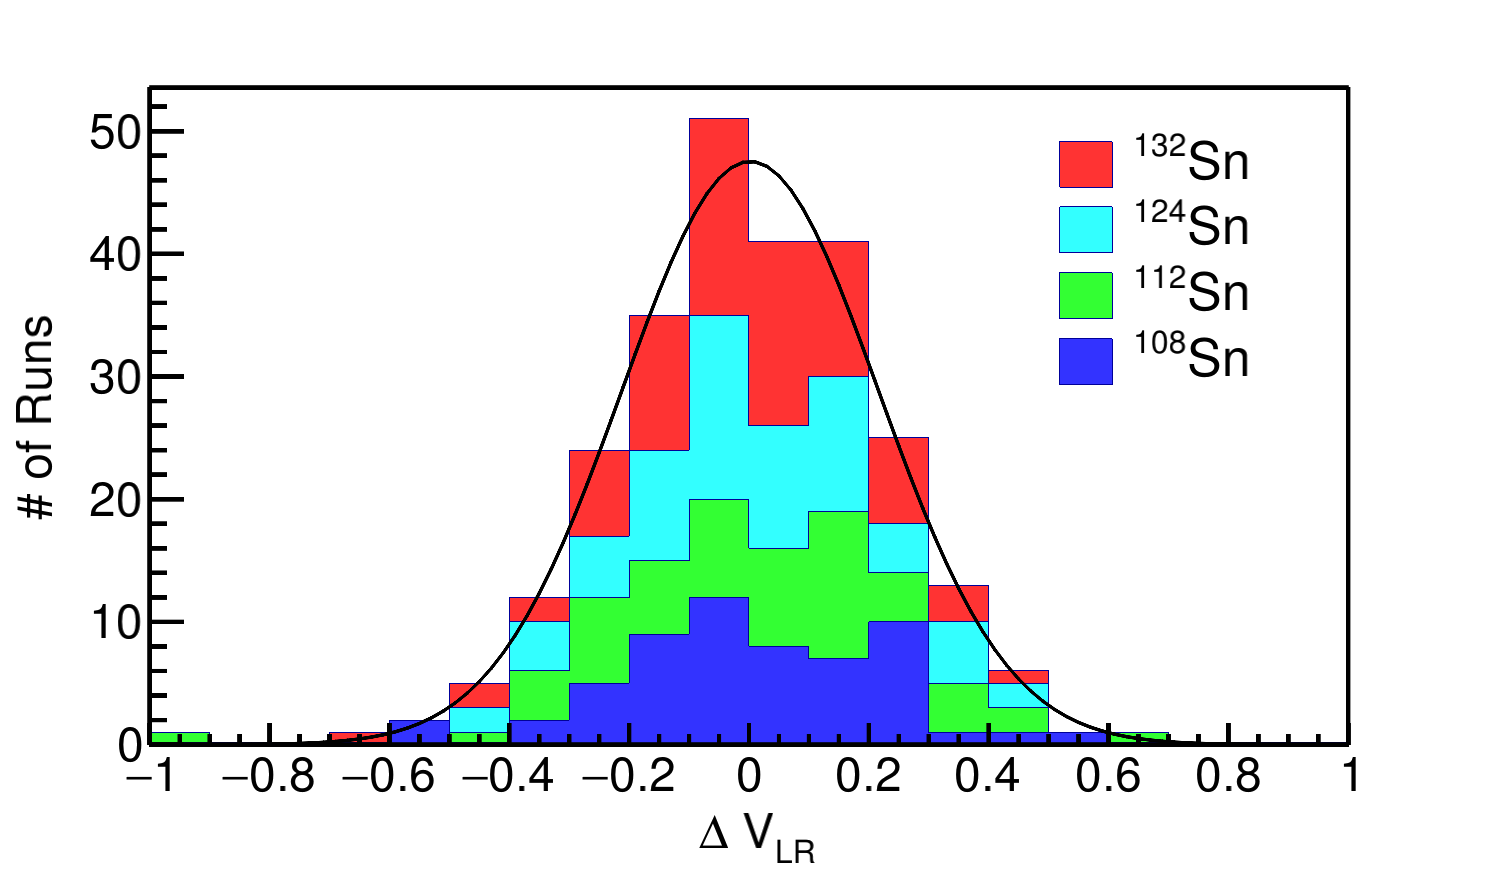
\includegraphics[width=\linewidth]{VLRresidual.png}
\caption{Residuals in the fitted line of $\Delta V_{LR}$ observable for all systems.}
\label{fig:vlrResidual}
\end{figure}

Adding the BDC vertex greatly improves the momentum resolution of the track fitting, but there is a systematic shift when as compared with the momentum value without using a vertex as an extra constraint. Since the space charge affects right-going and left-going tracks differently making right-going tracks differently than left-going tracks, it appears they no longer originate from the BDC which is not affected by the space charge. For tracks at polar angles of $\theta_{Lab} < \ang{40}$, the disagreement between momentum values with and without the BDC are much less because the projection of the track does not disagree as much with the BDC point as shown in Fig.~\ref{fig:mom_S_before}. Figure~\ref{fig:mom_L_before} shows the momentum value of tracks going at polar angles of $\theta > 40 \deg$ which are more sensitive to small changes in the BDC when including it as an extra constraining point. After correcting for the space charge and adding the BDC point, the reconstructed momentum value agrees with or without the BDC included for both  $\theta_{Lab} < \ang{40}$ or $\theta_{Lab} > \ang{40}$, as seen in Fig.~\ref{fig:mom_S_after} and Fig.~\ref{fig:mom_L_after} respectively. 


\begin{figure}[!htb]
    \centering
    \begin{subfigure}[t]{0.45\textwidth}
        \centering
        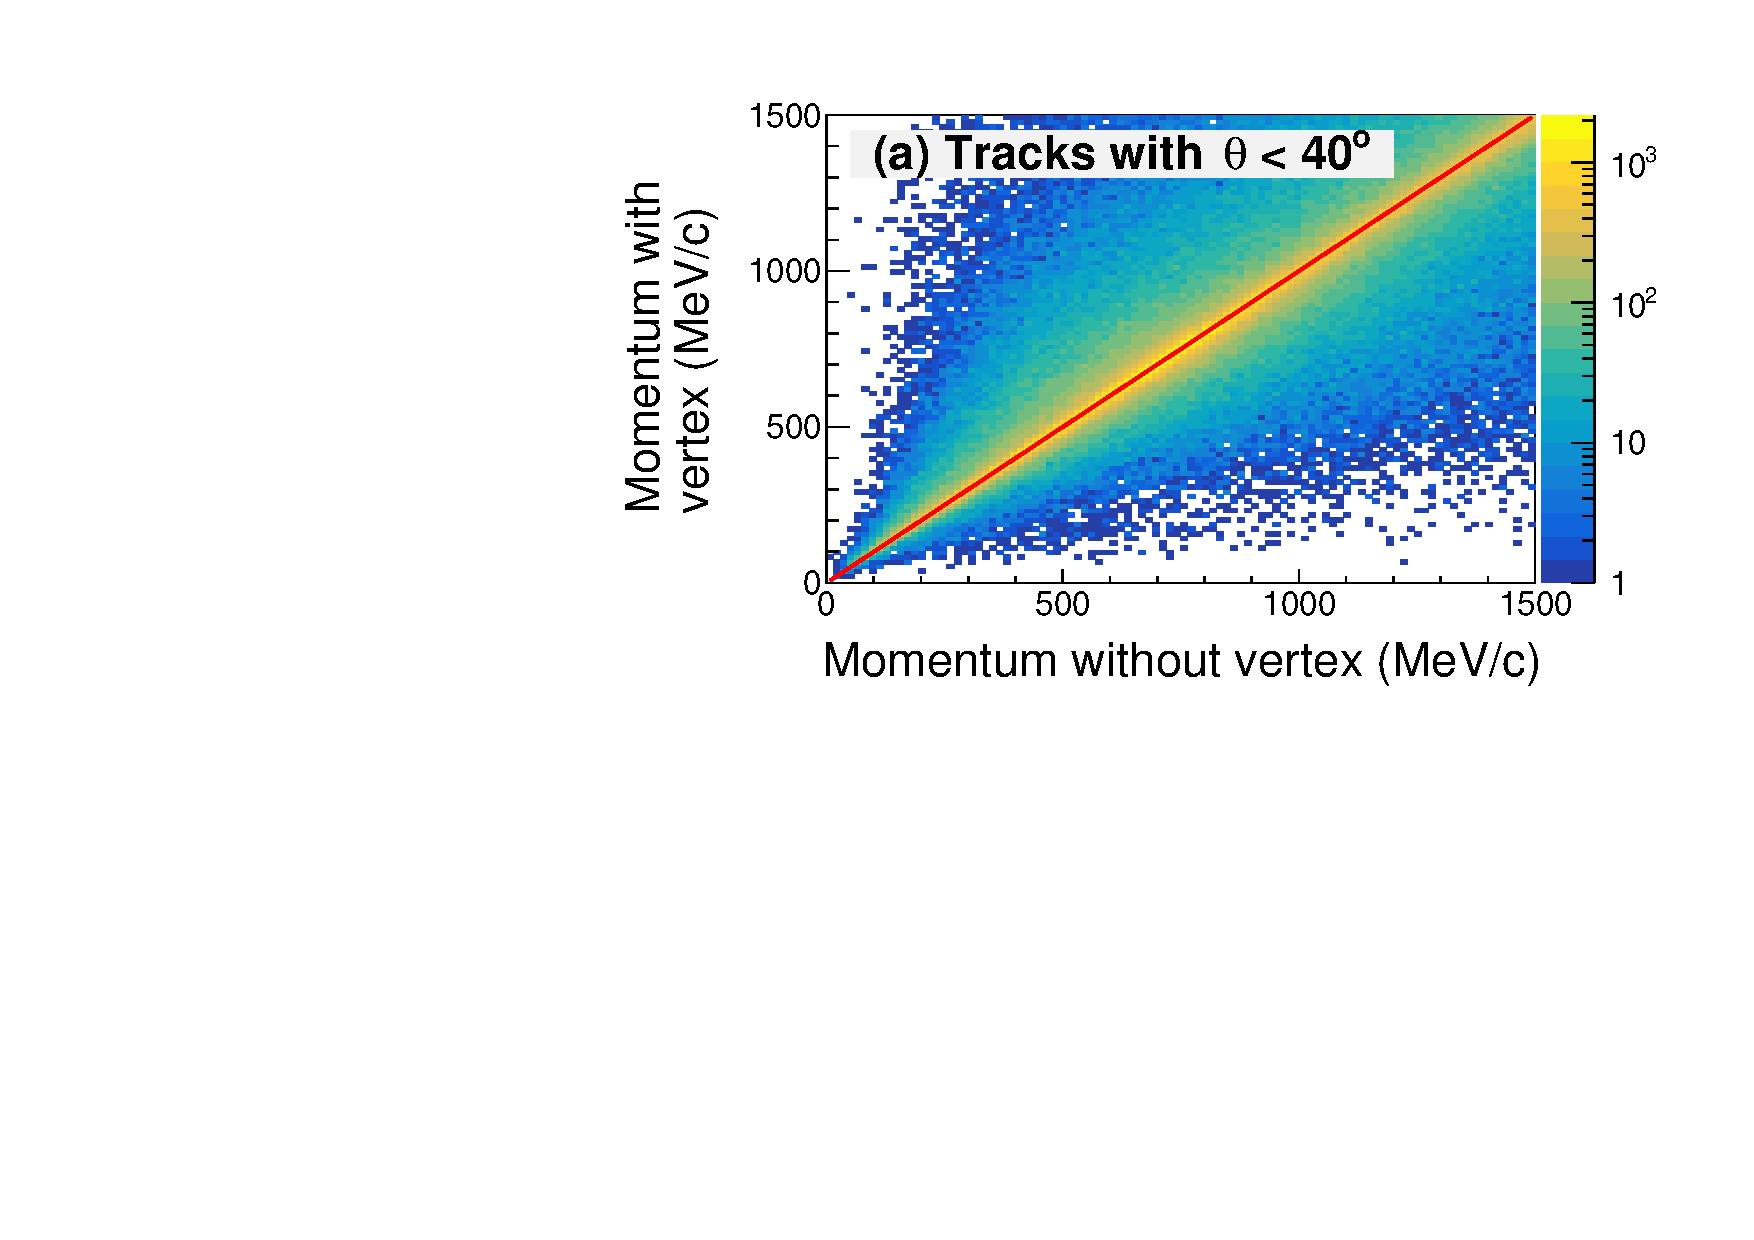
\includegraphics[width=\linewidth]{BDC_P_small_angle.pdf} 
        \caption{Compare the momentum before and after including the BDC vertex for tracks with $\theta_{Lab} < \ang{40}$, before the space charge correciton.} \label{fig:mom_S_before}
    \end{subfigure}
    \hfill
    \begin{subfigure}[t]{0.45\textwidth}
        \centering
        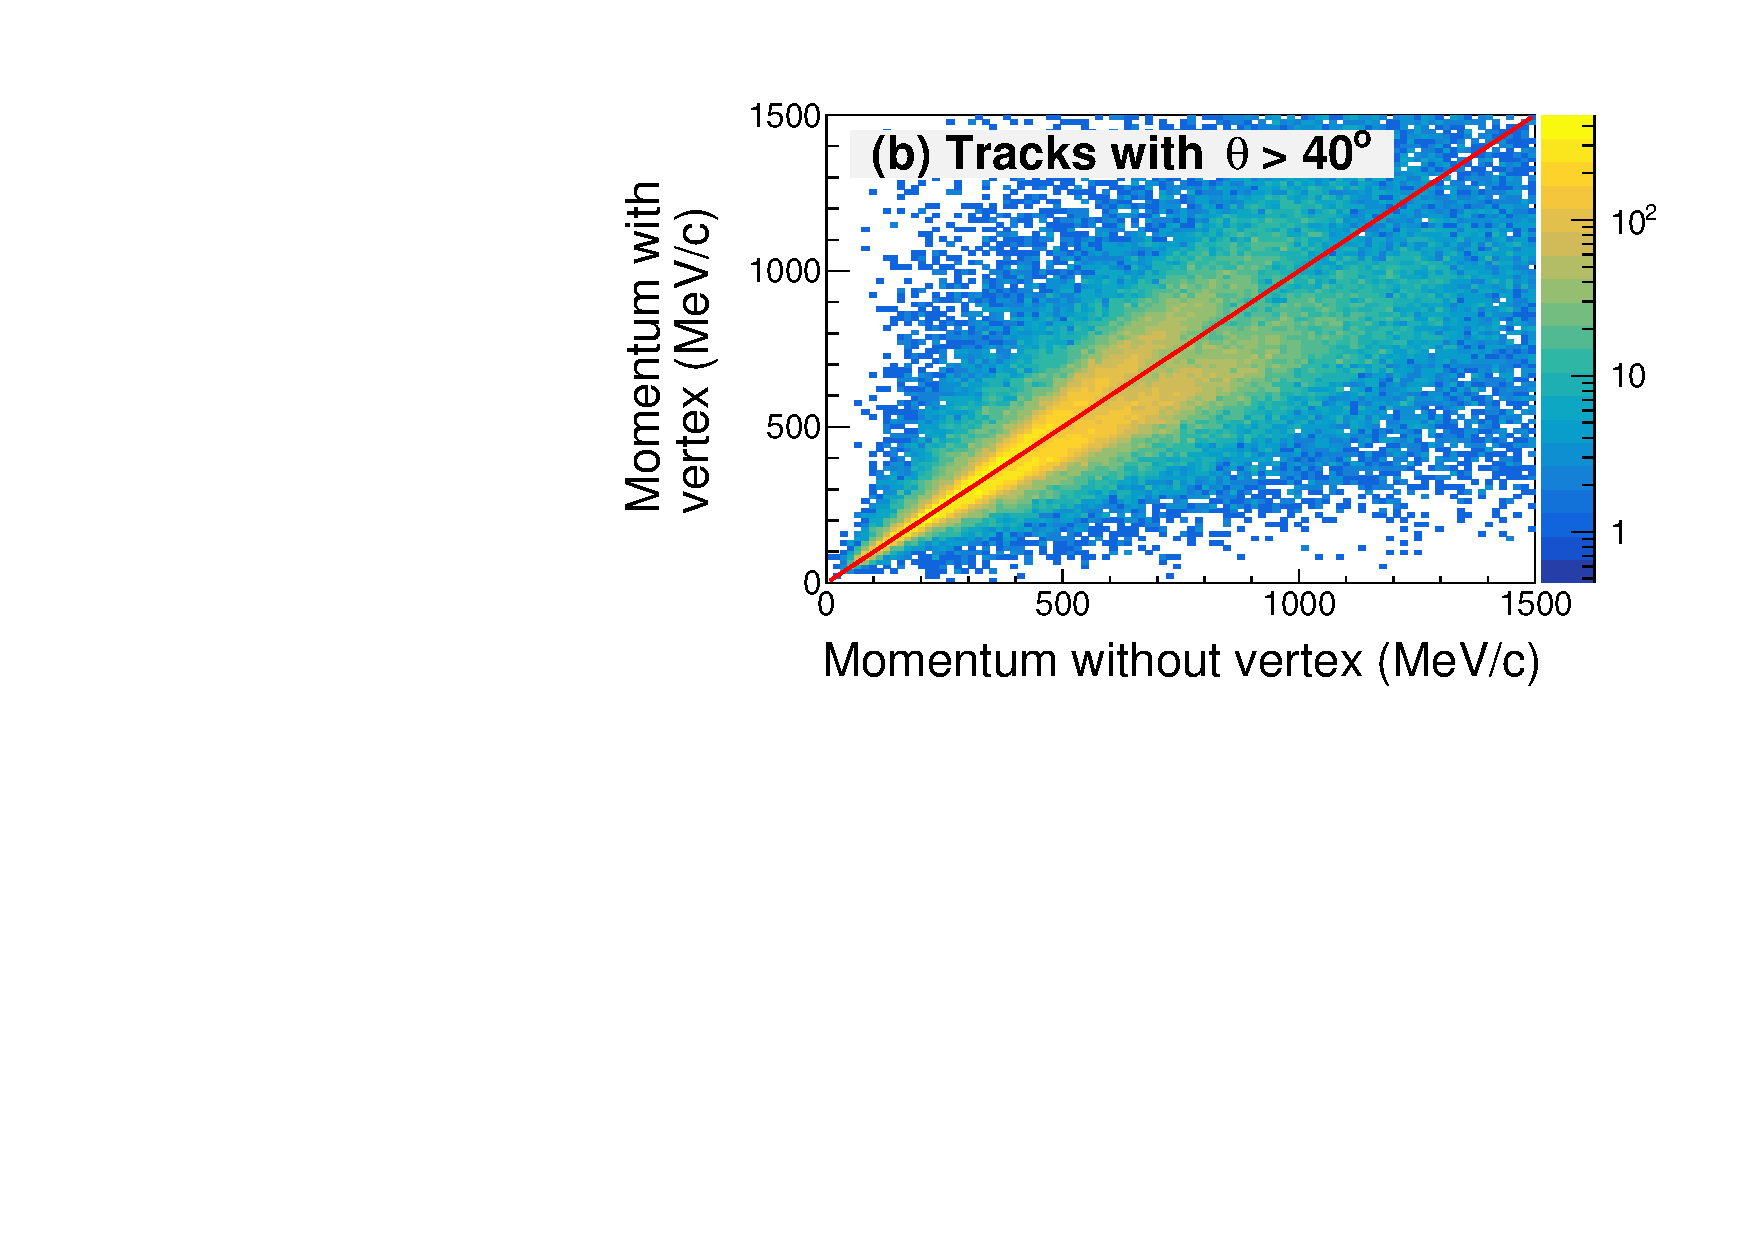
\includegraphics[width=\linewidth]{BDC_P_large_angle.pdf} 
        \caption{Comparison of the momentum before and after including the BDC vertex for tracks with $\theta_{Lab} > \ang{40}$, before the space charge correction.} \label{fig:mom_L_before}
    \end{subfigure}
    
    \begin{subfigure}[t]{0.45\textwidth}
        \centering
        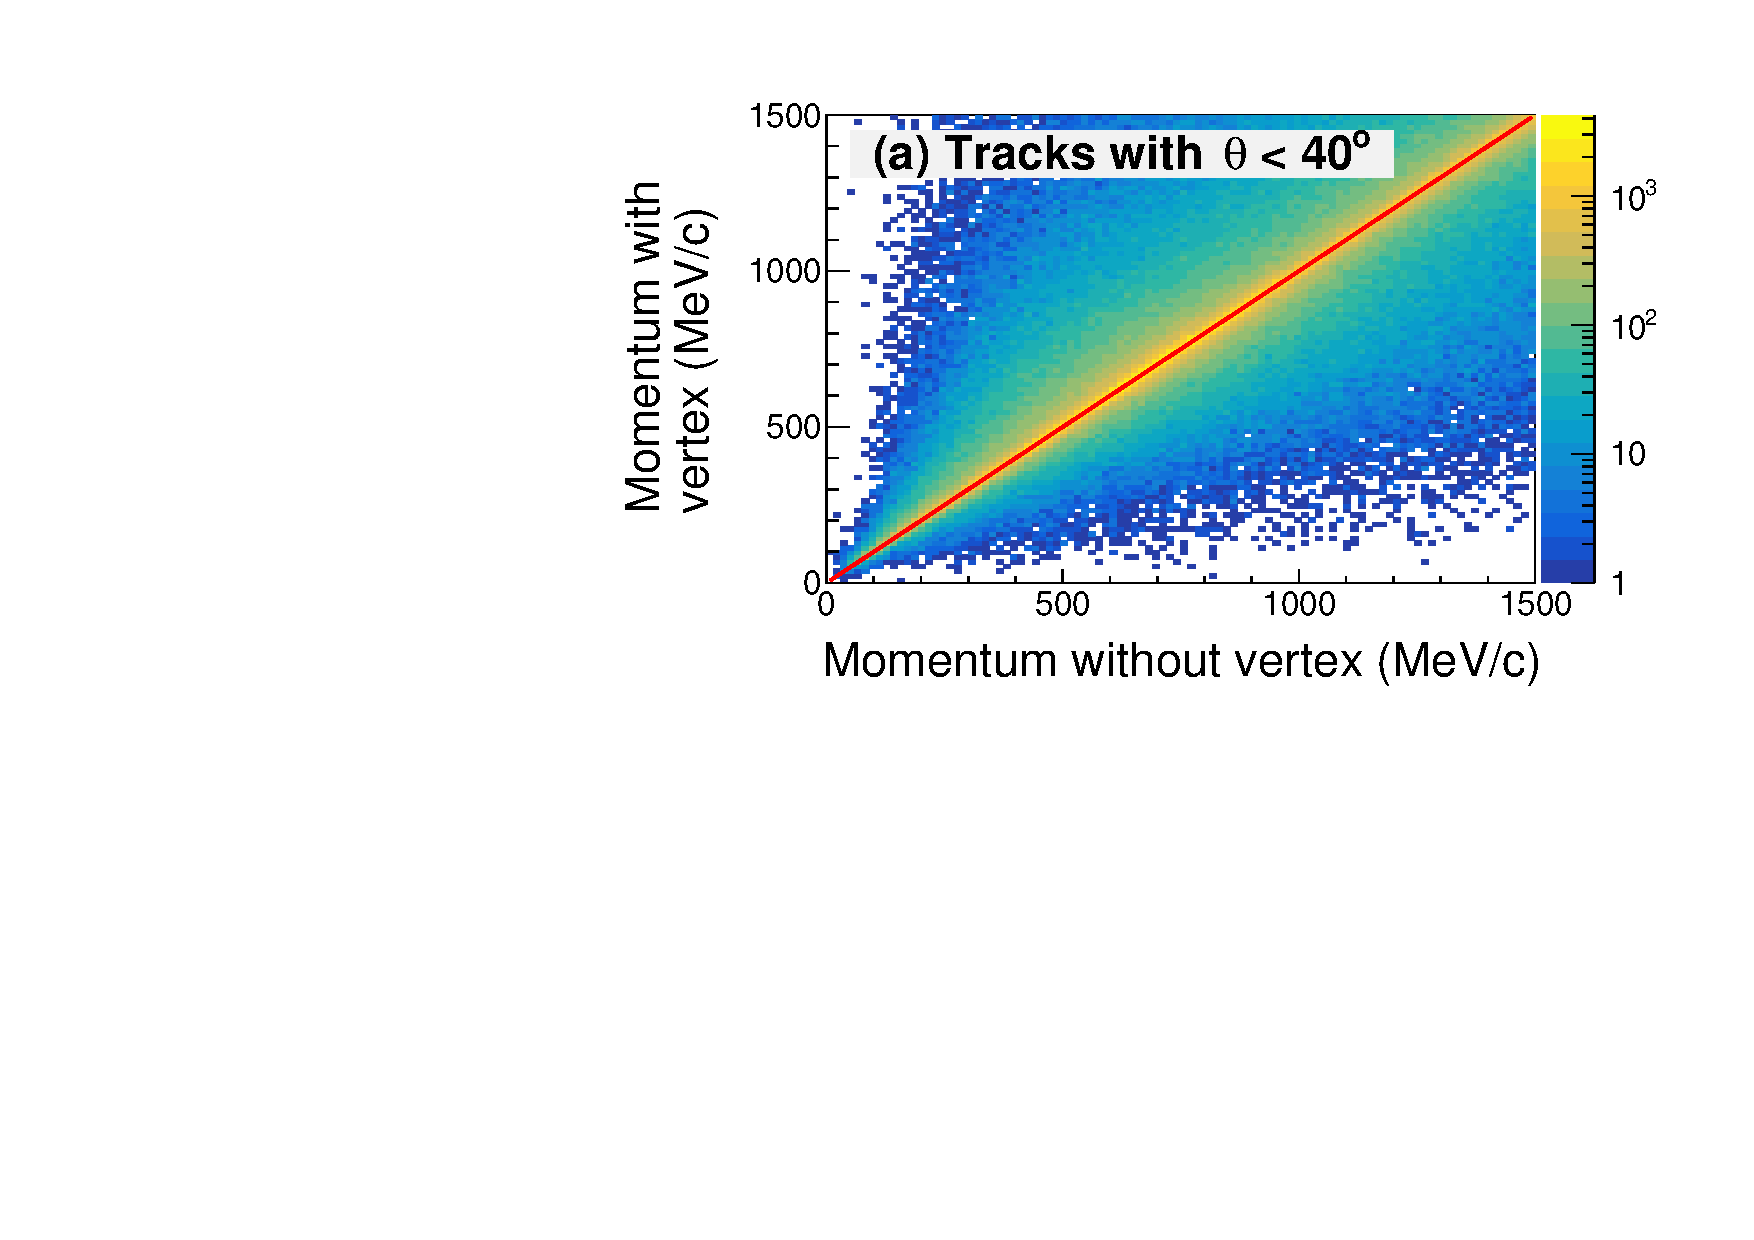
\includegraphics[width=\linewidth]{BDC_P_aftercor_small_angle.pdf} 
        \caption{Compare the momentum before and after including the BDC vertex for tracks with $\theta_{Lab} < \ang{40}$, after the space charge correction. } \label{fig:mom_S_after}
    \end{subfigure}
    \hfill
    \begin{subfigure}[t]{0.45\textwidth}
        \centering
        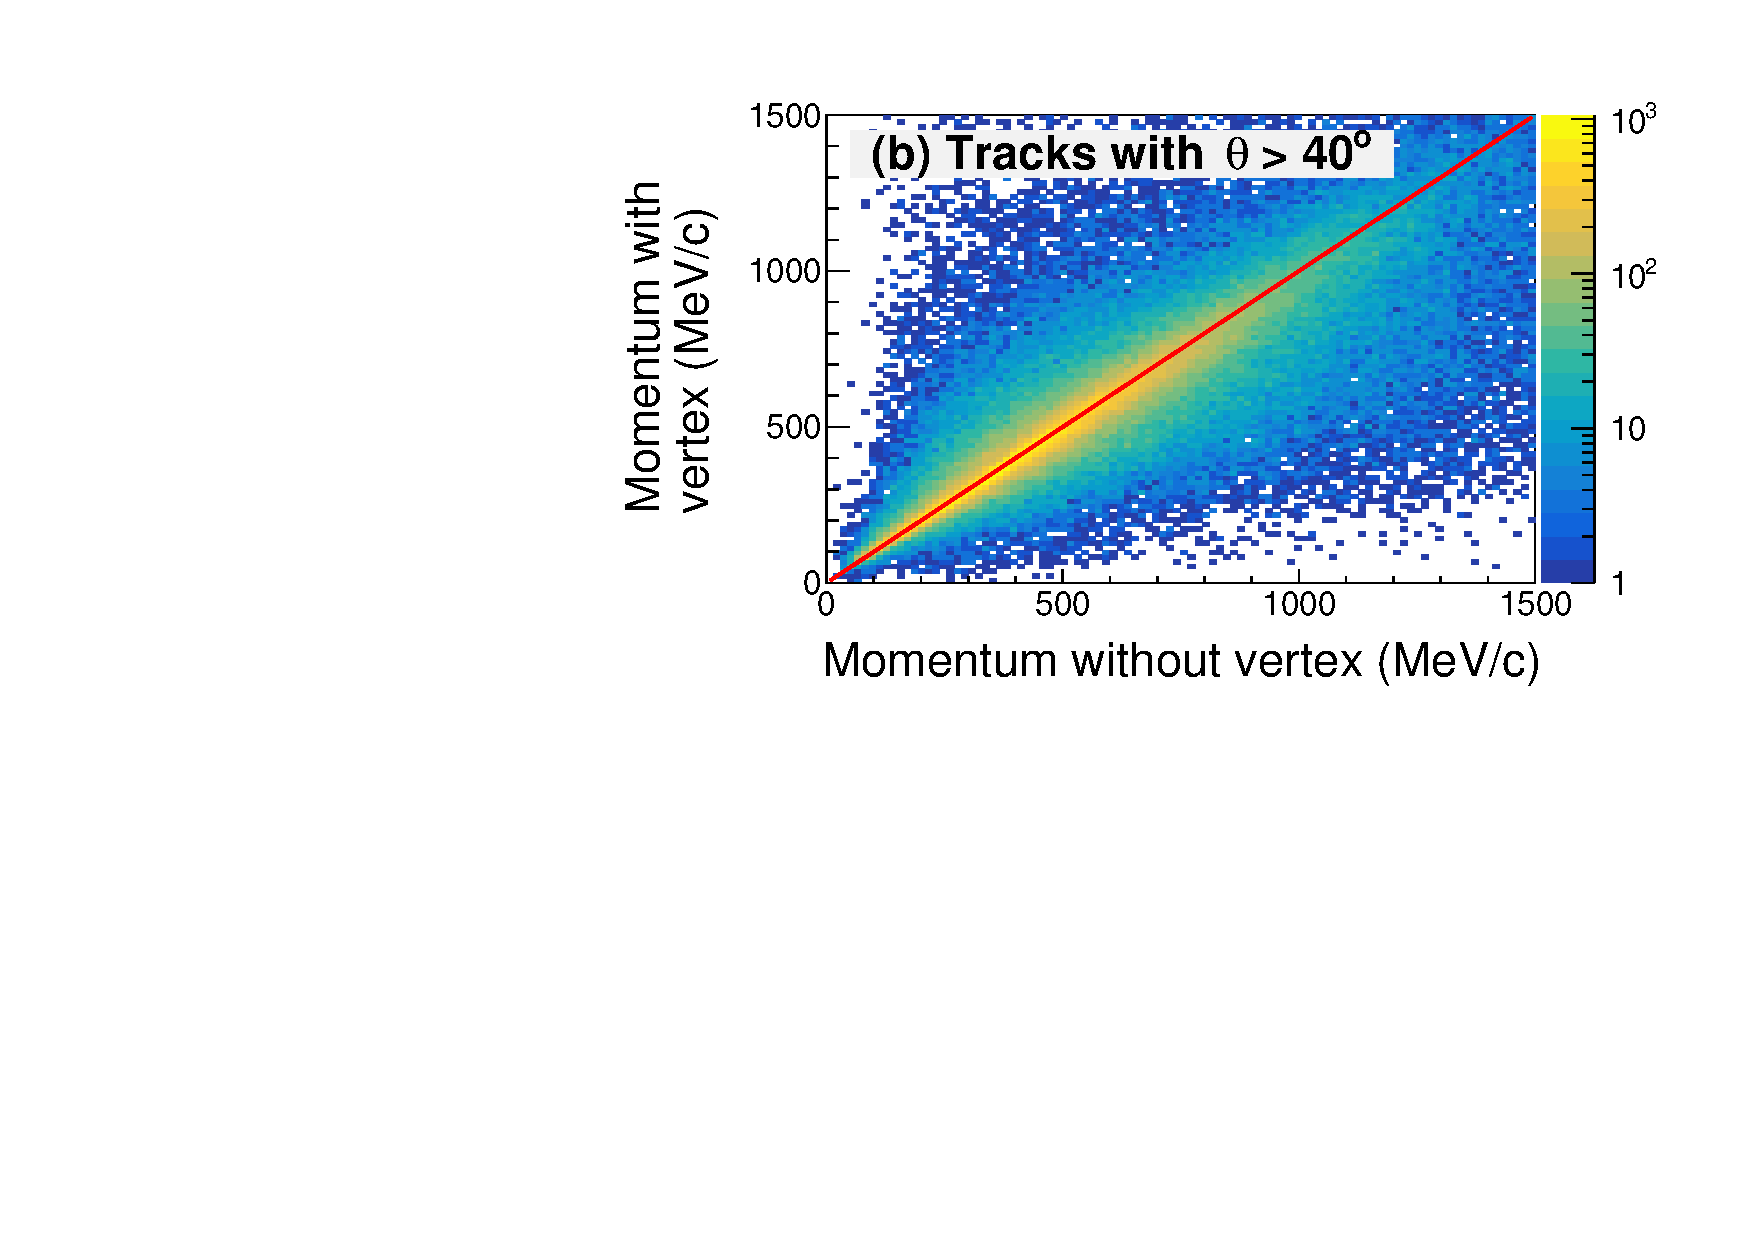
\includegraphics[width=\linewidth]{BDC_P_aftercor_large_angle.pdf} 
        \caption{Compare the momentum before and after including the BDC vertex for tracks with $\theta_{Lab} < \ang{40}$, after the space charge correction.} \label{fig:mom_L_after}
    \end{subfigure}
\label{fig:mom_sc}
\end{figure}



\begin{comment}

\begin{figure}[!htb]
    \centering
    \begin{subfigure}[t]{0.49\textwidth}
        \centering
        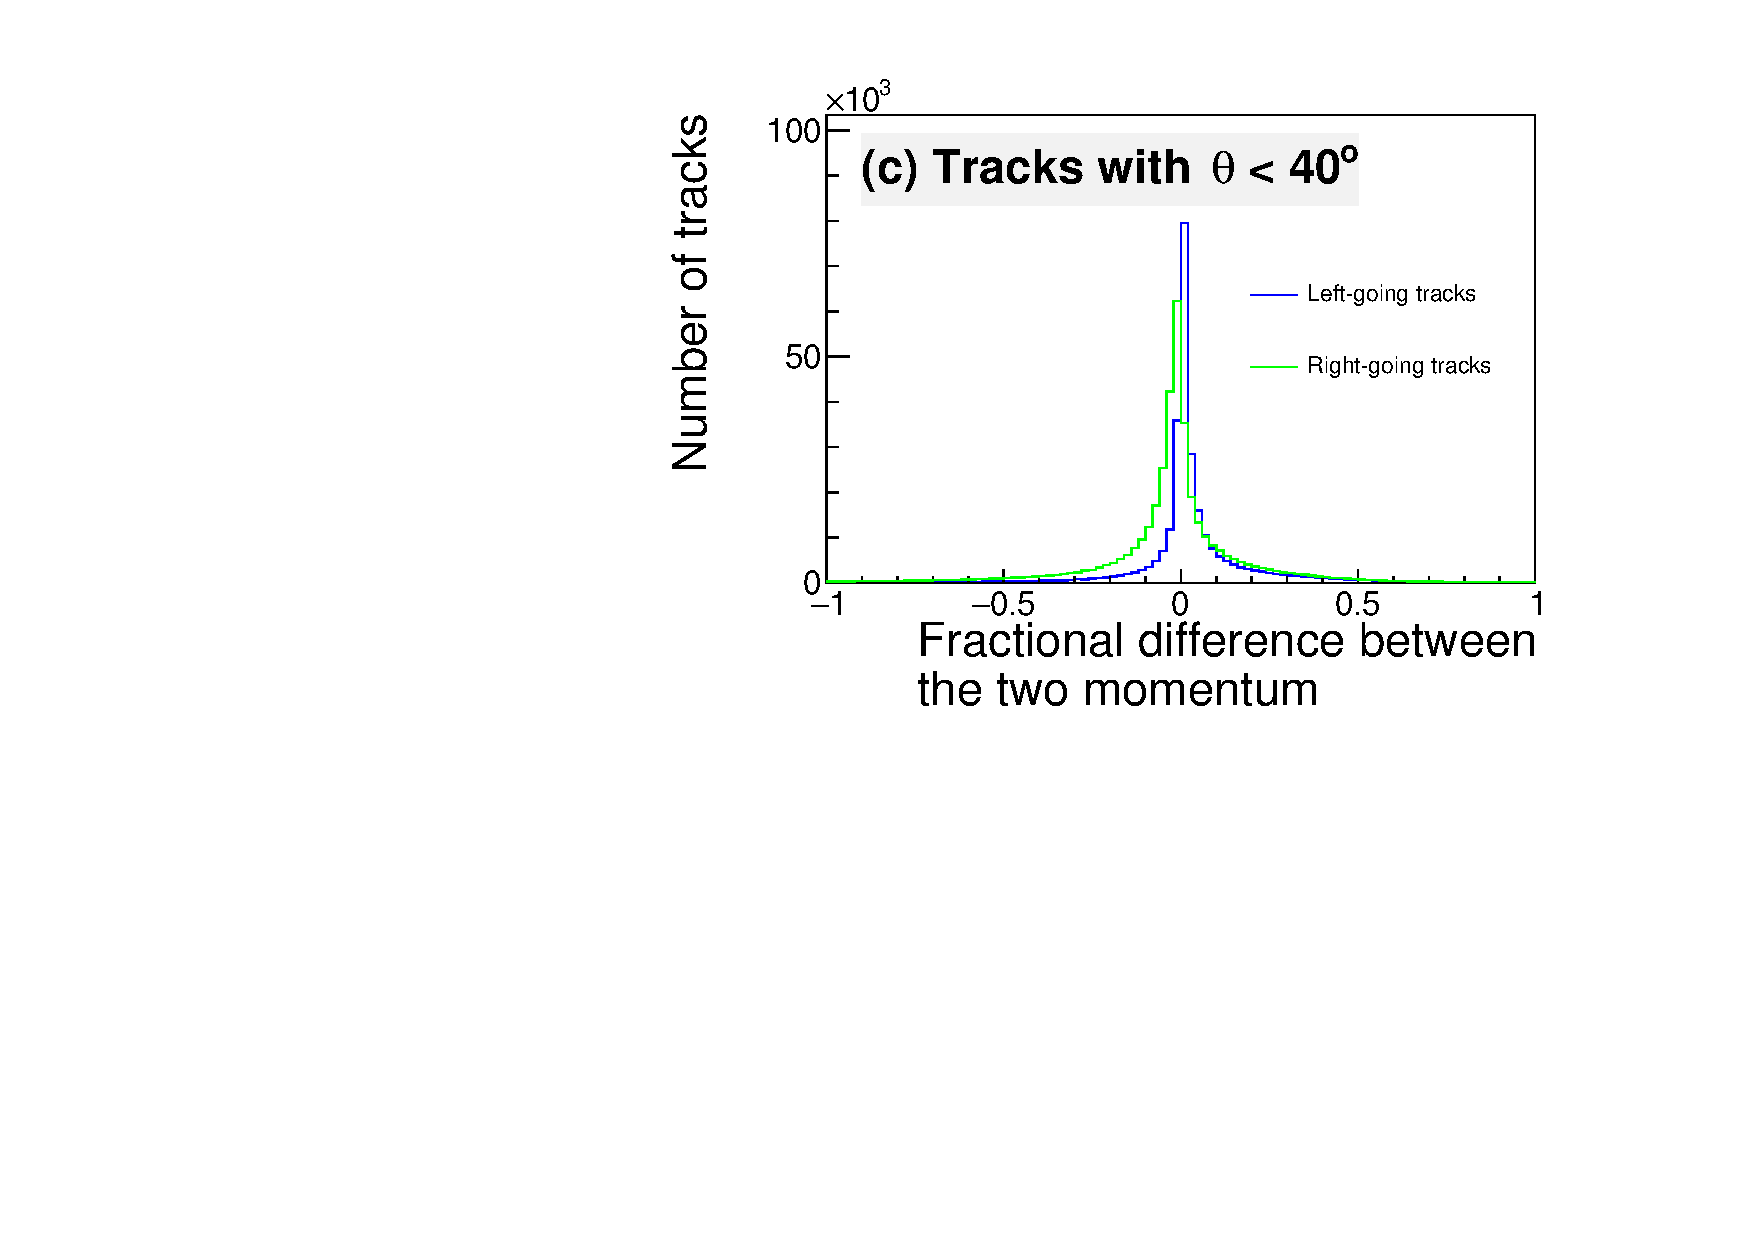
\includegraphics[width=\linewidth]{BDC_P_frac_small_angle.pdf} 
        \caption{Generic} \label{fig:mom_S_1D}
    \end{subfigure}
    \hfill
    \begin{subfigure}[t]{0.49\textwidth}
        \centering
        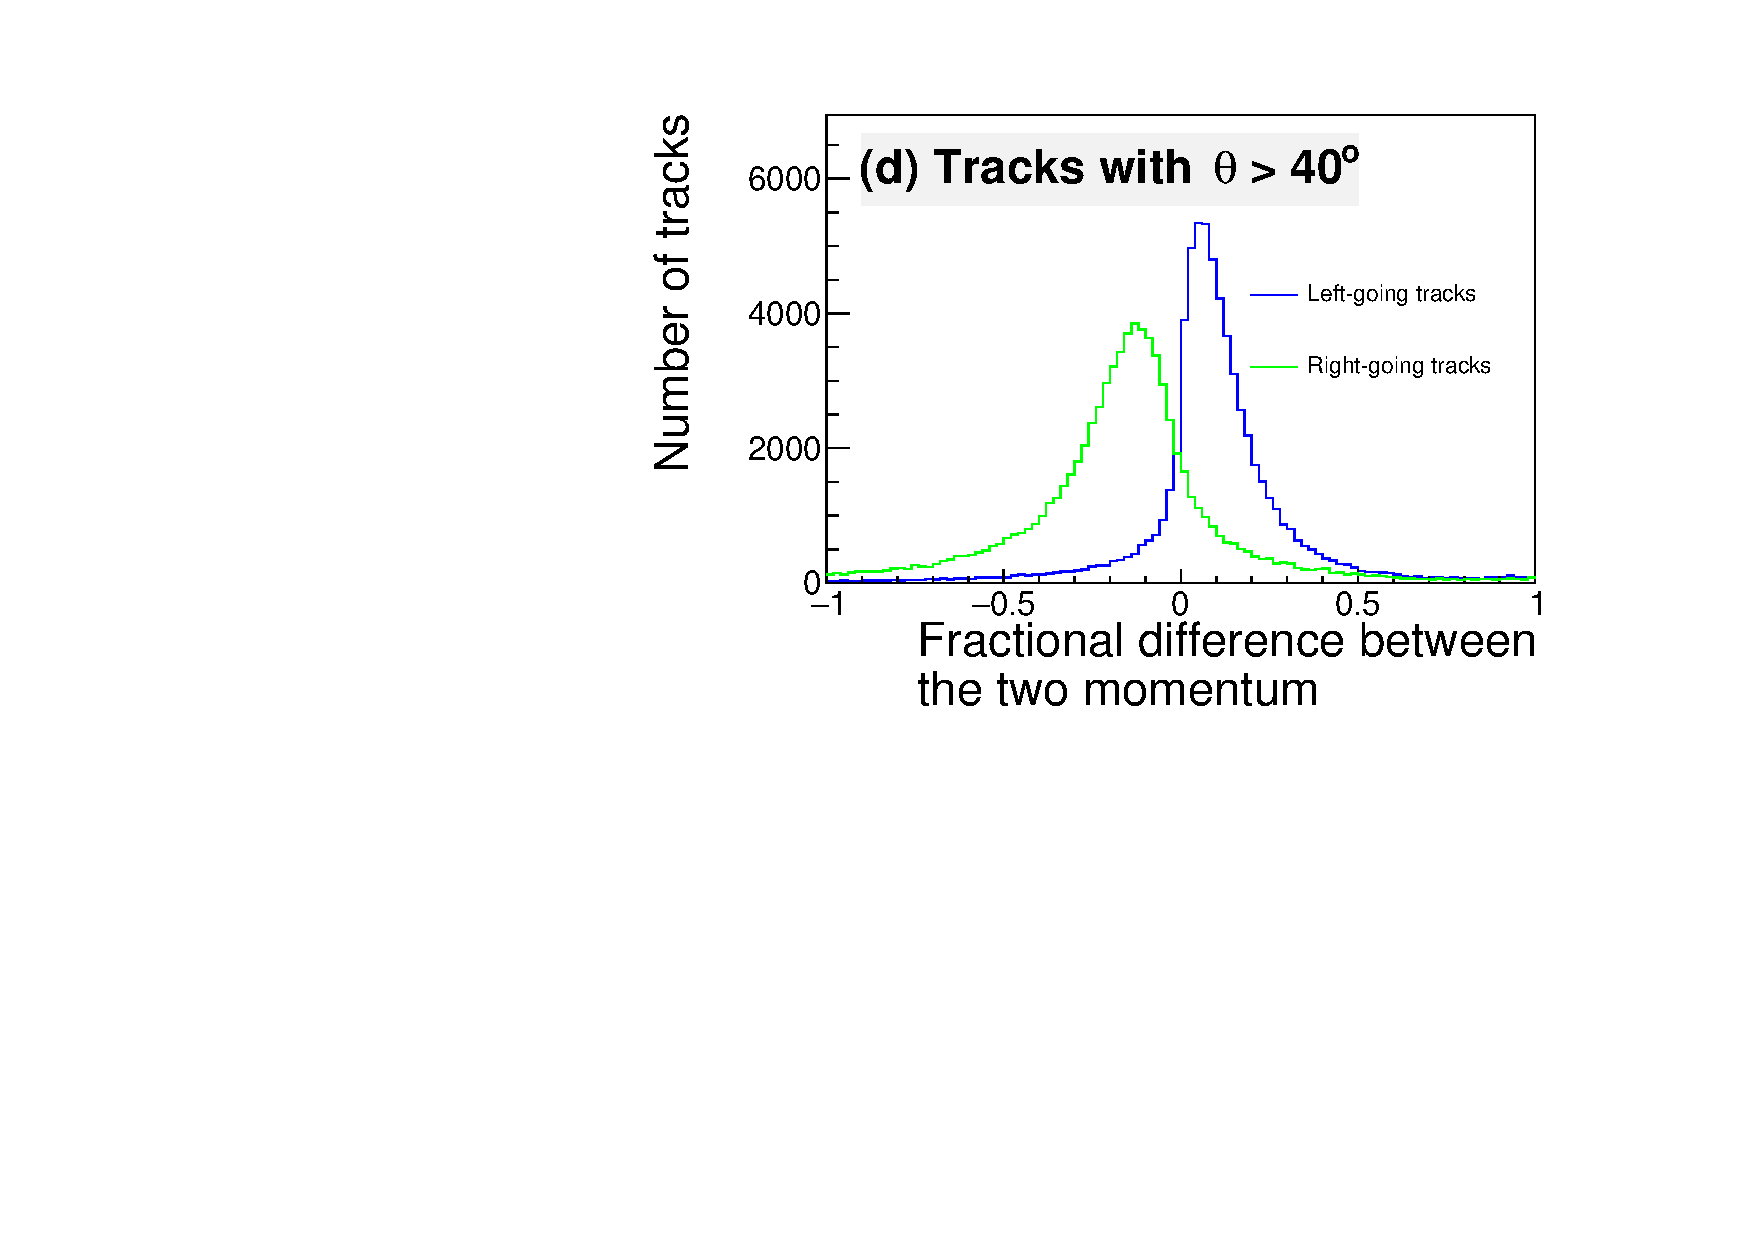
\includegraphics[width=\linewidth]{BDC_P_frac_large_angle.pdf} 
        \caption{Competitors} \label{fig:mom_L_1D}
    \end{subfigure}
    
\label{fig:mom_1D}
\end{figure}
\end{comment}






\begin{figure}[!htb]
    \centering
    \begin{subfigure}[t]{\textwidth}
        \centering
        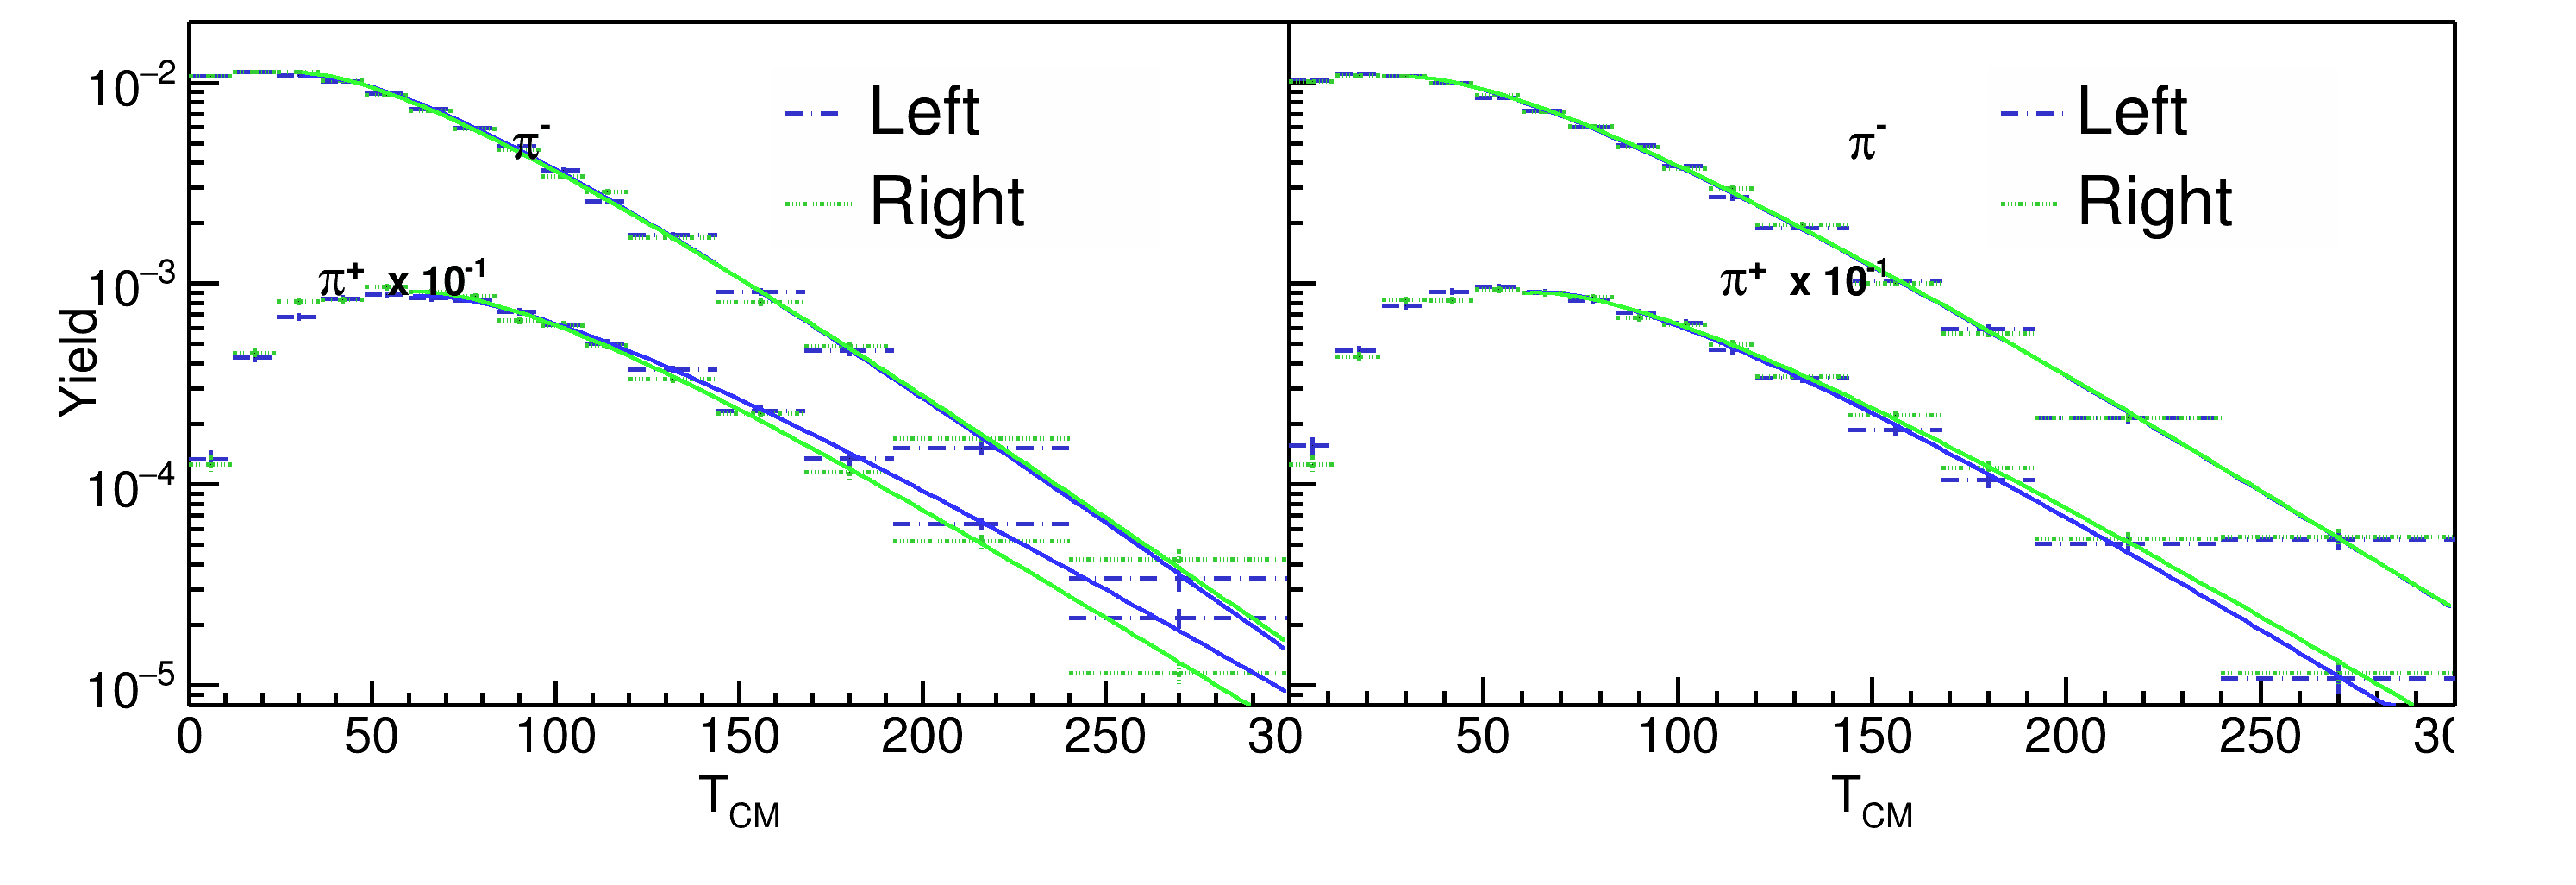
\includegraphics[width=\linewidth]{sn132_SC} 
        \caption{$\tin{132}{123}$ system.} \label{fig:132momdist_sc}
    \end{subfigure}
   
    \begin{subfigure}[t]{\textwidth}
        \centering
        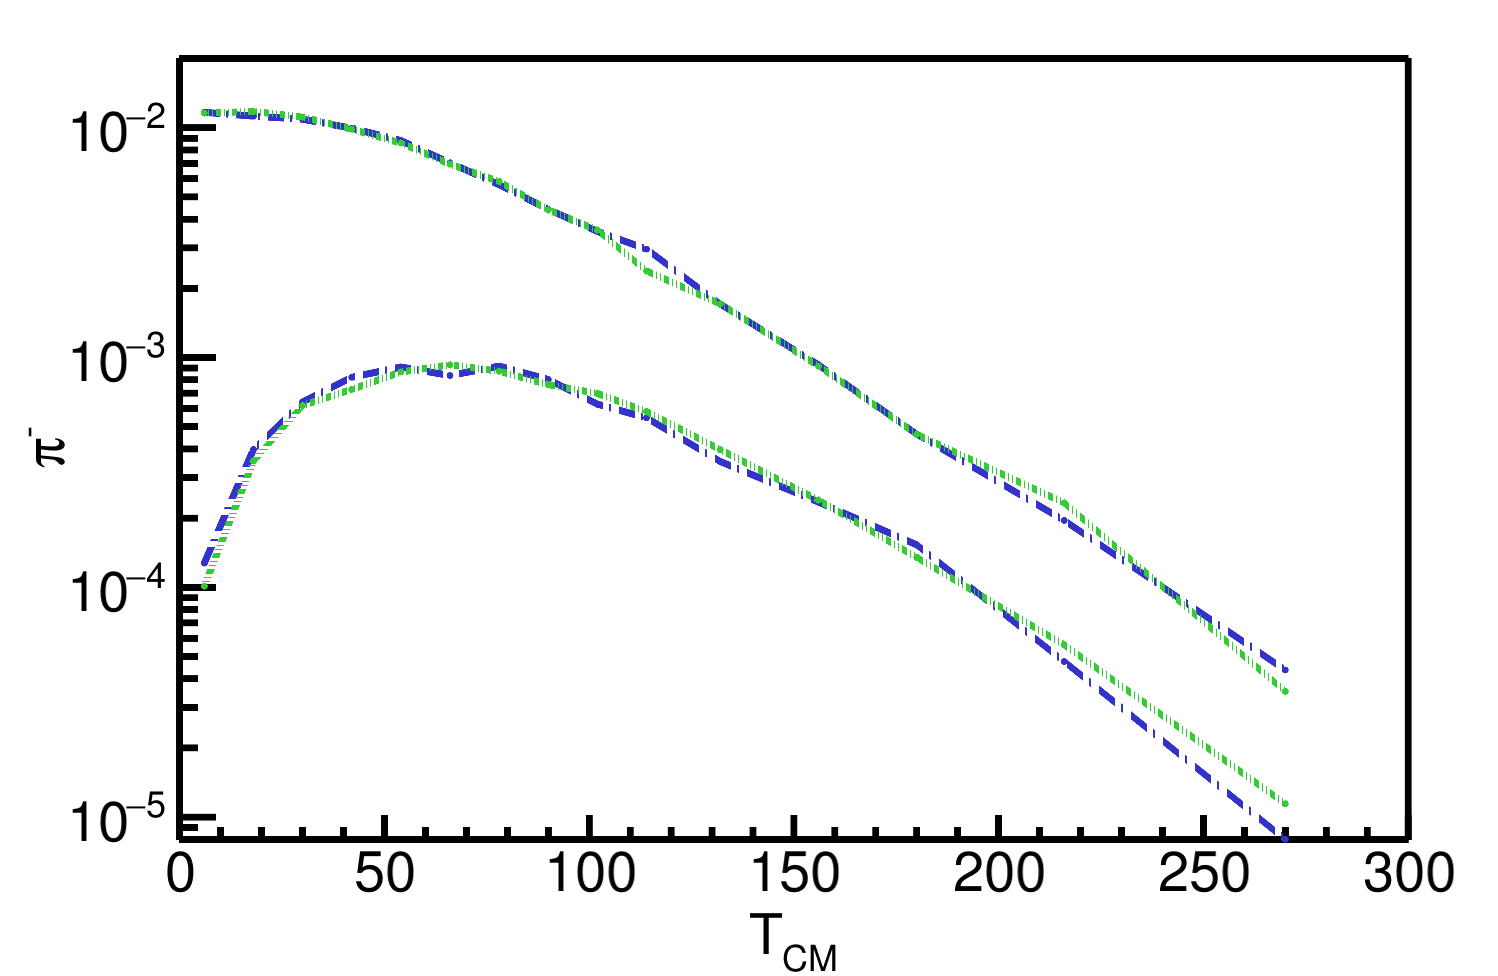
\includegraphics[width=\linewidth]{sn108_SC} 
        \caption{$\tin{108}{112}$ system.} \label{fig:108momdist_sc}
    \end{subfigure}
\caption{Momentum distributions of the Left and Right sides of the TPC for $\pi^+$ and $\pi^-$ particles.}
\label{fig:sc_momdist}
\end{figure}



Recall that only the relative distance between left and right-going tracks was minimized, and there was no guarantee that the corrected tracks coincide with the absolute BDC position at the target. This is one of the evidences of the correction's success. The others being the agreement with the expected cocktail calibration beam as described in Section~\ref{sec:cocktail}.

Here we will discuss some of the final results of the pion kinetic energy spectrum as it pertains to the verification of the space charge analysis,  the details of the pion PID analysis is discussed in detail in Section~\ref{sec:pid}. Figure~\ref{fig:sc_momdist} shows the $\pi^+$ and $\pi^-$ kinetic energy distributions in the center of mass system for the $\tin{132}{124}$ and $\tin{108}{112}$ systems. The momentum distributions are split into the beam-left and beam-right side of the TPC. In central collisions, one would expect no difference between the two momentum distributions due to the symmetry of the emission. Though as seen in the left panels of both figures, the data without the space charge correction is shown, where as in the right panel the data after the space charge correction is shown. There is a significant improvement in the matching of the left and right side momentum distributions for both particle species, in both systems.   It is remarkable that the dOCA observable which was used to calculate the amount of space charge was able to also correct the pion momentum distributions. There is no reason to assume correcting the dOCA distribution would be related to the momentum distribution, and is the strongest evidence to the success of the space charge correction.



\section{CoBo timing correction}
The arrival time of signals originating from each pad may differ due to timing delays in the electronics and cabling. The timing differences will affect the y-position measurement of each track. The y-direction track residuals reveal that the timing differences correspond to about $\pm$\SI{2}{\milli\metre} in position differences. The timing difference is stable for each pad across several runs.

\begin{figure}[!htb]
  \begin{center}
    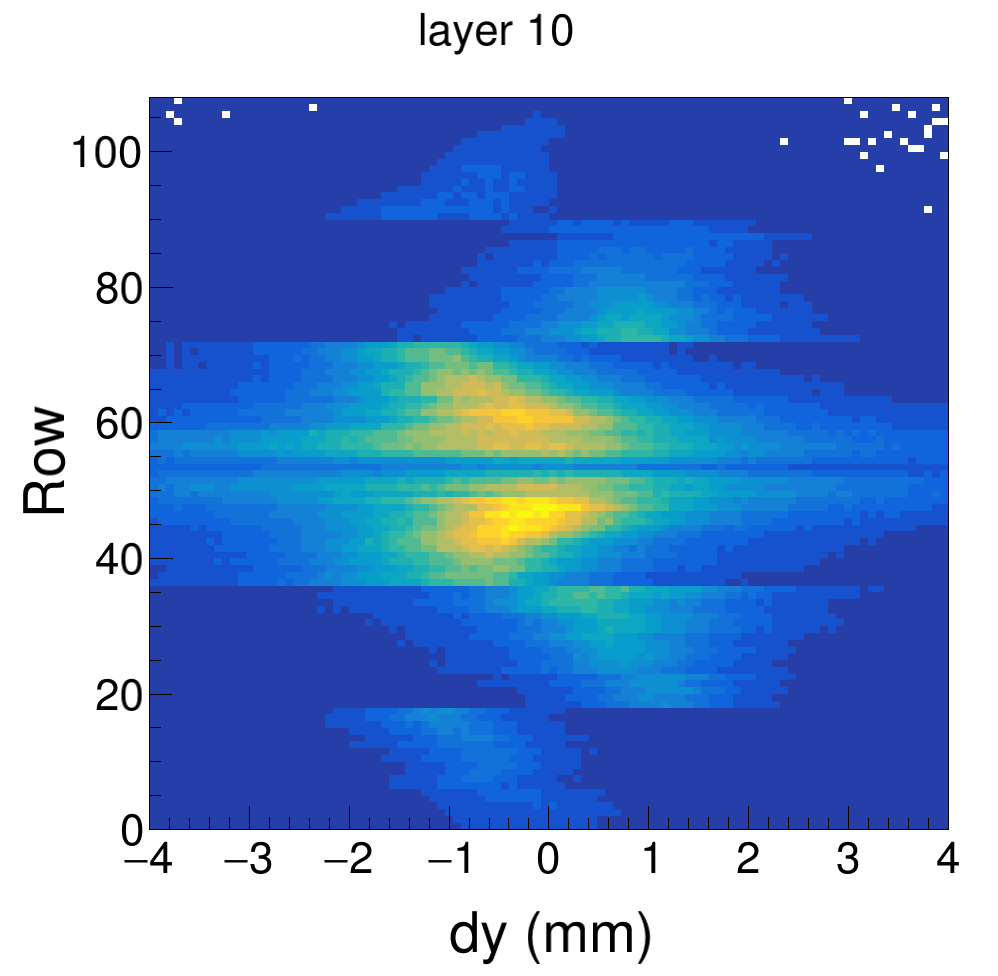
\includegraphics[width=0.33\textwidth]{run2907_yoffset6before_row_at_layer10.png}
    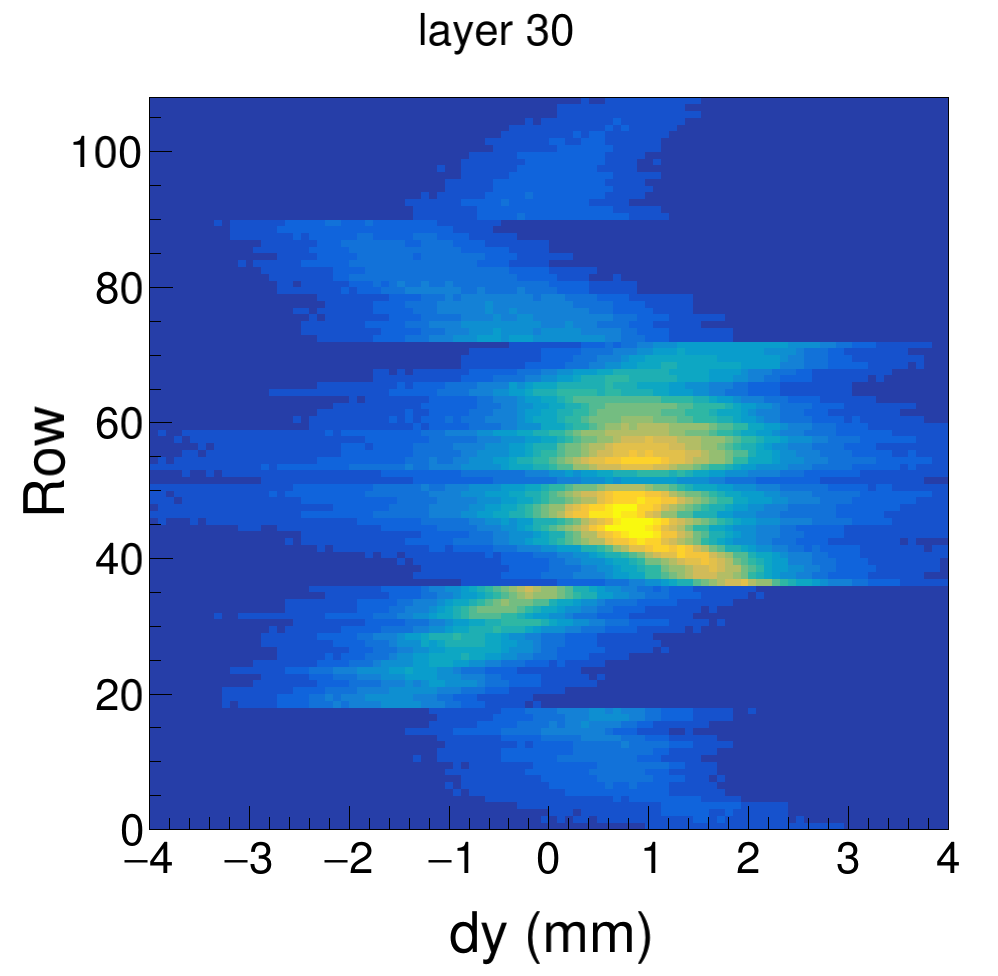
\includegraphics[width=0.33\textwidth]{run2907_yoffset5before_row_at_layer30.png}
    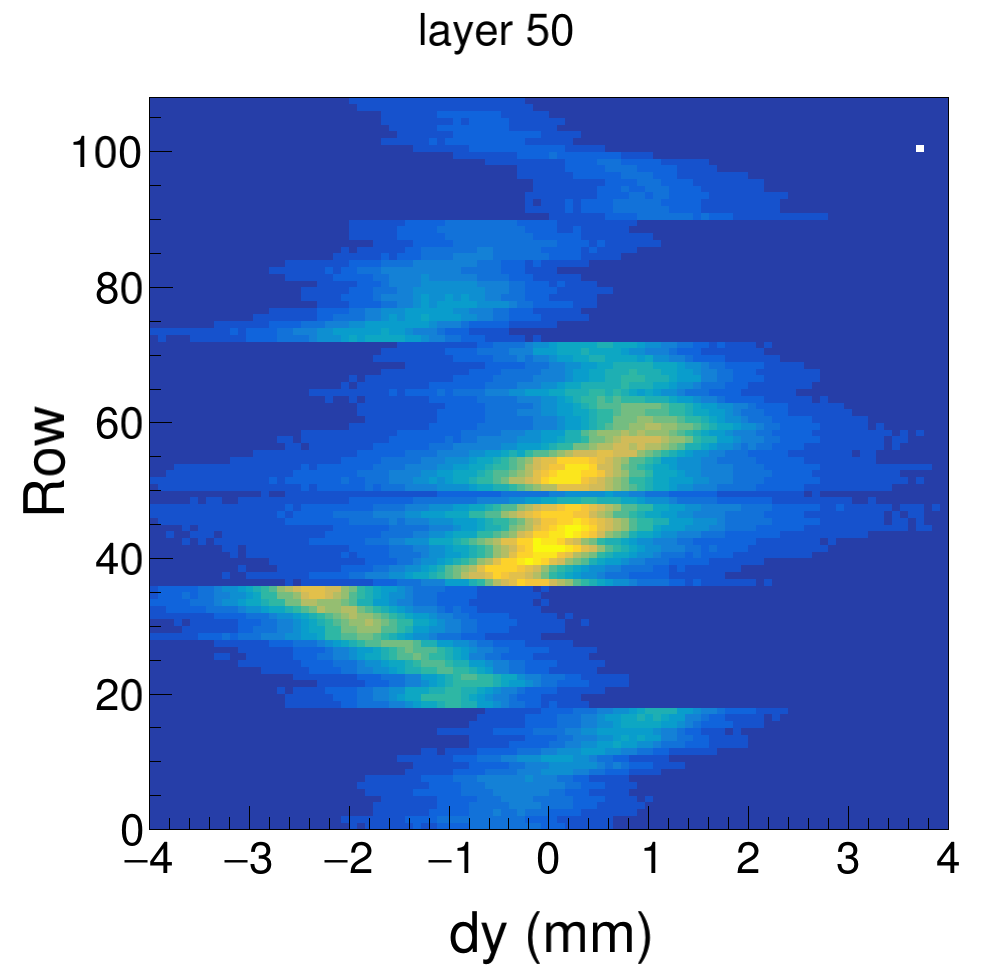
\includegraphics[width=0.33\textwidth]{run2907_yoffset4before_row_at_layer50.png}
 
    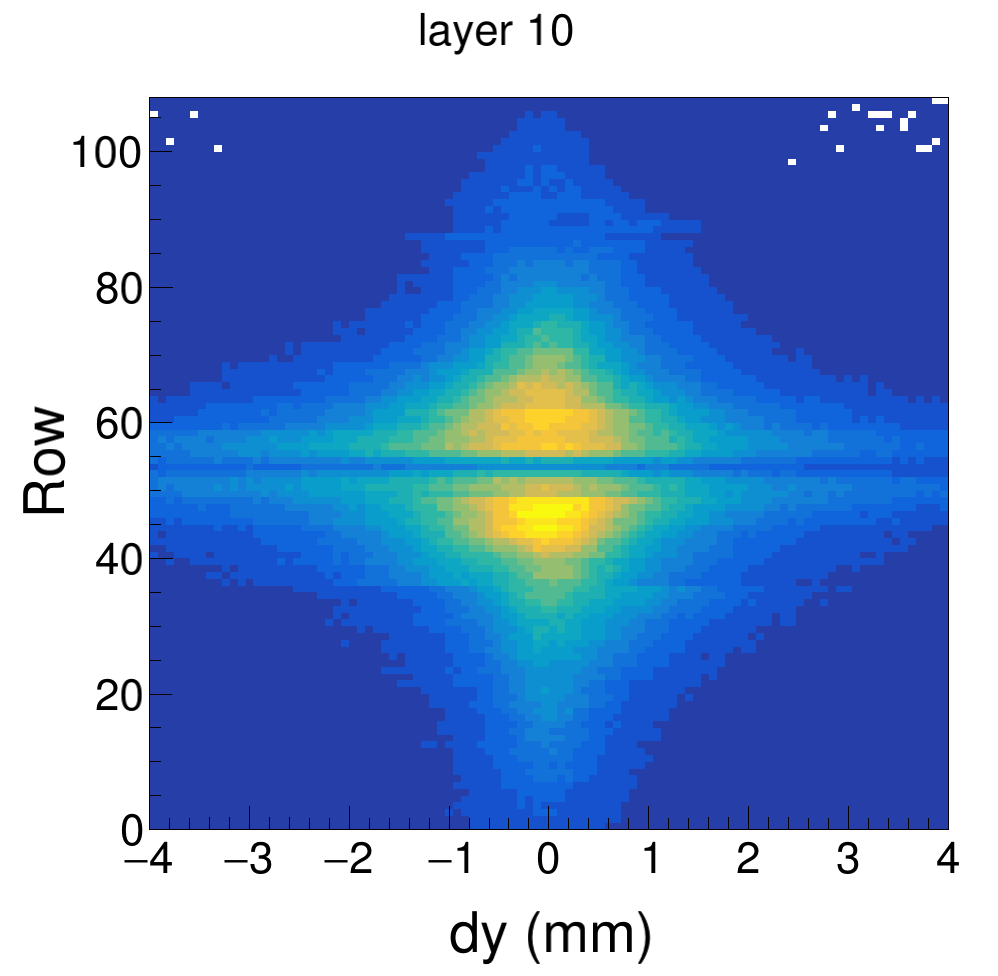
\includegraphics[width=0.33\textwidth]{run2907_yoffset6after_row_at_layer10.png}
    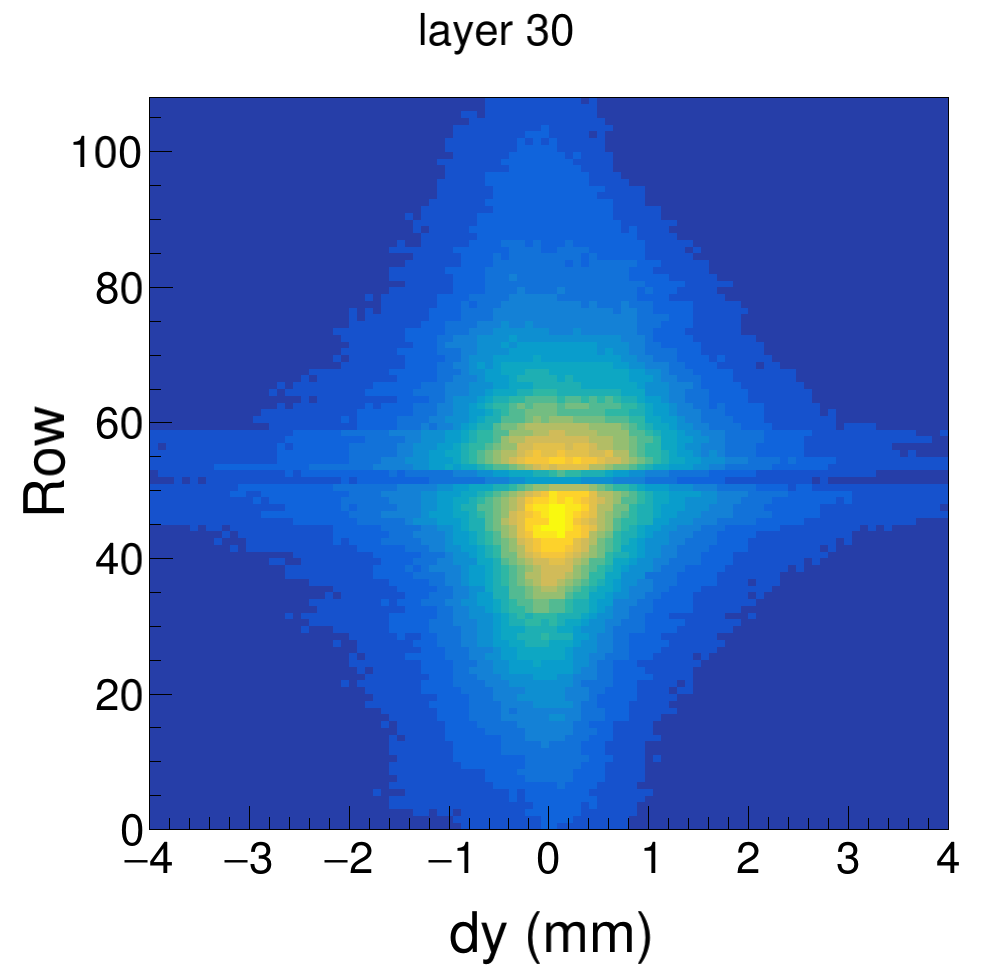
\includegraphics[width=0.33\textwidth]{run2907_yoffset5after_row_at_layer30.png}
    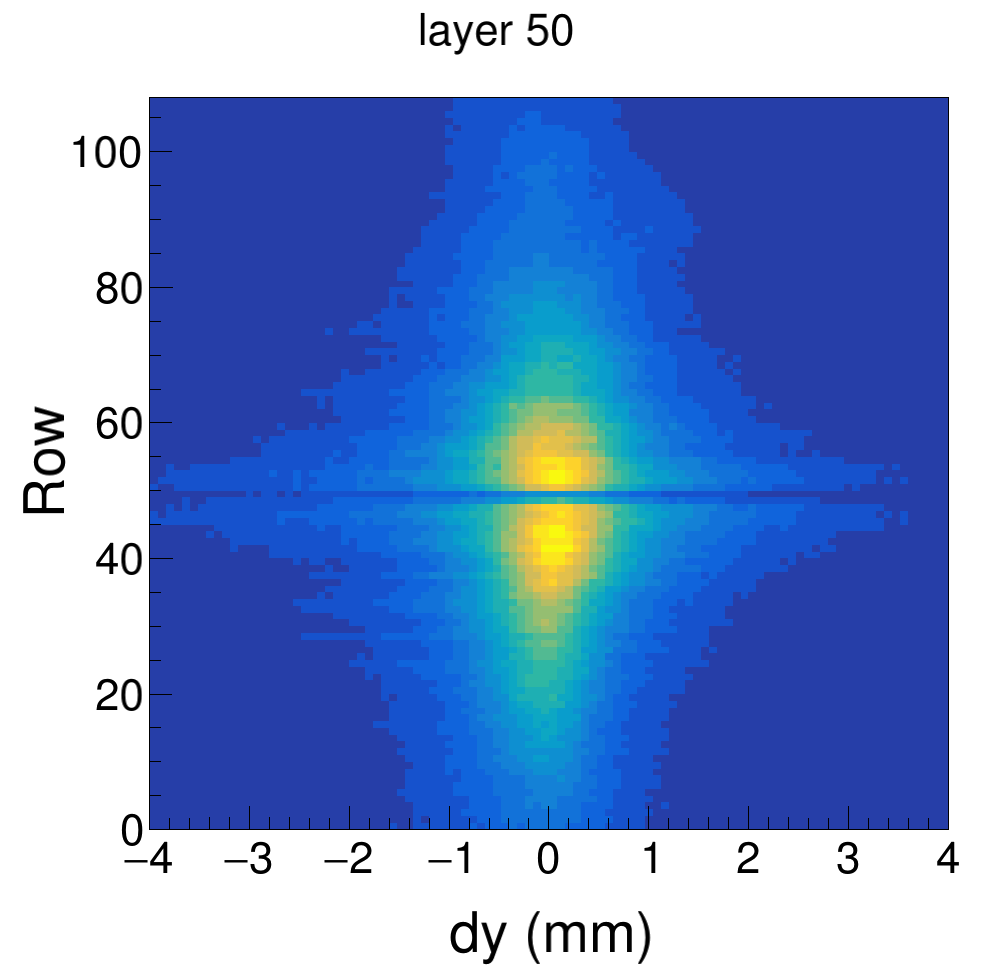
\includegraphics[width=0.33\textwidth]{run2907_yoffset4after_row_at_layer50.png}
 
  \end{center}
  \caption{Cobo timing correction.}
  \label{fig:coboCorr}
\end{figure}



\begin{figure}[!htb]
    \begin{subfigure}[t]{.49\textwidth}
        \centering
        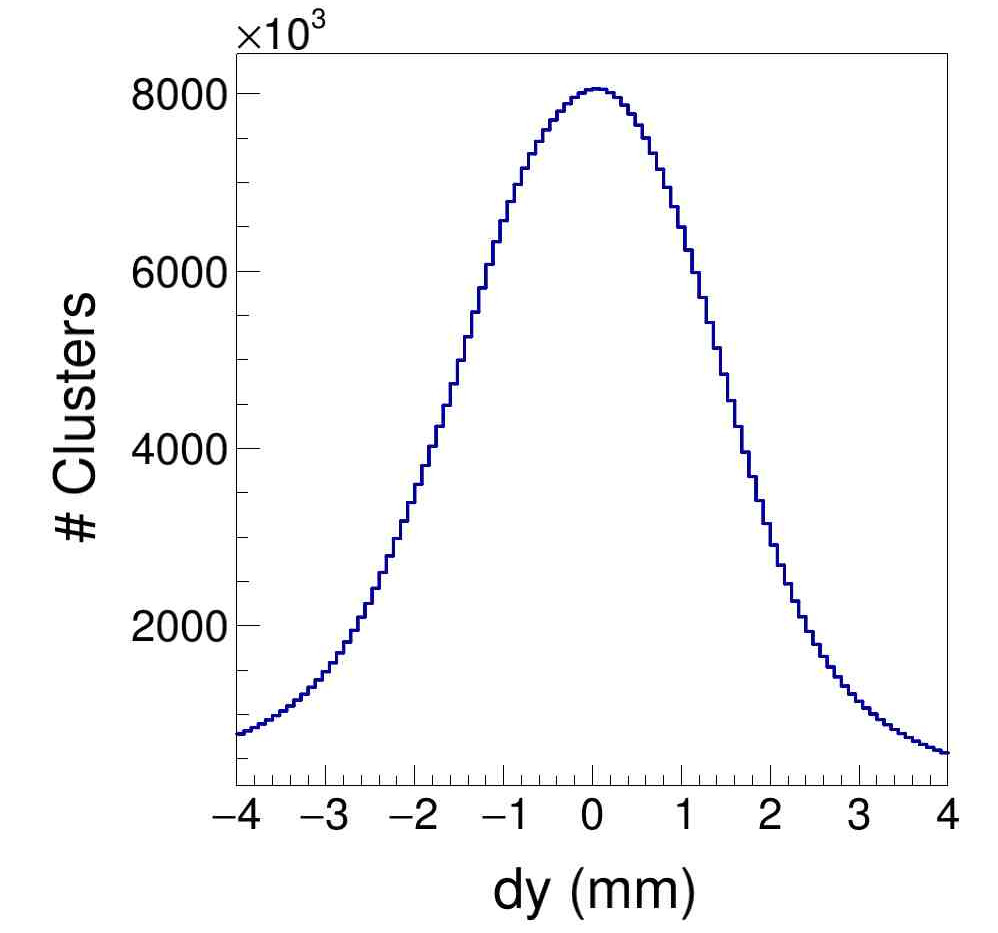
\includegraphics[width=\linewidth]{run2905_yoffset1before_all.jpg} 
        \caption{Y-residual distribution for all pads before correction.} \label{fig:yoff_allBefore}
    \end{subfigure}
    \hfill
    \begin{subfigure}[t]{.49\textwidth}
        \centering
        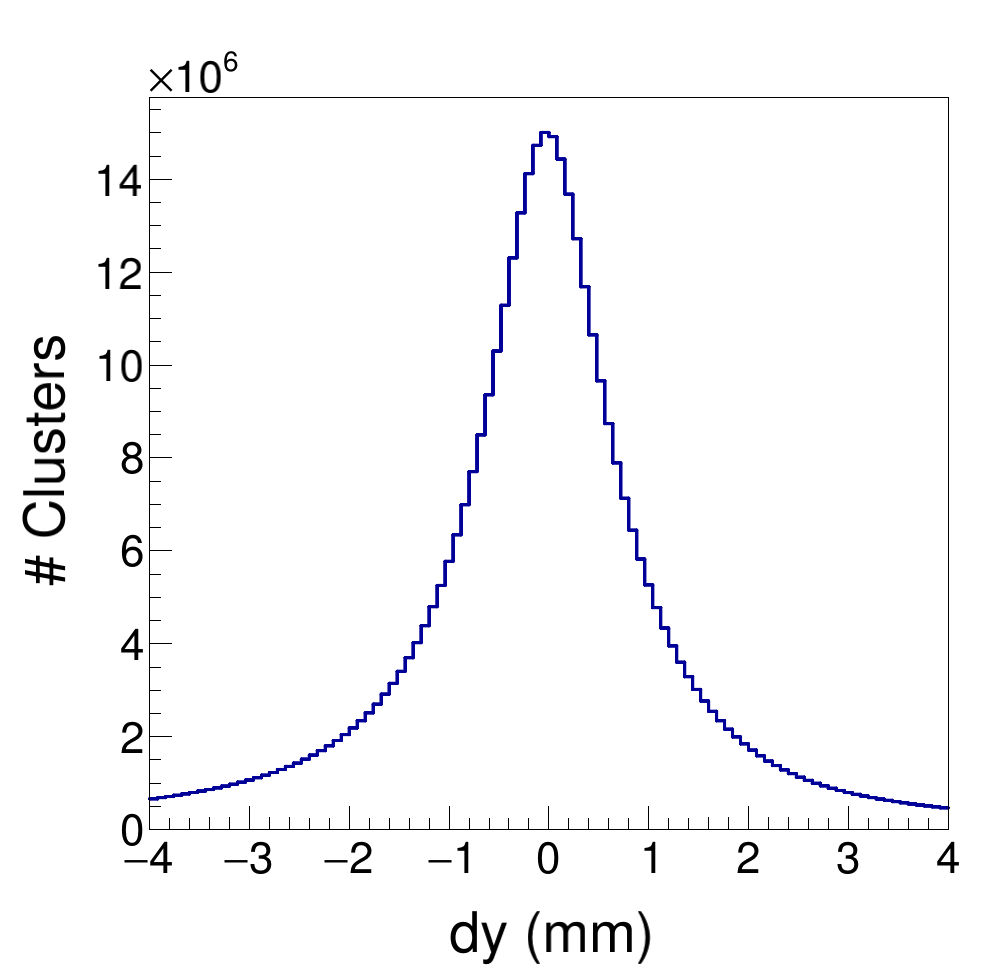
\includegraphics[width=\linewidth]{run2905_yoffset1after_all.png}
        \caption{Y-residual distribution for all pads after correction.} \label{fig:yoff_allAfter}
    \end{subfigure}
    \caption{ }
\label{fig:yoff}
\end{figure}


 Figure~\ref{fig:coboCorr} shows the y-residuals, across all the rows, for three different layers. Before the correction, one can see large deviations in the y-residuals which correspond to timing differences. The mean value of the y-residual distribution is fitted and an inverse correction map is constructed for each pad. The data is then reconstructed subtracting value from the inverse map, $dy$, for each pad. The resulting corrected distribution is shown in Fig.~\ref{fig:coboCorr} for the same layer set. Figure~\ref{fig:yoff} also show the summary of all the pads before the correction and after the correction. There is a significant improvement in the width of the distribution going from \SI{1.5}{\milli\metre} to \SI{0.6}{\milli\metre}. 



%Reference appendix for poisson solver 
%Tables for ion drift velocity in P-10 Gas reference Sauli
%Figure of sDAC or POCA 
%Figure of cartoon of what is happening to tracks
%Figure of correction map in TPC and MC map 
%Figure of before and after correction BDC vs reco momentum
%Figure of track residuals before and after?



\section{Monte Carlo Simulation}
The MC simulation is composed of two separate simulations. The first simulation models the interactions of a particle passing through the various materials in the TPC using Geant4. A scale model of the field cage, and its materials, where the gas mixture is P-10 gas at a density of 1 atm. The magnetic field map of the SAMURAI dipole magnet was imported into Geant4 as well after assuming rotational symmetry along the axis perpendicular to the pole face. Along with the energy loss and particle transport, Geant4 also handles multiple scattering, and particle decay, which are all important effects for pions. The output of Geant4 is a series of energy loss points which contain the amount of energy lost in $\si{\kilo\electronvolt\per\centi\metre}$ and the location of the energy loss in Cartesian space $(x,y,z)$. 

In the second part of the MC simulation, the physical processes of the TPC measurement are simulated, such as the electron drift, avalanche process, and all processes involved in the signal creation in the electronics. This is separated into three software tasks, the drift, pad response, and electronics tasks. In the following section we will discuss these tasks in more detail, the discussion of Geant4 is not covered here and the reader is refered to \cite{geant4}.  

\subsection{Drift Task}
 
 The first step of the drift task is to convert the primary ionization points of the MC track provided by Geant4 into electrons. The average number of electrons created in a gaseous detector,$N_{e^-}$, can be described as,
\begin{equation}
N_{e^{-}} =  \frac{\Delta E}{I},
\label{eq:kev2el}
\end{equation}
 
where $I$ is the ionization coefficient of P10 gas (Table~\ref{tb:gas}) and $\Delta E$ is the energy loss deposited. Each electron is propagated along the electric field lines assuming the electric field is uniform, which is true for mos tof the pad plane region. The total length drifted from the initial primary ionization point to the final anode wire is given by $L_{anode}$. 

\begin{table*}\centering
\ra{1.3}
\begin{tabular}{@{}rr@{}}\toprule 
\multicolumn{2}{c}{Electron Transport Gas Properties} \\
 \midrule
Drift velocity & 5.53 $\si{\centi\meter\per\micro\second}$\\
Transverse diffusion & 240 $\si{\micro \meter \centi\meter}^{-1/2}$\\
Longitudinal diffusion &  340 $\si{\micro \meter \centi\meter}^{-1/2}$\\
Gas Ionization & 26.2 $\si{\eV}$\\
\bottomrule
\end{tabular}
\caption{An overview of electron drift properties in P10 gas.}
\label{tb:gas}
\end{table*}

Drifting electrons frequently collide with the detector gas causing them to change direction. This stochastic motion is  described by a a diffusion process occurring along the direction of travel (longitudinal) and transverse to the motion. The longitudinal ($c_{l}$) and transverse ($c_{t}$) diffusion coefficients are determined by Garfield++ calculation  \cite{garfield++} in the presence of a \SI{0.5}{\tesla} magnetic field, listed in Tb.~\ref{tb:gas}. The diffusion process is modeled by randomly sampling from a Gaussian distributions describing both of the directions. The random displacement vector is then added to the final position of the electron. The deviation in the transverse direction, $dr$, is randomly sampled from,

\begin{equation}
dr = e^{-\frac{r^2}{2\sigma_{t}^2}},
\end{equation}

where $\sigma_{t}=c_{t}\cdot\sqrt{L_{anode}}$.The Cartesian directions are given by $dx = dr \cdot \cos(\alpha)$ and $dz = dr \cdot \sin(\alpha)$, where $\alpha$ is a random angle from 0 to 2$\pi$, since there is no preferential angle  of emission in the transverse plane. The shift associated with the longitudinal diffusion, $dl$, is randomly sampled from, 

\begin{equation}
dl = e^{-\frac{t^2}{2\sigma_{l}^2}},
\end{equation}

where $\sigma_{l}=c_{l}\cdot\sqrt{L_{anode}}$. 

The final position of the electron along the wire is calculated  $x' = x + dx$. The electron will terminate on the closest anode wire, that is the anode wire that is closest to the shifted z-position $z\textprime = z + dz$, and the final electron z position is then updated to be the same as the anode wire it terminated on. The total drift time of the electron $t$ is calculated as,

\begin{equation}
 t = \frac{L_{anode} + dl}{v_d} + t_{offset},
 \label{eq:electronTime}
\end{equation}
 
where $v_d$ is the drift velocity. The parameter $t_{offset} = \SI{49.92}{\nano\second}$ is to allow for an alignment of the MC time bucket spectrum with the data. This is because the y-position corresponding to $t=0$ in the data time bucket spectra, does not correspond to the same position in the MC.  This value was found to be \SI{23}{\nano\second} by aligning the MC vertex to the data vertex.

The total number of electrons produced in the avalanche process of a single electron was simulated in Garfield++ and discussed in Section~\ref{sec:wireplanes} for the anode wire voltages used in the experiment. The number of electrons produced in the avalanche is randomly sampled from the distribution depending on which anode wire section the electron terminated. The number of electrons produced is stored as a gain factor instead of multiple instances of the original electron to save space and computation time. 

%We assume that the lateral movement along the wire arising form $\vec{E}\times\vec{B}$ effect near the wire is negligible as compared with diffusion and other effects described later. 

It is worth mentioning there is the possibility to simulate the space charge effects in this task where as the inverse to the correction map described in Section~\ref{sec:spacecharge}. This is not used for calculating the response of the TPC for efficiency calculations since it is a trivial exercise to input the space charge map only to then correct for it using the inverse map.  

\subsection{Pad Response Task}
The total charge of each avalanche is distributed according to the pad response function (PRF) described in Section~\ref{sec:prf}. The PRF is simulated as the double integral of a 2-dimensional Gaussian. The final output charge on all the pads are the superposition of the PRFs of all drifted electrons. The MC PRF is expressed as, 

\begin{equation}
PRF(x,z) = \iint e^{-\frac{(x-x_o)^2}{2\sigma_x^2}} e^{-\frac{(z-z_o)^2}{2\sigma_z^2}}dxdz,
\end{equation}

where $\sigma_x = 3.4$ and $\sigma_z = 3.5$, and $x_0$ and $z_0$ are the final position of the drifted electron. The parameters were determined through an iterative comparison matching the PRFs of the MC and experimental data sets. 


\subsection{Electronics Task}

The purpose of the electronics task is to simulate the electronics response to charge induced on each pad, converting charge into ADC channels. The induced charge on each pad goes through a pre-amplifier and shaping amplifier which determine the final pulse shape that is read out. The pulse shape did not change significantly in any circumstance, such as pulse height, data type, or particle type, as long as the electronics settings are fixed. This allows us to assume the pulse shape is constant and can be described by two variables, the height of the pulse, $Q$, and the starting time bucket of the pulse, $t_o$. The starting time of the pulse is defined as the time at .1$\cdot Q$ of  the rising edge. The shape of the pulse depends on the shaping time constant which was set to \SI{117}{\nano\second} for the data analyzed here. Figure~\ref{fig:pulseshape} shows the pulse shape which was extracted from the experimental signals in the data. These were signals that did not saturate the electronics and was averaged over a wide range of ADC values. Here it is normalized so the maximum height is 1. 



\begin{figure}[!htb]
    \centering       
    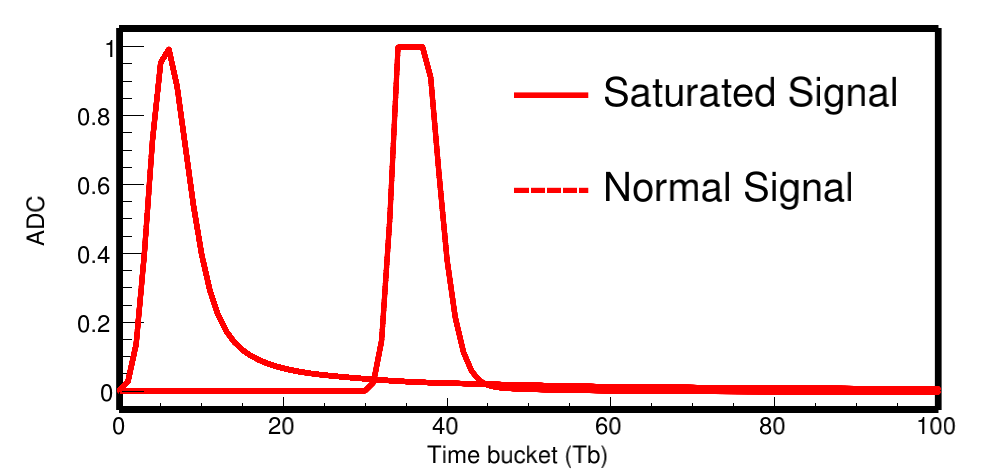
\includegraphics[width=\linewidth]{satpulse.png} 
    \caption{The standard pulse shape and saturated pulse shape extracted from the experimental data, and used in the MC software.}
    \label{fig:pulseshape}
\end{figure}


Converting the charge in each pad into the height of the ADC response in the electronics is calculated as, 

\begin{equation}
Q = f_G  N_{e}  \cdot e \cdot\frac{ADC_{max} - ADC_{pedestal}}{f_c}
\label{eq:etoADC}
\end{equation},

where $e$ is the charge of the electron in $\si{\femto \coulomb}$, $N_{e}$ is the total number of avalanche electrons, $ADC_{pedestal}$) is the pedestal (300 ADC, $\mathrm{ADC_{Max}}$ is the maximum allowed ADC value (4096), and $f_c$ is the dynamic range setting (\SI{120}{\femto\coulomb}). The pulse shape given in Fig.~\ref{fig:pulseshape} is multiplied by the pulse height $Q$ giving the full time bucket estimate of the TPC response. Random Gaussian noise is added to each time bucket, where the root-mean-squared value of the electronics noise was measured to be around 6 ADC. The timing information of the pulse is calculated from Eq.~\ref{eq:electronTime}. The coefficient $f_G$ corresponds to a factor which allows for fine tuning of the ADC calibration. This factor is calculated by

\begin{equation}
f_G^p = \frac{\langle dE/dx\rangle_{Data}^p}{\langle dE/dx\rangle_{MC}^p}
\label{eq:dedxcalibration}
\end{equation}

where $\langle dE/dx\rangle_{MC}^p$ and $\langle dE/dx\rangle_{Data}^p$  are the energy loss values for a particle in a given momentum bin $p$. The calibration will be discussed later in more detail. 


\section{Monte Carlo Track Embedding}
\label{sec:embedding}
Track embedding is the process of taking a MC simulated track and embedding its response into an experimental data event. After reconstructing this new embedded event we match the input MC track to the corresponding final reconstructed track.  By doing so we can evaluate the response of the entire TPC system to any given input. The TPC measurement can be thought of three different systems each which introduce errors and or biases into the final reconstructed tracks; the software, the detector, and the experimental setup. The 

There are several effects in a complex experimental set up that influence the data in either unknown or un-quantifiable ways. One such effect is the bias of the triggering system, here the Kyoto and Katana multiplicity and veto arrays preferentially select data that is emitted in a particular reaction plane. As previously discussed saturation effects in the electronics, notably the shadowing of other tracks. The effects of track multiplicity and the distribution of heavy ion and residues from the breakup of the target and projectile. One could propose to make a simulation or investigation into each individual effect in order to make a full MC simulation of data and study the response of the detector this way. Though great care was taken in developing an accurate MC simulation, like all models there are assumptions and simplifications that were made. Simply put, there is no better substitute for experimental data than itself. By embedding MC tracks into experimental data -- and propagating through the tracking and reconstruction algorithm -- one can account for all these sources of biases which are contained in the experimental data, while at the same time measuring the response of the TPC.

As discussed in Section~\ref{sec:software}, the software is composed of several tasks, each of which have the possibility of introducing errors or biases through assumptions made in the tracking algorithm. The detector system introduces errors related to the physical measurement itself which can be addressed through modeling the TPC, and its materials. 

For all of the sources of biases in the TPC, it is clear that a MC type approach to solving for the response of the TPC would be the most practical method. Also by embedding MC events into real data we can take into account the effects of the experimental setup as well as the software and the detector system all together at once. 

%\begin{sidewaysfigure}[!htb]
%\centering
%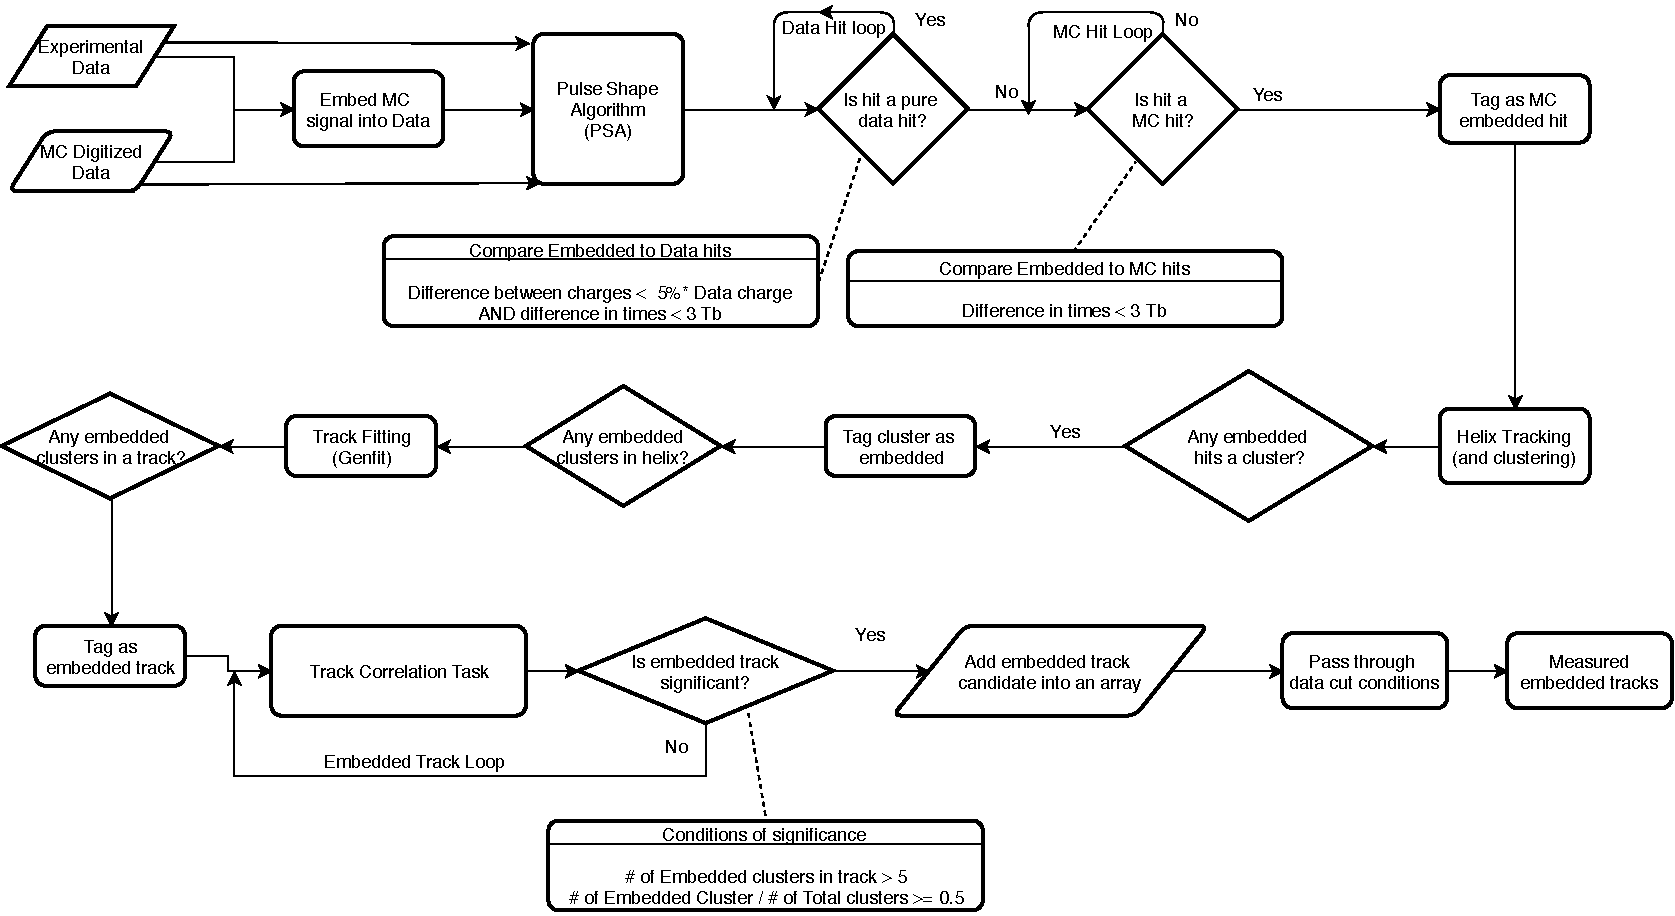
\includegraphics[width=\textwidth]{FlowEmbedding.pdf}
%\caption{Flow of embedding implementation in the software.}
%\label{fig:flow}
%\end{sidewaysfigure}


%\clearpage
%\pagestyle{lscape} % first clear the page and change the pagestyle
%\begin{landscape}
% your landscape table(s) or figure(s) here
%CONSIDER ROTATING THIS FIGURE IF ALLOWED
\begin{figure}[!htb]
\centering
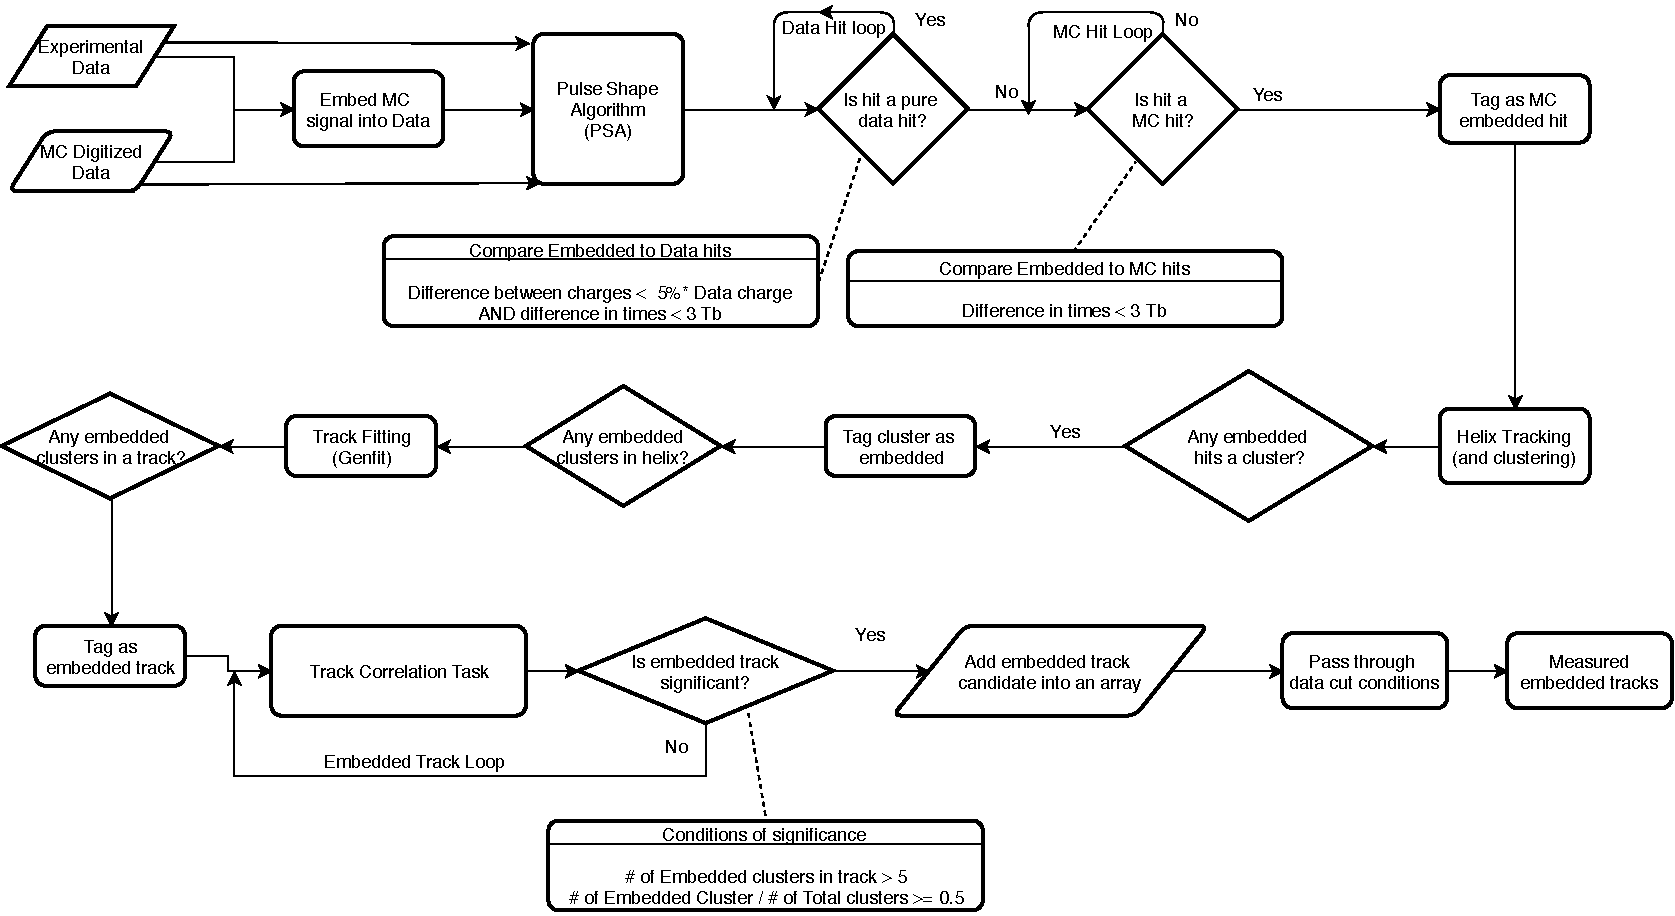
\includegraphics[width=\textwidth]{FlowEmbedding.pdf}
\caption{Flow diagram of the embedding software.}
\label{fig:flow}
\end{figure}

%\end{landscape}
%\pagestyle{plain}

\begin{figure}[!htb]
    \centering
    \begin{subfigure}[t]{0.49\textwidth}
        \centering
        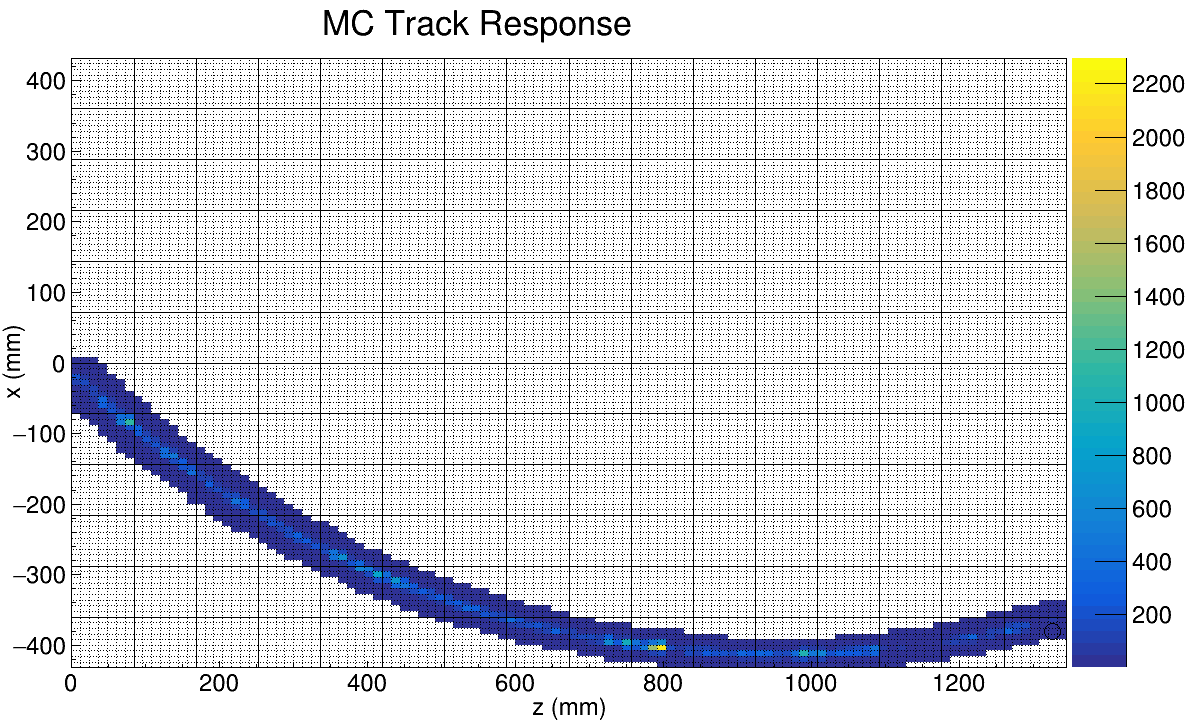
\includegraphics[width=\linewidth]{mcresponse.png}
        \caption{200 MeV/c $\pi^-$ MC digitized track} \label{fig:mcevent}
    \end{subfigure}
    \hfill
    \begin{subfigure}[t]{.49\textwidth}
        \centering
        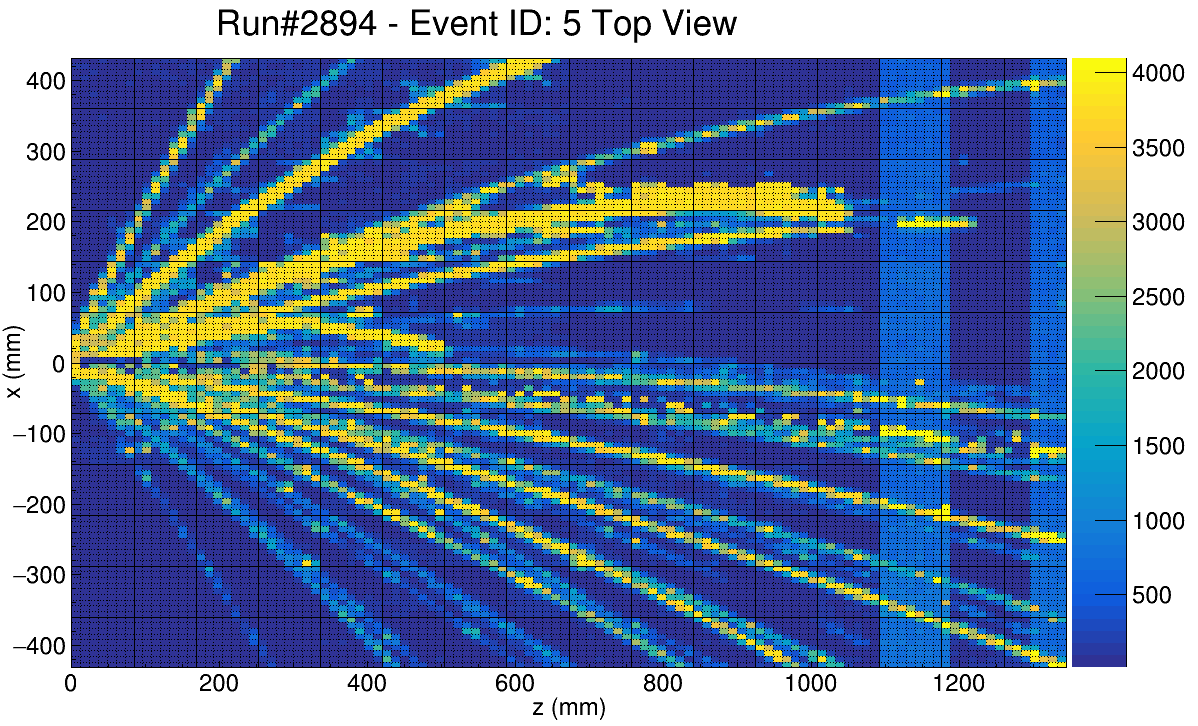
\includegraphics[width=\linewidth]{event5.png} 
        \caption{Experimental data event.} \label{fig:dataevent}
    \end{subfigure}
    \caption{}
\label{fig:mcDataEmbedtrack}
\end{figure}



\begin{figure}[!htb]
    \centering
    \begin{subfigure}[t]{0.49\textwidth}
        \centering
        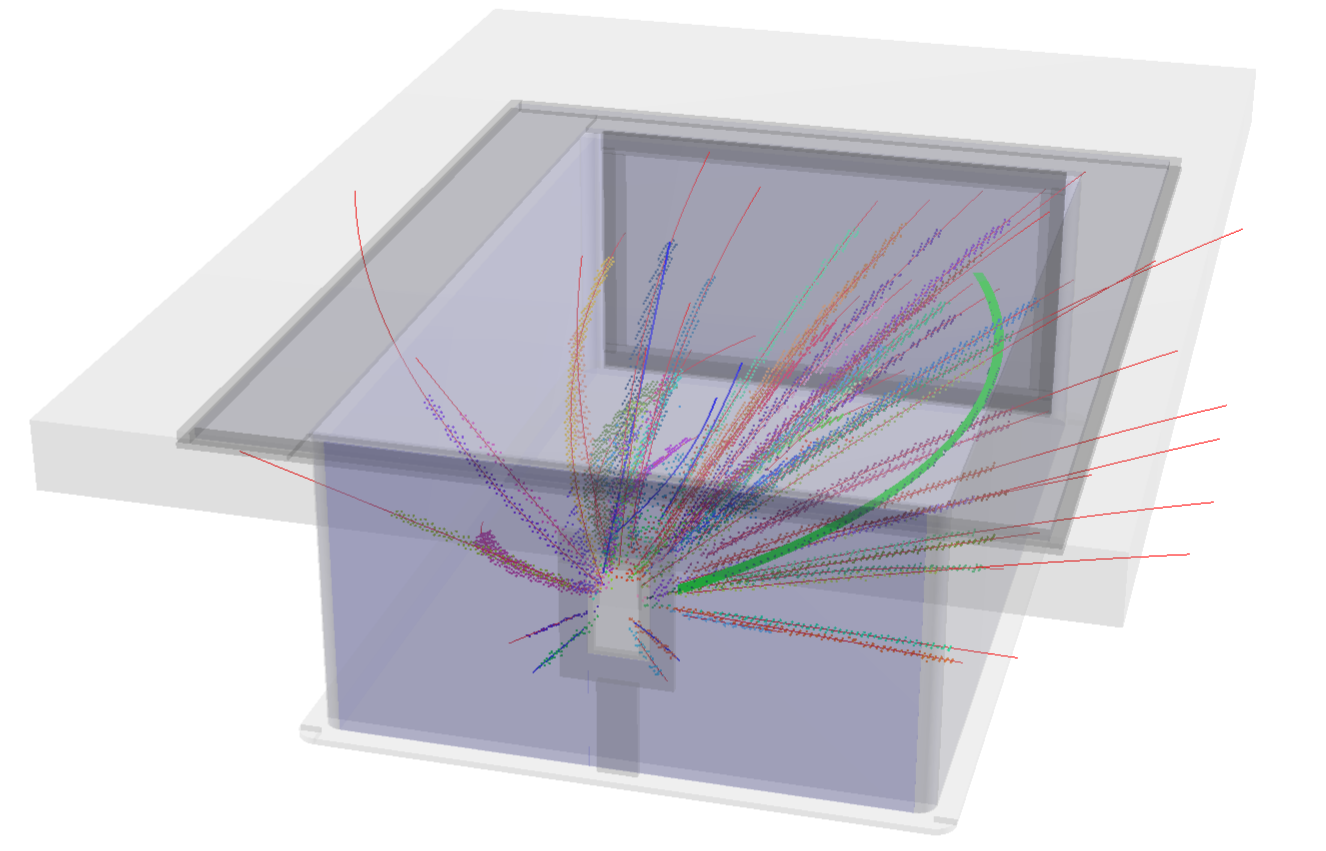
\includegraphics[width=\linewidth]{perspective_embed}
        \caption{Perspective view.} \label{fig:persEmbed}
    \end{subfigure}
    \hfill
    \begin{subfigure}[t]{.3\textwidth}
        \centering
        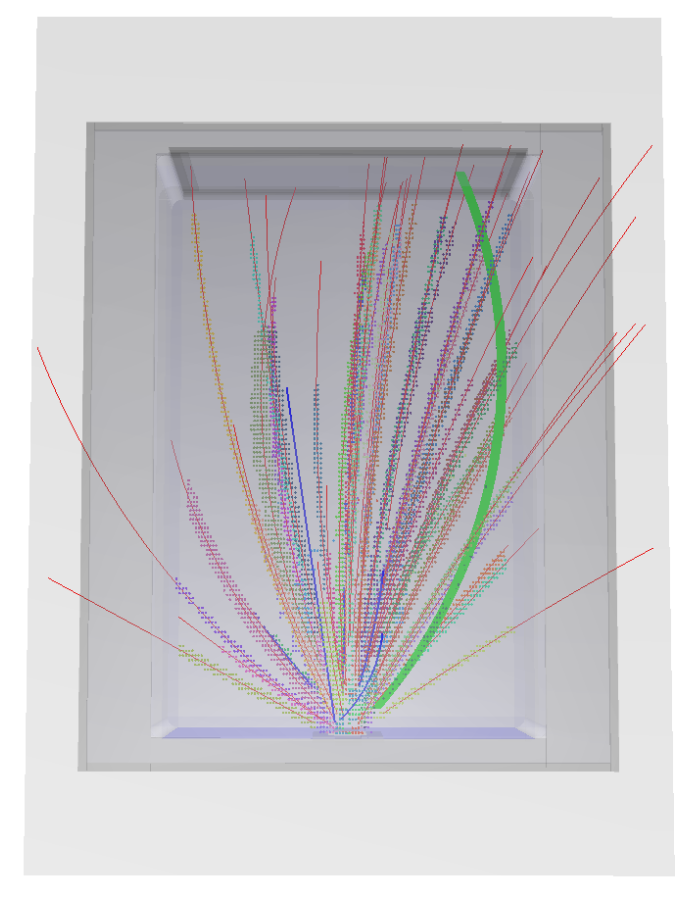
\includegraphics[width=\linewidth]{top_embed} 
        \caption{Top down view.} \label{fig:topEmbed}
    \end{subfigure}
     \hfill
    \begin{subfigure}[t]{\textwidth}
        \centering
        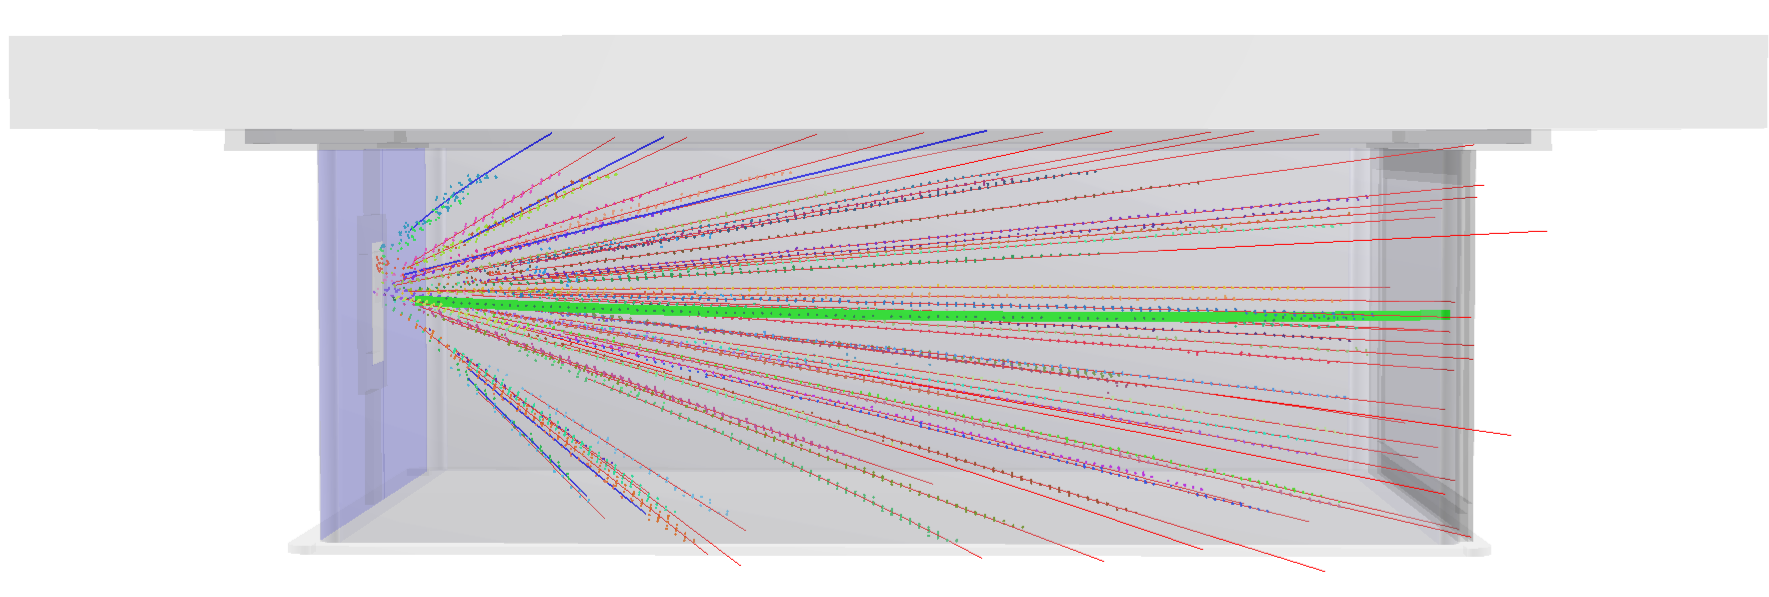
\includegraphics[width=\linewidth]{side_embed} 
        \caption{Side view.} \label{fig:sideEmbed}
    \end{subfigure}
    \caption{A 200 MeV/c $\pi^-$ embedded into a nuclear collision type event. The embedded track identified by the software is highlighted by the solid green line. }

\label{fig:embedtrack}
\end{figure}


The detailed flow diagram of the software implementation of embedding algorithm is shown in Fig.~\ref{fig:flow}. Starting from Geant4 and passing through the 3 MC tasks described above, the output response of the MC track in the TPC is created. From here we directly embed the MC signals into data by adding the MC signals into the data time bucket spectrum, pad-by-pad. As described in Sec.~\ref{sec:simSat}, prior to embedding the MC signals, all pads which are saturated in the experimental data are identified and flagged. The MC signals are forbidden to be embedded after the MC saturation time bucket value. Figure~\ref{fig:mcevent} shows the response of a 200 MeV/c $\pi^-$ track in the TPC; we have embed this track into the data event, Fig.~\ref{fig:dataevent}, just as an example. We will refer to experimental data with embedded MC signals as ``embedded data" for short, the MC generated response as ``MC data", and data only containing only the experimental signals as ``experimental data". The three set of data are each independently analyzed by the PSA algorithm described in Section~\ref{sec:psa},  which finds all the hits associated with each data set. From this the three independent hit data sets are temporarily stored. 

Here within the PSA algorithm, is the first and most important part of the embedding software. The PSA task has the job to identify which hits in the embedded data set originate from the MC hits set and which are from the experimental data. Once the MC hits are identified, these embedded hits can be tagged and tracked through the entire software. 

First, the hits in the embedded set are matched against the experimental data, identifying which of the embedded hits originate from the experimental hit set. For two hits to match, they must satisfy two criteria, $\left|(Q_{\mathrm{Data}} - Q_{\mathrm{Embed} })/Q_{\mathrm{Data}}\right| < .05$ and $\left|t_{\mathrm{Embed} } - t_{\mathrm{Data} }\right| < 3$ where $Q$ and $t$ represent the charge and time of the hit respectively. Hits that satisfy these criteria are then removed from the embedded data set.

The surviving hits are then compared with the MC hit data set, where the criteria for a matching MC hit is, $\left|t_{\mathrm{Embed} } - t_{\mathrm{MC} }\right| < 3$.  There is no requirement for a matching criteria for the charge values which would artificially bias the charge values selected depending on our cut; which is critical for minimum ionizing particles such as pions.  This can only be accomplished by first removing almost all of the experimental hits as was done in the first step. Each embedded hit that passes this step of criteria is tagged as a originating from a MC hit. From here, the embedded data is treated as if it were real data passing through the same software analysis. 

 If a helix track has one hit that is embedded it will also be tagged as embedded. When the hits in a helix track are clustered, if a cluster contains one embedded hit it is itself tagged as an embedded cluster. Furthermore, if a track that is reconstructed contains any embedded clusters, it is tagged as an embedded track. The goal of this na\"ive tagging approach is to preserve all the information of where the embedded hits, clusters, and tracks have gone, preserving as much information until the end without introducing a bias.
 
  It is the job of the embedded correlation task to identify which of the final embedded tracks are candidates for the original input track. For example, several things may happen along the process of embedding that may disqualify a track as a candidate in this na\"ive tagging. A track could break up, lose or share its charge with and adjacent track; it may be not be identified at all for a variety of other reasons. For the embedded track to be a candidate of the input MC track, it must satisfy two conditions, $N_{sat} > 5$ and $N_{\mathrm{sat}}/N_{\mathrm{Total}} \geq .5$, where $N_{\mathrm{sat}}$ is the number of saturated clusters in a track, and $N_{\mathrm{Total}}$ is the number of total clusters. The first criteria is a simple minimum cut where to ensure the minimum condition of a embedded track is met at least having 5 clusters. The second criteria is the strongest cut, ensuring the track has at least half of its clusters coming from embedded MC signals. The set of tracks which satisfy both conditions are saved into an array of candidate tracks. In this way the user can decide how to sort these tracks for studying either efficiency or track splitting. 

If the embedded track is split into multiple tracks, the user must select what they believe to be the track which most represents the original track, for the purposes of calculating efficiency. Typically only one of the tracks in the set will satisfy one of the reasonable quality cut conditions in an analysis. For example the most reasonable assumption is the track originating from the vertex is the most correct in this case, where as the split fraction of the track wont originate from the vertex but instead have a large distance to vertex value. In this thesis, the track with the minimum distance to vertex is identified as the track in which the efficiency analysis will be performed.



\subsection{Simulating Saturation}
\label{sec:simSat}

In general all amplifiers have a finite range of output values set by a positive and negative rail (typically -12V and +12V). If the input charge into a charge sensitive pre-amplifier causes the output voltage to reach the max (or min) output voltage, the electronics is considered saturated and the response may be non-linear. The picture is complicated by the fact that there is usually an RC feedback loop which dissipates the input charge. The time a pre-amplifier returns to linear behavior depends on the input charge and how quickly it can be dissipated \cite{akiGET}. The pad is otherwise considered dead and no further charge can be measured until the channel can recover. There are several types of saturation that must be simulated or accounted for to correctly model the TPC response. They all are varying degrees of the same effect which manifest in different ways in the detector. 
 
Due to the long, high energy tail in  the energy loss distribution of a particle traversing matter, it is common to see pads along the track which have collected large energy loss values saturating the electronics of a couple of pads. This occurs for all tracks, even for minimum ionizing tracks. Saturation in this case is infrequent and not an issue as there are many other clusters are not saturated. As the charge of the particle gets higher, or the momentum gets lower, the  energy loss value also becomes higher, and a significant fraction of pads in a track may be saturated. In Section~\ref{sec:desat}, we outlined an algorithm to correct for the saturation for a  particular track, but this saturation also affects surrounding tracks. In order to make an accurate MC simulation, we must understand how saturation affects surrounding tracks. 

Pads that saturate have no signal or ''dead" for a given amount of time  after the saturating signal, which depends on the amount of input charge. For charges that are at or above the level of the dynamic range, the pad will certainly be dead for the remaining time of the measurement.  Signals from tracks passing directly underneath this pad, with signals that would arrive later in time,  will therefore not be observed. In a sense the saturated pad is ``shadowing" any future tracks. As the track multiplicity of an event increases, the probability of track shadowing increases. This will change event by event and is very difficult to simulate except through a MC track embedding approach, which will be discussed in Section~\ref{sec:embedding}. 

\begin{figure}[!htb]
\centering
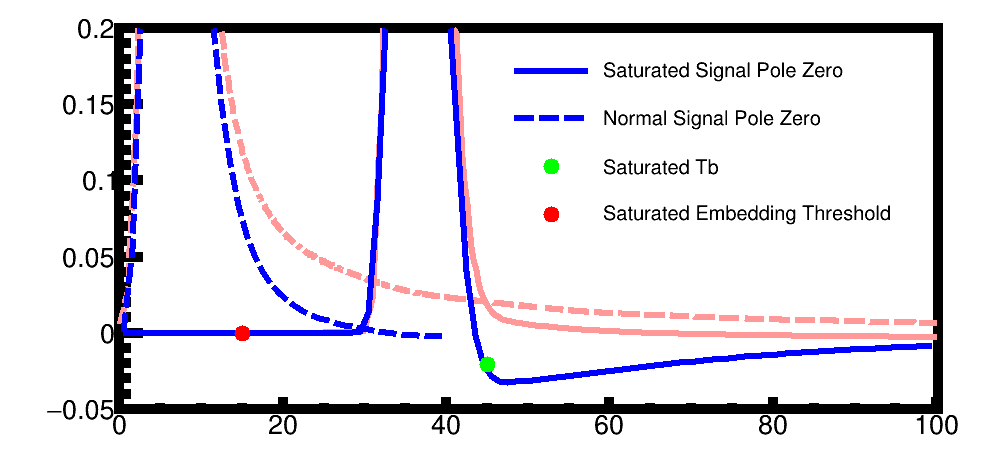
\includegraphics[width=\linewidth]{satpulsepz.png} 
\caption{Example of the pole zero correction when applied to the normal pulse and saturated pulse.} 
\label{fig:pulseSatTag}
\end{figure}


When the input signal is very large, the electronics can be dead for up to \SI{35}{\milli\second} \cite{akiGET}. The beam rate in the experiment was about \SI{10}{\kilo\hertz}, which corresponds to an average of \SI{100}{\micro\second} between subsequent beams. In this case, channels can be effectively dead for several events before recovering. There is a large amount of high energy electrons, commonly referred to as ``delta rays",  which are produced from the beam passing through the gas, due to the high atomic charge of the beam. Horizontally almost all of the electrons cannot travel very far, even for very high energy electrons, due to the vertical magnetic field causing them to curl in tight circles. Figure~\ref{fig:deltaE} shows the horizontal and vertical extent of the delta rays in a top down and side views of the TPC. While many electrons can stop in the gas, some electrons have a high enough kinetic energy in the vertical direction where they can penetrate the gating grid without being blocked. Then they either terminate on the anode wire or possibly deposit their charge directly in the pad. In either case, the charge induced on the pad is large enough to kill the pad for a time long enough to last until at least the next event. This manifests as random dead pads in the experiment, that follow the beam path.  


\begin{figure}[!htb]
    \centering
    \begin{subfigure}[t]{0.49\textwidth}
        \centering
        \includegraphics[width=\linewidth]{deltaE_topview_neg} 
        \caption{Top view} \label{fig:deltaE_topview}
    \end{subfigure}
    \hfill
    \begin{subfigure}[t]{0.49\textwidth}
        \centering
        \includegraphics[width=\linewidth]{deltaE_sideview_neg} 
        \caption{Side view} \label{fig:deltaE_sideview}
    \end{subfigure}
    \caption{Geant4 simulation of ${}^{108}$Sn beam at 270 MeV/A in P10 gas. Notice the extent of the delta electrons in the vertical direction as compared to the horizontal extent. }
\label{fig:deltaE}
\end{figure}


\begin{figure}[!htb]
\includegraphics[width=\textwidth]{padplane_sat.png}
\caption{Results of the algorithm to tag saturated pads, where the black dot denotes a pad was saturated. The charge values plotted is the maximum charge in the pad plane for the entire event.}
\label{fig:satTag}
\end{figure}

The simulation saturation effects is handled naturally by embedding MC tracks into real data; once the time bucket of the saturating signal has been identified, simply no further signals are embedded since the pad is assumed to be dead. In the case a pad is dead for the whole event, the time of saturation is set to the first time bucket and no signal is embedded for any time bucket. We only need to identify where the time of saturation occurs. The characteristic signature of a saturated signal is the fast fall time of a pulse, which quickly reaches zero, as opposed to the long tail of normal pulses as seen in Fig.~\ref{fig:pulseshape}. The long exponential tail can be effectively removed by a simple software technique which is similar to the electronics concept of ``pole-zero compensation". If the raw ADC value at a particular time, $i$, is represented as $f_i$, the corrected pulse which differentiates out the exponential tail, $f_i^{'}$ can be expressed as, 

\begin{equation}
f_i^{'} = \frac{-b_1\cdot f_{i-1}^{'} + a_o\cdot f_i + a_1 \cdot f_{i-1}}{b_o}
\label{eq:satpolez}
\end{equation}

where $a_o$ = .9723, $a_1$=-.9453, $b_o$=.9545, and $b_1$=-.9203. These coefficients were tuned to remove the long tail of the standard non-saturating pulse, without producing any negative undershoots. If the same procedure is applied to the saturated pulse, the correction produces a negative undershoot, since there was no long exponential tail to begin with. Figure~\ref{fig:pulseshape} shows the pulses as the red curves, and after the pole-zero correction as the blue curves for both the normal and saturated pulses. 

By applying this technique to the real data we can identify whether a pad has a saturating pulse in it by looking for this negative undershoot. A negative peak is identified as a saturated signal if it exceeds the threshold of less than -20$\cdot G$ ADC for more than 8 time buckets and the max ADC value is > $G\cdot$500; $G$ is the gain calibration coming from low gain sections discussed in Section~\ref{sec:anodeCalib}. The max ADC condition eliminates false positives which come from  dead pads where the gating grid subtraction is still applied, introducing large false negative peaks, but have no positive signals. After meeting these two conditions, the pad is flagged as saturated and the time bucket position of saturation is set to $t_{peak} - 5$, where $t_{peak}$ is the time bucket position of the negative peak. This is because the falling edge since the falling edge is around 5 time buckets after the beginning of the saturation. A separate time is also stored called the MC time bucket position, which sets the point in time in which a signal cannot be embedded any further. This time is set to $t_{peak} - 30$ to ensure that the MC embedded signals do not overlap the real saturating data signal, which would be impossible. These two positions are also shown in Fig.~\ref{fig:pulseSatTag}.

There is another way a pad can saturate which occurs when all the pulse heights within the time bucket spectrum add to more than the max ADC threshold of 3500 ADC. This arises because the fall time of the pre-amplifier circuit is much longer than the time bucket measurement window, and pulses are allowed to pile up in the pre-amplifier. In this case no single pulse will reach over the max ADC value yet the last pulse will have a pulse shape that is missing the long characteristic tail, but otherwise looks like a normal pulse. These pulses are also identified by the algorithm described above, since this type of saturated pulse is still no long tail.  When embedding signals into pads, we do not consider the previous amount of total charge in the pad. We assume this type of saturation is a higher order correction, where and the current algorithm approximates most of the saturation effects.  Figure~\ref{fig:satTag} shows all of the pads in an event which are tagged by the algorithm as saturated, denoted by the black dots. The max ADC values in a pad are shown in the z-axis color scale, to give a sense of the success of the algorithm. It may appear that the ADC values of some pads appear to be lower than 3500 ADC, but upon further inspection they all satisfy the mode of saturation where the total sum of heights is greater than the max ADC value as described earlier. 

Dead pads are identified earlier in the software when reading in the raw data (STCore class). A dead pad is simply a pad which only contains electronic noise and no signals. A dead pad is identified by having a total ADC r.m.s. value  of less than 50 ADC and a max ADC < 50 over the full time bucket spectrum. Here the dead pad is also tagged as saturated and the time bucket position of saturation is set to the first time bucket, or time zero. 

%NEED TO ADDRESS WHY THE MAX ADC THRESHOLD IS 3500
%maybe simple pream fig
%maybe example from aki paper about times
%maybe 

%Add figure showing saturated time bucket spectra with location of saturation identified and with pulse shape from embedding I would like to add and how it blocks it.
%Add Figure with 2D pad plane response with and without saturation flag

\subsection{MC and Data Comparison}

Here we compare several important observables to ensure the MC is simulating the data sufficiently. These observables will be relevant later in the discussion of quality cuts and efficiency analysis discussed in Section~\ref{sec:efficiency}. The most important observable is the total number of clusters. The number of clusters in a track depends on the geometry of the TPC, the spherical angles of the track, and the clustering algorithm. MC tracks were embedded into data for several particle types. The input angular and momentum distribution was uniform where the final distributions were weighted such that the angular and momentum distribution matched that of the data for a fair comparison. Figure~\ref{fig:clustcomp} shows the normalized cluster distributions for the MC and data for several particle types. There is no data below 20 clusters because this is the minimum cut to ensure quality PID lines in the data. The normalization is changed for each particle type to display them on the same scale. Very good agreement is seen between the MC and data over a wide range of particle species. 

\begin{figure}[!hbt]
\includegraphics[width=\linewidth]{numcluster.png}
\caption{Comparing the distribution of the number of clusters in MC embedded tracks to experimental data.}
\label{fig:clustcomp}
\end{figure}

The second most important observable is the distance-of-closest-approach (dOCA) to the vertex. Figure~\ref{fig:pocacomp} shows the dOCA distributions for the MC embedded tracks and the data, for the same range of particle species. The distributions were again normalized to different values to display on the same scale. Here the only other cut was the  track number of clusters cut > 20, which cleaned up the background spectrum. It is also worth mentioning the data plotted is also after the space charge correction. Before the space charge correction the distributions would be much wider. Since we correct for the space charge in the data we compare here to the embedded MC without any space charge effects, making a fair comparison. 

\begin{figure}[!hbt]
\includegraphics[width=\linewidth]{poca.png}
\caption{Comparison of the dOCA distribution of MC embedded tracks to data.}
\label{fig:pocacomp}
\end{figure}


We can also see good agreement between the MC PRF for $\pi^-$ in Figure~\ref{fig:prfpimMC}, and the data PRF, Fig.~\ref{fig:prfpimData}, where the black line is the PRF fit to the experimental data. It is sufficient to use such a simple universal PRF function as we can describe all the crossing angle effects discussed in \ref{sec:prf}. Therefore these effects must arise from geometric effects related to the track angle, the amount of charge distributed over an anode wire, and the superposition of the PRF from neighboring anode wires which contribute to the appearance of a changing PRF.

\begin{figure}[!htb]
         \centering
         \includegraphics[width=\textwidth]{PRFs_MC_wcut.png}
         \caption{PRF response of the MC $\pi^-$ tracks.}
         \label{fig:prfpimMC}
\end{figure}


%Add Figure of Pad response function for pion,proton.... for MC vs Data vs angles...
%Add Figure of Number of clusters of MC vs Data
%Add Figure of dEdx MC vs Data
%Add Figure of Momentum resolution MC vs Data
%Add Figure of track residuals? MC vs data?


%\section{Aligning TPC}

%explain the different shifts in the TPC
%BDC shift
%Hit offshet shift




\section{Efficiency Corrections}
\label{sec:efficiency}

Since the \spirit TPC is a fixed target experiment it's angular coverage is certainly not 4$\pi$. Because the target is several cm away from the widow of the field cage the geometric acceptance is not even 2$\pi$. The rectangular design complicates the calculation of the geometric acceptance, or the efficiency. Because of this there are regions of the TPC where it is impossible to reconstruct a track due to the geometric in these regions the efficiency is exactly 0. In the regions of non-zero efficiency, the efficiency is a function of at least three main parameters that define the phase space of a track, momentum $p$ and the two spherical lab angles $\theta_{Lab}$ and $\phi_{Lab}$. 

The track efficiency $\epsilon$ is calculated bin-by-bin and is simply written as, 
\begin{equation}
\epsilon = \frac{n_{reco}}{N},
\end{equation}

where $n_{reco}$ is the number of embedded tracks which are successfully reconstructed, and $N$ is the total number of input embedded tracks for that given bin. A track is defined to be successfully reconstructed if it exists in the correlation task described in \ref{sec:embedding}, and therefore meets the minimum criteria for an embedded track, and if it passes the various quality cuts performed on the experimental data set; this could be angular cuts, PID cuts, etc. The TPC response will introduce a finite resolution in both the angles and the momentum. Because of the final measured track could have migrated out of the input bin into another bin. The bin-by-bin correction method is only valid if this effect is small as compared with the size of the bin. If not a more complicated un-folding procedure is needed. The efficiency is defined as the number of all tracks that were reconstructed and passed the cuts successfully, even if some had migrated to other bins, the efficiency value is assumed to represent the center of the input MC bin.  
%TALK ABOUT BIN SIZES HEREE????? 

 Single MC tracks are embedded into a set of \num{e4} on target events and the measured output tracks are correlated to the input track from the embedding software. If the track split in the analysis software, and there are several tracks identified by the software as an embedded track, or part of one, we certainly cannot double count the track as the efficiency is  defined strictly as $\epsilon < 0$. In this case, the track with the minimum distance to vertex is taken for the purposes of calculating efficiency. This is because in the case the track splits, it is very rare for the later segments of the track to have a distance-to-vertex which originates from the target region. It's reasonable to assume the track with the minimum distance to vertex is the track that best represents the ``real" track. The embedded MC tracks are generated as a uniform distribution in $\theta$,$\phi$, and $p$, to ensure each bin has as similar number of input tracks $N$, giving approximately the same statistical error. Here the efficiency distribution is independent of the initial input distribution since we were careful to not assign tracks that migrated out of the input bin, into another bin, which would make the efficiency biased by the input distribution. 
 
\begin{figure}[!htb]
    \centering
    \begin{subfigure}[t]{0.49\textwidth}
        \centering
        \includegraphics[width=\linewidth]{pim_200_pol.png}
        \caption{Polar efficiency plot where $\theta$ is represented by the radius of the circle and $\phi$ is measured as the polar angle made between the y and x axis; this view is  best understood as looking at the TPC from the downstream point of view.} \label{fig:pim_pol_eff_ex}
    \end{subfigure}
    \hfill
    \begin{subfigure}[t]{.49\textwidth}
        \centering
        \includegraphics[width=\linewidth]{pim_200_efficiency.png} 
        \caption{Cartesian representation of the same efficiency plot  as in the polar plot.} \label{fig:pim_flat_eff_ex}
    \end{subfigure}
  
\caption{Efficiency calculations for $\pi^-$ particle traveling at \SI{200}{\mega\eVperc}.}
\label{fig:pim_eff_ex}
\end{figure}
 
 
 
Figure~\ref{fig:pim_eff_ex} shows the efficiency calculated for $\pi^-$ tracks traveling with momentum \SI{200}{\mega\eVperc} as a function of the two laboratory angles. It is easiest to visualize the efficiency distribution first in a polar representation which is most like viewing the actual TPC progressing to a visualization that is easier to see the values. Figure~\ref{fig:pim_pol_eff_ex} shows the efficiency values plotted in a polar representation where $\theta_{Lab}$ is represented as the radial dimension and $\phi$ is represented as the polar angle. This way is best understood as if one looked at the TPC from the downstream point of view. Of course the vertical direction of the TPC,$\phi$=\ang{90}, is limited in vertical space, therefore tracks are not reconstructed well. The same is the case in downward going tracks, the region centered around $\phi$=\ang{270}. The best regions are seen by the high efficiency values which are left and right in the TPC where the rectangular TPC has the highest acceptance. Though this view is the most intuitive to think about in a physical geometry sense, the values of the efficiency in each bin are difficult to see. Figure~\ref{fig:pim_flat_eff_ex} shows the same efficiency plot but plotted in a more standard two dimensional plot. Here we can see even better the acceptance of downward going tracks , $\phi$=\ang{270}, is greater than the dip in upward going tracks, $\phi$=\ang{90}, due to the field cage being centered in the magnet and not in the TPC. 

The area enclosed by the red lines represent the region of the highest efficiency over the full region in $\theta_{Lab}$.  Since we take cuts similar to these in the real data, we assume the efficiency is independent of $\phi$ over these small regions. The efficiency then can be represented as just a function of the two remaining variables. Figure~\ref{fig:132_eff} shows the efficiency of $\pi^-$ and $\pi^+$ particles in the $\tin{132}{124}$ system and Fig.~\ref{fig:108_eff} for the $\tin{108}{112}$ system as a function of $\theta_{Lab}$ and momentum $p_{Lab}$. 



\begin{figure}[!htb]
    \centering
    \begin{subfigure}[t]{0.49\textwidth}
        \centering
        \includegraphics[width=\linewidth]{pim_132_efficiency.png}
        \caption{$\pi^-$ efficiency for $\tin{132}{124}$} \label{fig:pim_132_eff}
    \end{subfigure}
    \hfill
    \begin{subfigure}[t]{.49\textwidth}
        \centering
        \includegraphics[width=\linewidth]{pip_132_efficiency.png} 
        \caption{$\pi^+$ efficiency for $\tin{132}{124}$} \label{fig:pip_132_eff}
    \end{subfigure}
  
    \caption{ }
\label{fig:132_eff}
\end{figure}



\begin{figure}[!htb]
    \centering
    \begin{subfigure}[t]{0.49\textwidth}
        \centering
        \includegraphics[width=\linewidth]{pim_132_efficiency.png}
        \caption{$\pi^-$ efficiency for $\tin{108}{112}$} \label{fig:pim_108_eff}
    \end{subfigure}
    \hfill
    \begin{subfigure}[t]{.49\textwidth}
        \centering
        \includegraphics[width=\linewidth]{pip_108_efficiency.png} 
        \caption{$\pi^+$ efficiency for $\tin{108}{112}$} \label{fig:pip_108_eff}
    \end{subfigure}
  
    \caption{ }
\label{fig:108_eff}
\end{figure}


\section{PID Analysis}
\label{sec:pid}
%PID lines over all picture


%PID of pion cut
%background estimation

The energy loss curve in Eq.~\ref{eq:bb} can be described as a 5-parameter general function as, 

\begin{equation}
\frac{dE}{dx} = \frac{p_0}{\beta^{p_3}}(p_1 - \beta^{p_3} + \ln(p_2 + {\beta\gamma}^{-p_4})),
\label{eq:5par_bb}
\end{equation}

where the parameters $p_0-p_4$ are free parameters, $\beta= p/\sqrt{p^2 + m^2c^4}$, where $m$ is the mass of the particle and $p$ is the momentum. The PID lines vary slightly as a function of the emission angle of each track. The PID was subdivided into 6 pitch angles, $\theta_P = \arctan(p_y/p_z)$, and 6 yaw angles, $\theta_Y = \arctan(p_x/p_z)$, ranging from \ang{-90} to \ang{90} for both. The pion spectra of each yaw-pitch bin was fit with Eq.~\ref{eq:5par_bb} to get the PID line which best describes the data. The distribution around this mean value is not a Gaussian distribution. The variable $z$ has been used before to transform the energy loss of a particular track $dE/dx$ into a more Guassian variable, defined as

\begin{equation}
z_i = \ln\Big(\frac{\langle dE/dx\rangle}{\langle dE/dx\rangle_i}\Big),
\end{equation}

where $\langle dE/dx\rangle_i$ is the mean energy loss curve fit from Eq.~\ref{eq:5par_bb} for a given particle type $i$. The $z_i$ distribution of the particle of interest will be centered around 0 in this new variable. Figure~\ref{fig:pidpion_raw} shows the typical PID lines zoomed in on the pions. Figure~\ref{fig:pidpion} shows the corresponding $z_i$ distribution after all the pitch-yaw bins have been merged. Both charged pions lie on $z_i=0$, where other particle species rapidly diverge. 

\begin{figure}[!htb]
    \centering
    \begin{subfigure}[t]{0.49\textwidth}
        \centering
        \includegraphics[width=\linewidth]{pidPion.png}
        \caption{Output PID pions.} \label{fig:pidpion_raw}
    \end{subfigure}
    \hfill
    \begin{subfigure}[t]{.49\textwidth}
        \centering
        \includegraphics[width=\linewidth]{pidPion_zi.png} 
        \caption{PID plot for $\pi^-$ and $\pi^+$ species in $z_i$. } \label{fig:pipion_zi}
    \end{subfigure}
  
    \caption{$\langle dE/dx\rangle$ versus p/q for $\tin{132}{124}$ system.}
\label{fig:pidpion}
\end{figure}

Now that the pion distribution is flattened, we take bin slices along $p/q$ to determine the particle yield in a certain bin and also estimate the background contribution. The background relevant to  the charged pions comes from the $e^+$ and $e^-$ resulting from the $\pi^0$ Dalitz decay described in Appendix~\ref{appen:dalitz}. Figure~\ref{fig:pimmom_flat} shows the Gaussian fits to the $z_i$ distribution for two different $p/q$ binned cuts around the $\pi^-$ particles, where as Fig.~\ref{fig:pipmom_flat} shows the background $\pi^+$ particles. A Gaussian fit is performed to the pions and to the $e$ spectrum to estimate the background contribution. 


\begin{figure}[!htb]
    \centering
    \begin{subfigure}[t]{0.49\textwidth}
        \centering
        \includegraphics[width=\linewidth]{pim_mom2.png}
        \caption{Bin -54 MeV/c < p/q < -52. } \label{fig:pimmom2}
    \end{subfigure}
    \hfill
    \begin{subfigure}[t]{.49\textwidth}
        \centering
        \includegraphics[width=\linewidth]{pim_mom1.png} 
        \caption{Bin -68 MeV/c < p/q < -66.} \label{fig:pimmom1}
    \end{subfigure}
  
    \caption{$z_i$ projection for binned slices in p/q around the $\pi^-$.}
\label{fig:pimmom_flat}
\end{figure}



\begin{figure}[!htb]
    \centering
    \begin{subfigure}[t]{0.49\textwidth}
        \centering
        \includegraphics[width=\linewidth]{pip_mom1.png}
        \caption{Bin 74 MeV/c < p/q < 76. } \label{fig:pipmom1}
    \end{subfigure}
    \hfill
    \begin{subfigure}[t]{.49\textwidth}
        \centering
        \includegraphics[width=\linewidth]{pip_mom2.png} 
        \caption{Bin 94 MeV/c < p/q < 86.} \label{fig:pipmom2}
    \end{subfigure}
  
    \caption{$z_i$ projection for binned slices in p/q around the $\pi^+$.}
\label{fig:pipmom_flat}
\end{figure}
